\documentclass[a4paper,10pt]{report}

% ============================================
% DOCUMENT METADATA
% ============================================
\newcommand{\reporttitle}{BÁO CÁO LAB 03 LÝ THUYẾT}
\newcommand{\coursename}{Thị giác máy tính}
\newcommand{\coursecode}{CSC16004}
\newcommand{\classname}{23TGMT}
\newcommand{\semester}{1}
\newcommand{\academicyear}{2025--2026}
\newcommand{\studentname}{Trương Quốc Cường}
\newcommand{\studentid}{23127333}
\newcommand{\advisorone}{TS. Võ Hoài Việt}
\newcommand{\advisortwo}{ThS. Phạm Minh Hoàng}
\newcommand{\advisorthree}{ThS. Phạm Thanh Tùng}
\newcommand{\reportplace}{Thành phố Hồ Chí Minh}
\newcommand{\reportdate}{ngày 27 tháng 3 năm 2026}
\newcommand{\repourl}{https://github.com/TQC0103/Lab3_LT_TGMT}

% ============================================
% PACKAGES
% ============================================
\usepackage[left=0.75in,right=0.75in,top=1in,bottom=1in]{geometry}
\usepackage{fontspec}
\usepackage{polyglossia}
\usepackage{setspace}
\usepackage{graphicx}
\usepackage{tikz}
\usetikzlibrary{calc}
\usepackage{float}
\usepackage{placeins}
\usepackage{amsmath}
\usepackage{amssymb}
\usepackage{enumitem}
\usepackage{xurl}
\usepackage{microtype}
\usepackage{longtable}
\usepackage{tabularx}
\usepackage{booktabs}
\usepackage[hidelinks]{hyperref}
\usepackage[style=ieee,backend=biber,language=english]{biblatex}

% ============================================
% FONT CONFIGURATION
% ============================================
\setmainfont{Latin Modern Roman}
\setsansfont{Latin Modern Sans}
\setmonofont{Latin Modern Mono}

% ============================================
% LANGUAGE CONFIGURATION
% ============================================
\setmainlanguage{vietnamese}
\setotherlanguage{english}
\DeclareLanguageMapping{vietnamese}{english}

% ============================================
% SPACING AND FORMATTING
% ============================================
\setstretch{1.15}
\setcounter{secnumdepth}{3}
\setcounter{tocdepth}{2}
\emergencystretch=2em

% ============================================
% BIBLIOGRAPHY
% ============================================
\addbibresource{references.bib}
\AtBeginBibliography{\sloppy}

% ============================================
% VIETNAMESE LABELS
% ============================================
\addto\captionsvietnamese{%
  \renewcommand{\contentsname}{Mục lục}%
  \renewcommand{\listfigurename}{Danh sách hình vẽ}%
  \renewcommand{\listtablename}{Danh sách bảng}%
  \renewcommand{\figurename}{Hình}%
  \renewcommand{\tablename}{Bảng}%
  \renewcommand{\chaptername}{Chương}%
}

% ============================================
% LIST CONFIGURATION
% ============================================
\BeforeBeginEnvironment{itemize}{\par}
\setlist[itemize]{leftmargin=*,labelsep=0.5em}
\setlist[itemize,2]{label=\textopenbullet}
\setlist[description]{style=nextline}

% ============================================
% ACRONYM/GLOSSARY MACROS
% ============================================
\newcommand{\abbrtarget}[1]{\hypertarget{abbr:#1}{}}
\newcommand{\abbrlink}[2]{\hyperlink{abbr:#1}{#2}}
\newcommand{\abbrlinkS}[1]{\hyperlink{abbr:#1}{#1}}

% ============================================
% DOCUMENT BEGIN
% ============================================
\begin{document}

\include{cover}

\fontsize{10pt}{12.5pt}\selectfont

% ======================
% Preface
% ======================
\chapter*{Lời nói đầu}
\addcontentsline{toc}{chapter}{Lời nói đầu}

Báo cáo này được thực hiện trong khuôn khổ môn học \coursename{} tại Trường Đại học Khoa học Tự nhiên, ĐHQG-HCM. Nội dung báo cáo tập trung vào các yêu cầu và bài toán của Lab 03, với mục tiêu trình bày rõ ràng quy trình thực hiện, cơ sở lý thuyết liên quan và các nhận xét rút ra từ kết quả thực nghiệm.

Tài liệu được tổ chức theo hướng thuận tiện cho việc mở rộng trong quá trình làm bài: phần mở đầu nêu bối cảnh và mục tiêu, các chương sau trình bày phương pháp, kết quả và đánh giá. Khung báo cáo này cũng được chuẩn bị để dễ dàng chèn thêm hình ảnh, bảng biểu, công thức và tài liệu tham khảo khi nội dung Lab 03 hoàn thiện.

\vspace{1cm}

\begin{flushright}
\textit{Sinh viên thực hiện}\\
\textit{\studentname}
\end{flushright}

\clearpage

% ======================
% General information
% ======================
\chapter*{Thông tin chung}
\addcontentsline{toc}{chapter}{Thông tin chung}

\begin{tabular}{ll}
\textbf{Tên môn học:} & \coursename \\[6pt]
\textbf{Mã môn học:} & \coursecode \\[6pt]
\textbf{Lớp:} & \classname \\[6pt]
\textbf{Học kỳ:} & \semester \\[6pt]
\textbf{Năm học:} & \academicyear \\[12pt]
\textbf{Giảng viên:} & \advisorone \\
                     & \advisortwo \\
                     & \advisorthree \\[12pt]
\textbf{Sinh viên:} & \studentname \\[6pt]
\textbf{MSSV:} & \studentid \\[6pt]
\textbf{GitHub repo:} & \url{\repourl} \\[6pt]
\end{tabular}

\vspace{1cm}

\clearpage
\addcontentsline{toc}{chapter}{Mục lục}
\tableofcontents
\clearpage

% % ======================
% Glossary
% ======================
\chapter*{Bảng thuật ngữ}
\addcontentsline{toc}{chapter}{Bảng thuật ngữ}

\begin{description}
  \item[CV] Computer Vision.
  \item[ML] Machine Learning.
  \item[DL] Deep Learning.
\end{description}

\clearpage

\chapter{Phân lớp chữ số MNIST Handwritten bằng ANN}

\section{Tổng quan}

Từ phần EDA của Lab 02, có ba insight chính được giữ lại cho Lab 03. Thứ nhất, MNIST là bộ dữ liệu khá sạch, kích thước ảnh đồng nhất và độ tương phản giữa nét chữ với nền đủ rõ để một ANN thuần vẫn có thể học trực tiếp từ raw pixel~\cite{mnist_official}. Thứ hai, một số lớp như $4$, $5$, $8$ và $9$ còn chồng lấn về hình thái; khác biệt nằm nhiều ở hướng nét, độ nghiêng và vị trí tương đối của các stroke hơn là ở cường độ sáng đơn thuần. Thứ ba, biến thiên hình học như nghiêng nhẹ, lệch tâm và thay đổi hình dạng nét vẫn còn hiện diện, nên nếu chỉ dùng raw pixel phẳng thì mô hình rất dễ bám vào biểu diễn cụ thể của ảnh train và tạo ra chênh lệch train-test lớn.

Toàn bộ mã nguồn, notebook Colab, artifact và file báo cáo dùng để tạo ra các thực nghiệm trong chương này được tổ chức trong cùng một repository GitHub tại \url{\repourl}. Vì vậy, các kết quả trình bày dưới đây không chỉ là mô tả lý thuyết mà bám trực tiếp trên pipeline thực nghiệm đã được lưu vết trong repo.

Vì vậy, Chương 1 không đi thẳng tới mô hình cuối cùng mà triển khai theo đúng quá trình thử nghiệm thực tế: bắt đầu từ \textit{naive ANN}, quan sát điểm yếu của nó, rồi lần lượt thêm tiền xử lý, đặc trưng hóa, augmentation và thay đổi cách hợp nhất đặc trưng để giải quyết điểm yếu của biến thể trước đó.

\section{Phát biểu bài toán}

Bài toán cần giải quyết là phân lớp ảnh chữ số viết tay thành $10$ lớp tương ứng với các chữ số từ $0$ đến $9$. Đầu vào của mô hình là một ảnh xám kích thước $28 \times 28$, tức mỗi mẫu ban đầu có $784$ pixel. Đầu ra của mô hình là một vector logits có $10$ phần tử; phần tử có giá trị lớn nhất quyết định nhãn dự đoán cuối cùng của ảnh.

Về mặt dữ liệu, MNIST là bộ dữ liệu \textit{single-label classification}, nghĩa là mỗi ảnh chỉ thuộc đúng một lớp duy nhất~\cite{mnist_official}. Trong Lab 03, dữ liệu được dùng đúng theo hai split chính thức của MNIST, không tách thêm validation riêng. Toàn bộ $60{,}000$ mẫu train được dùng để huấn luyện mô hình, còn toàn bộ $10{,}000$ mẫu test chỉ được dùng để đánh giá cuối cùng sau khi train xong. Cách thiết lập này bám sát yêu cầu của bài lab và giúp việc so sánh giữa các cấu hình ANN được giữ thống nhất.

\begin{table}[H]
  \centering
  \caption{Thống kê dữ liệu và cách sử dụng các split của MNIST trong Lab 03}
  \label{tab:mnist-problem-setup}
  \begin{tabular}{lccc}
    \toprule
    \textbf{Split} & \textbf{Số mẫu} & \textbf{Vai trò} & \textbf{Cách dùng trong Lab 03} \\
    \midrule
    Train & 60{,}000 & Huấn luyện & Dùng toàn bộ để train mô hình \\
    Test & 10{,}000 & Đánh giá cuối & Chỉ dùng để báo kết quả cuối cùng \\
    \bottomrule
  \end{tabular}
\end{table}


\section{Mô hình và tham số}
\subsection{Naive ANN}

Naive ANN là baseline đơn giản nhất và cũng là điểm xuất phát hợp lý nhất để kiểm tra xem ANN thuần có thể học được bao nhiêu từ ảnh gốc. Đầu vào của mô hình là ảnh xám $28 \times 28$ sau khi chia cho $255$ để đưa cường độ sáng về khoảng $[0,1]$. Sau bước này, ảnh được trải phẳng thành vector $x \in \mathbb{R}^{784}$; như vậy lớp vào có đúng $784$ neuron vì mỗi neuron tương ứng trực tiếp với một pixel của ảnh gốc. Đầu ra của mô hình là vector logits $z \in \mathbb{R}^{10}$, nên lớp cuối có $10$ neuron để biểu diễn mười lớp chữ số từ $0$ đến $9$.

Kiến trúc cụ thể của baseline là:
\[
784 \rightarrow 1024 \rightarrow 512 \rightarrow 256 \rightarrow 10.
\]
Ba tầng ẩn dùng ReLU, còn tầng cuối giữ logits thô để đưa vào hàm loss. Cách chọn số chiều ẩn ở đây có chủ đích. Tầng đầu tiên tăng từ $784$ lên $1024$ để mở rộng không gian biểu diễn, vì raw pixel ở dạng phẳng còn rất nghèo về ngữ nghĩa; nếu vừa vào mạng đã nén xuống nhỏ hơn $784$ thì mô hình rất dễ làm mất các tương quan cục bộ giữa các stroke. Sau khi đã có một tầng đủ rộng để tái tổ hợp các pixel thô, số chiều được giảm dần về $512$ rồi $256$ nhằm ép mạng học biểu diễn cô đọng hơn trước khi đi tới lớp phân loại.

Việc giảm dần số chiều ở các tầng sau được chọn vì đây là baseline cần một luồng xử lý ổn định và dễ diễn giải: tầng đầu rộng để hấp thụ thông tin thô, các tầng sau hẹp dần để lọc bớt nhiễu và giữ lại đặc trưng cần thiết cho phân lớp. Nếu tiếp tục làm các tầng sau ngày càng rộng hơn nữa, mô hình sẽ có quá nhiều tự do biểu diễn trên bộ đặc trưng vốn đã rất thô, từ đó tăng nguy cơ ghi nhớ train set thay vì học cấu trúc chung. Nói ngắn gọn, baseline này cố ý giữ kiến trúc ``mở rộng một lần rồi nén dần'', thay vì ``càng sâu càng rộng'', để cân bằng giữa năng lực biểu diễn và khả năng tổng quát hóa.

Hàm loss được dùng là \textit{cross-entropy loss}. Đây là lựa chọn tự nhiên cho bài toán \textit{single-label classification} vì mỗi ảnh chỉ thuộc đúng một lớp. Về mặt động lực học, cross-entropy buộc logit của lớp đúng phải tăng lên tương đối so với chín lớp còn lại, thay vì chỉ tối ưu từng lớp độc lập. Điều này phù hợp với bài toán chữ số, nơi mười lớp loại trừ lẫn nhau. Optimizer được dùng là Adam với learning rate $10^{-3}$ và weight decay bằng $0$. Adam được chọn cho baseline vì nó hội tụ nhanh, ít cần tinh chỉnh hơn SGD trong những lượt thử đầu, và giúp nhanh chóng kiểm tra xem ANN thuần trên raw pixel có đang học đúng hướng hay không trước khi thêm các kỹ thuật mạnh hơn như BatchNorm, Dropout hay HOG.

Mô hình này không dùng \textit{deslant}, \textit{recenter}, HOG, BatchNorm, Dropout hay augmentation. Chính vì thiếu toàn bộ các thành phần đó, nó đóng vai trò mốc tối thiểu: nếu baseline đã bộc lộ rõ loại lỗi nào, các biến thể sau sẽ được thiết kế trực tiếp để xử lý loại lỗi đó.


\begin{figure}[H]
  \centering
  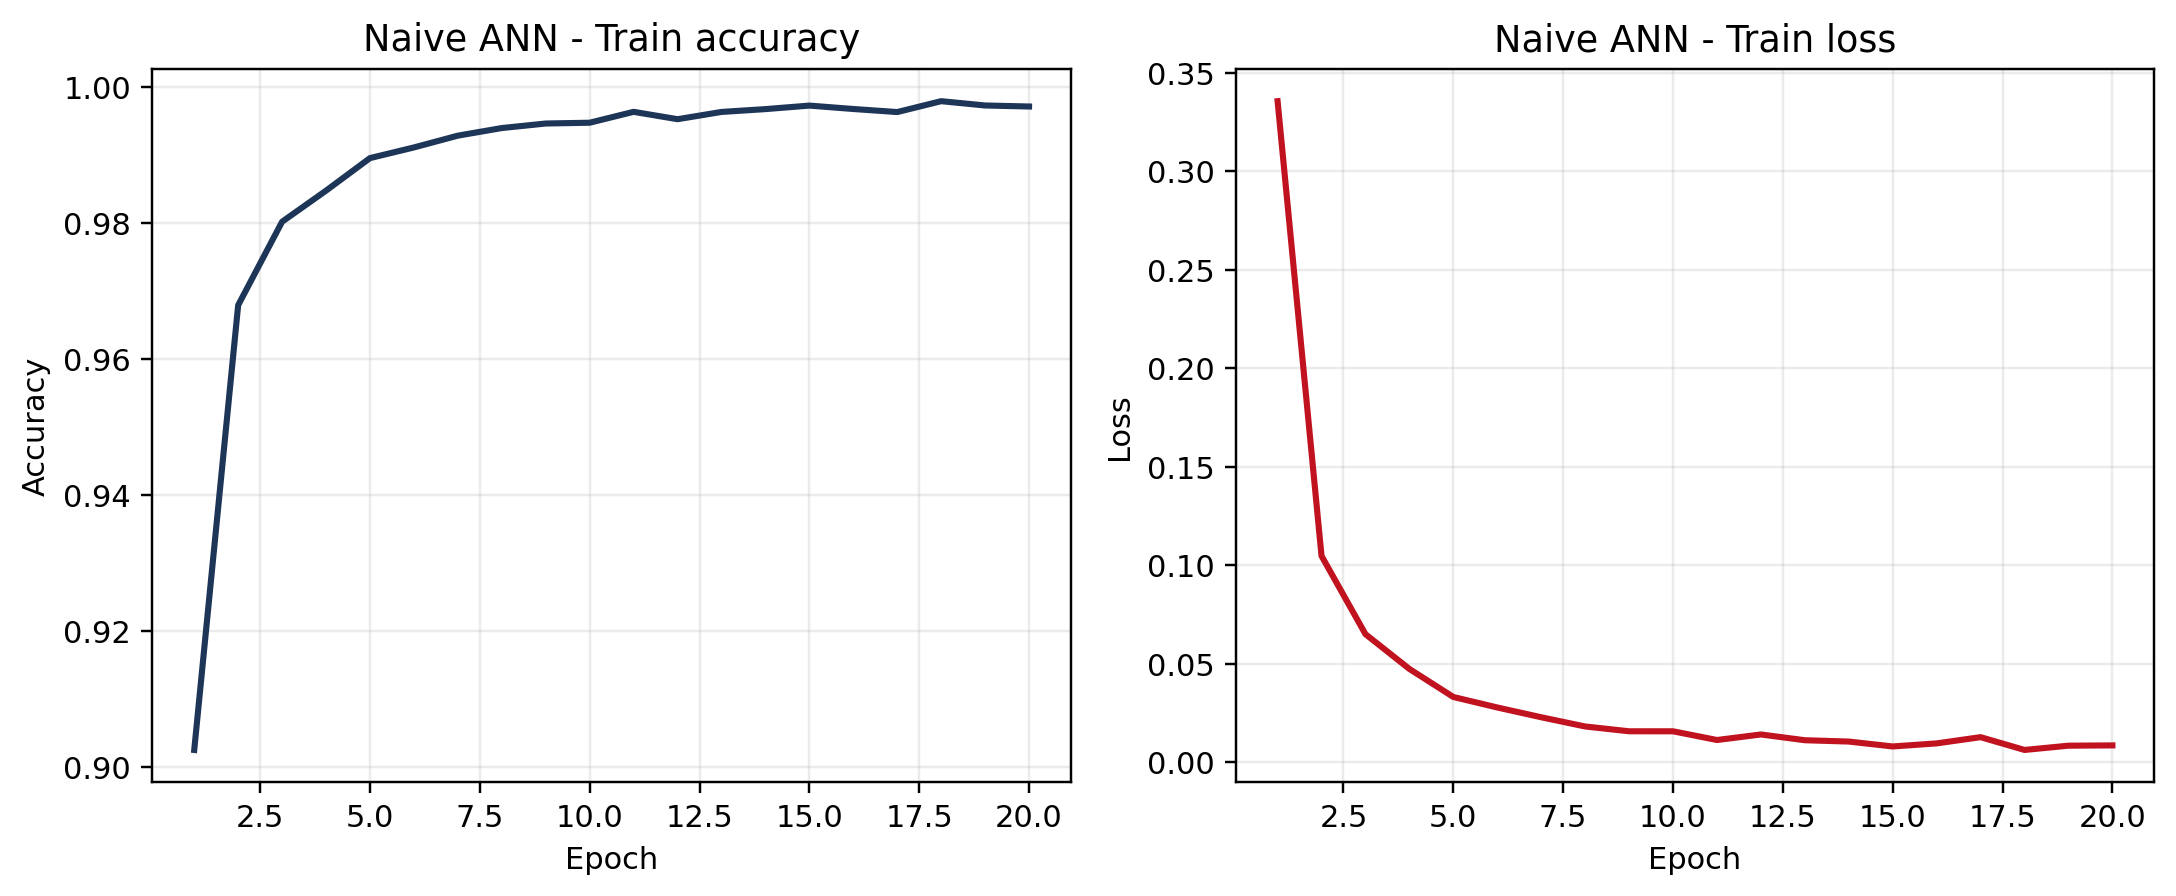
\includegraphics[width=0.92\textwidth]{figures/mnist-models/naive_training_curves.png}
  \caption{Diễn biến train accuracy và train loss của Naive ANN.}
  \label{fig:mnist-naive-training}
\end{figure}

\begin{figure}[H]
  \centering
  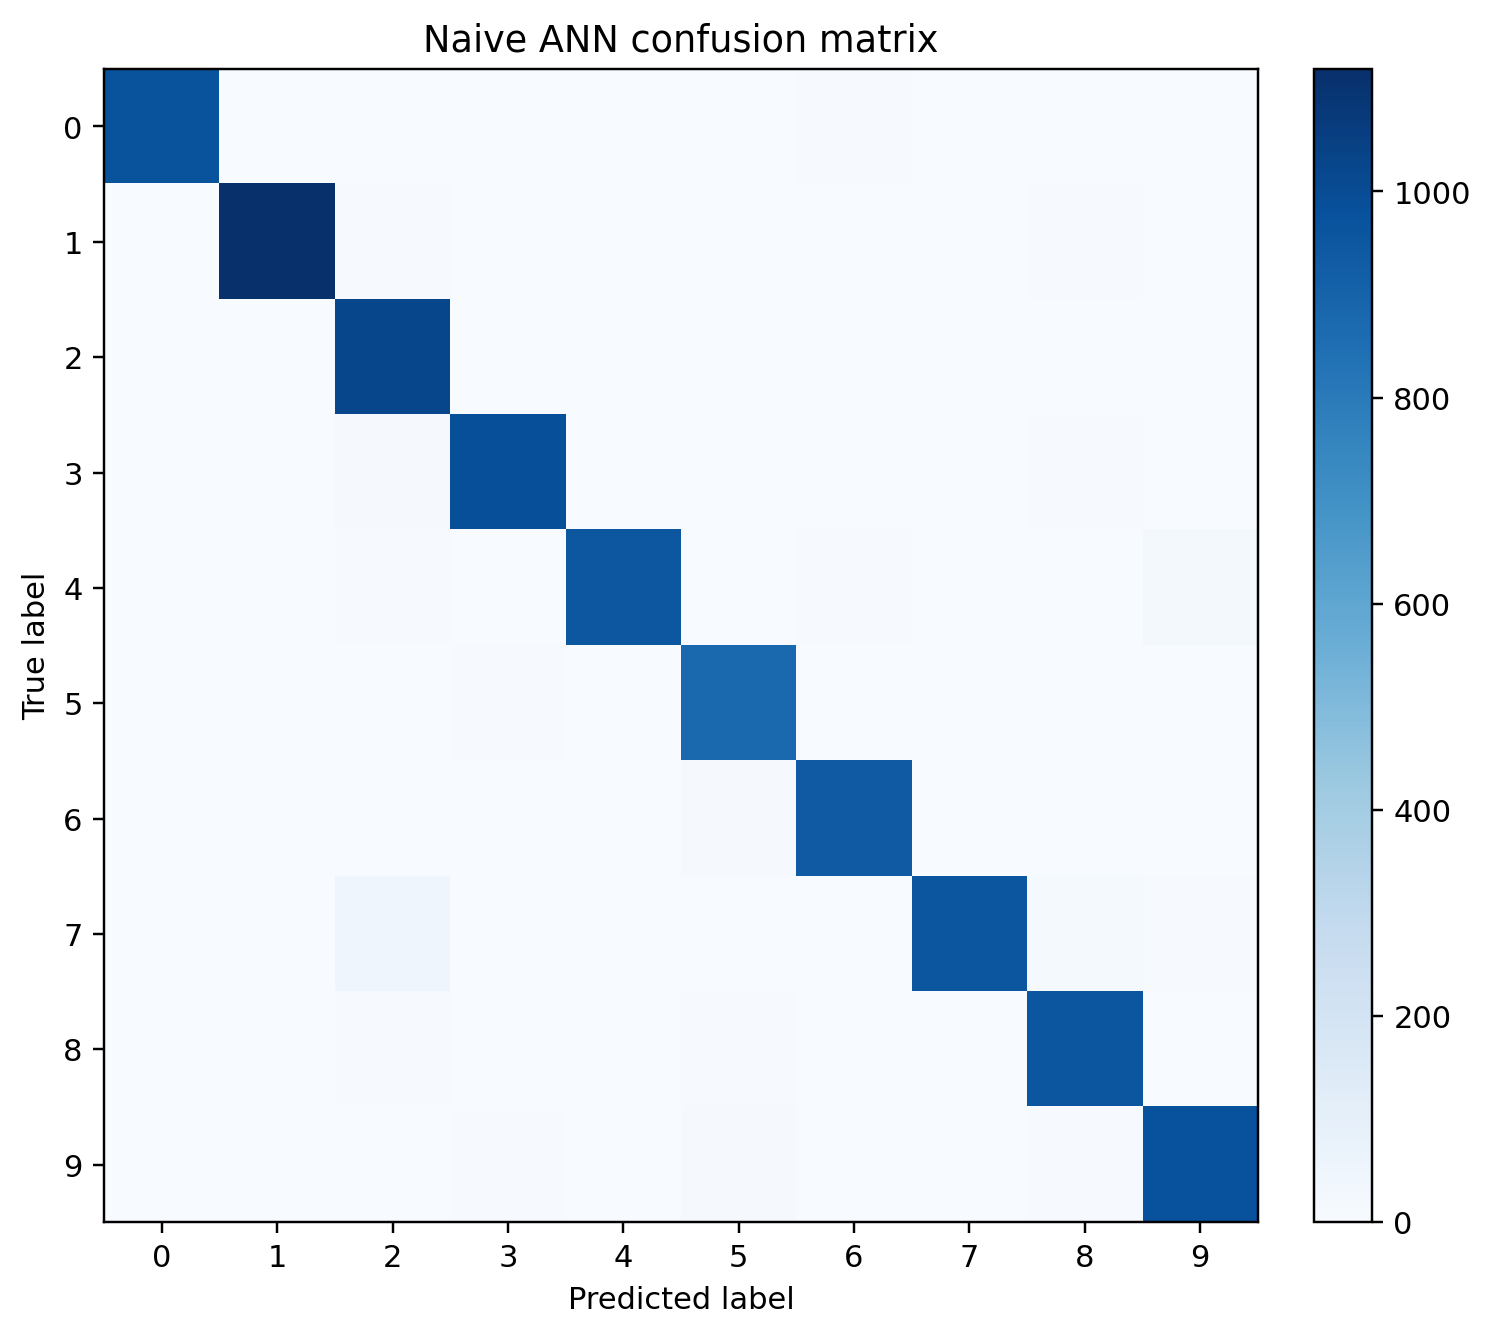
\includegraphics[width=0.72\textwidth]{figures/mnist-models/naive_confusion_matrix.png}
  \caption{Confusion matrix của Naive ANN trên tập test MNIST.}
  \label{fig:mnist-naive-confusion}
\end{figure}

\begin{figure}[H]
  \centering
  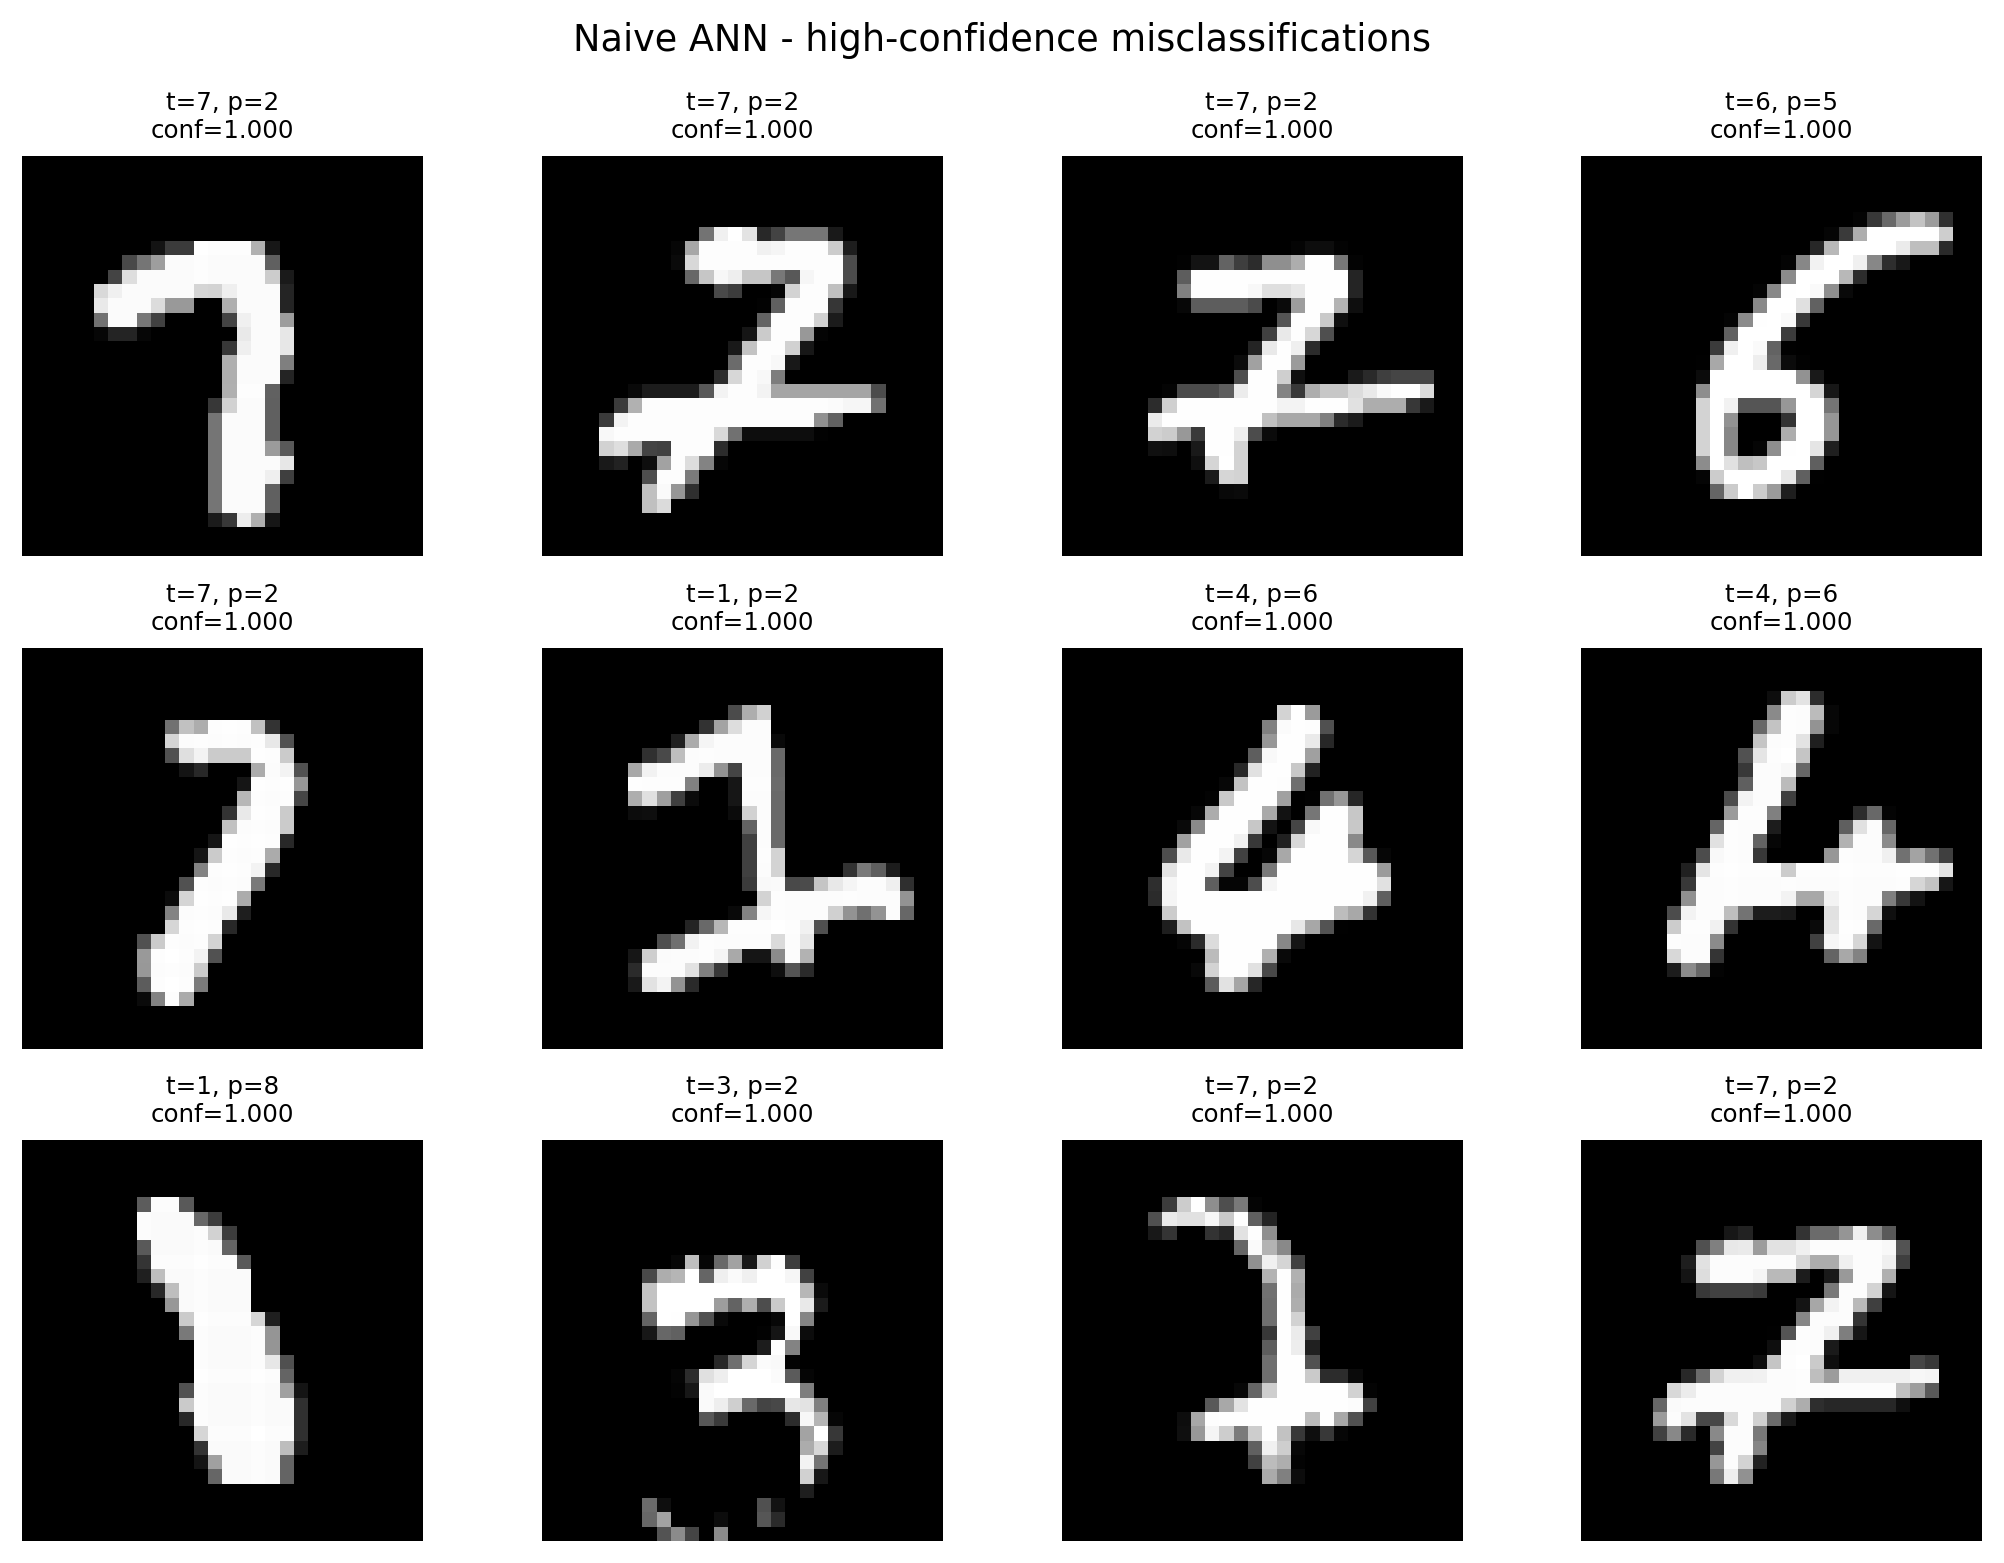
\includegraphics[width=0.92\textwidth]{figures/mnist-models/naive_misclassified_gallery.png}
  \caption{Một số mẫu test bị Naive ANN phân loại sai với độ tin cậy cao.}
  \label{fig:mnist-naive-gallery}
\end{figure}

\begin{figure}[H]
  \centering
  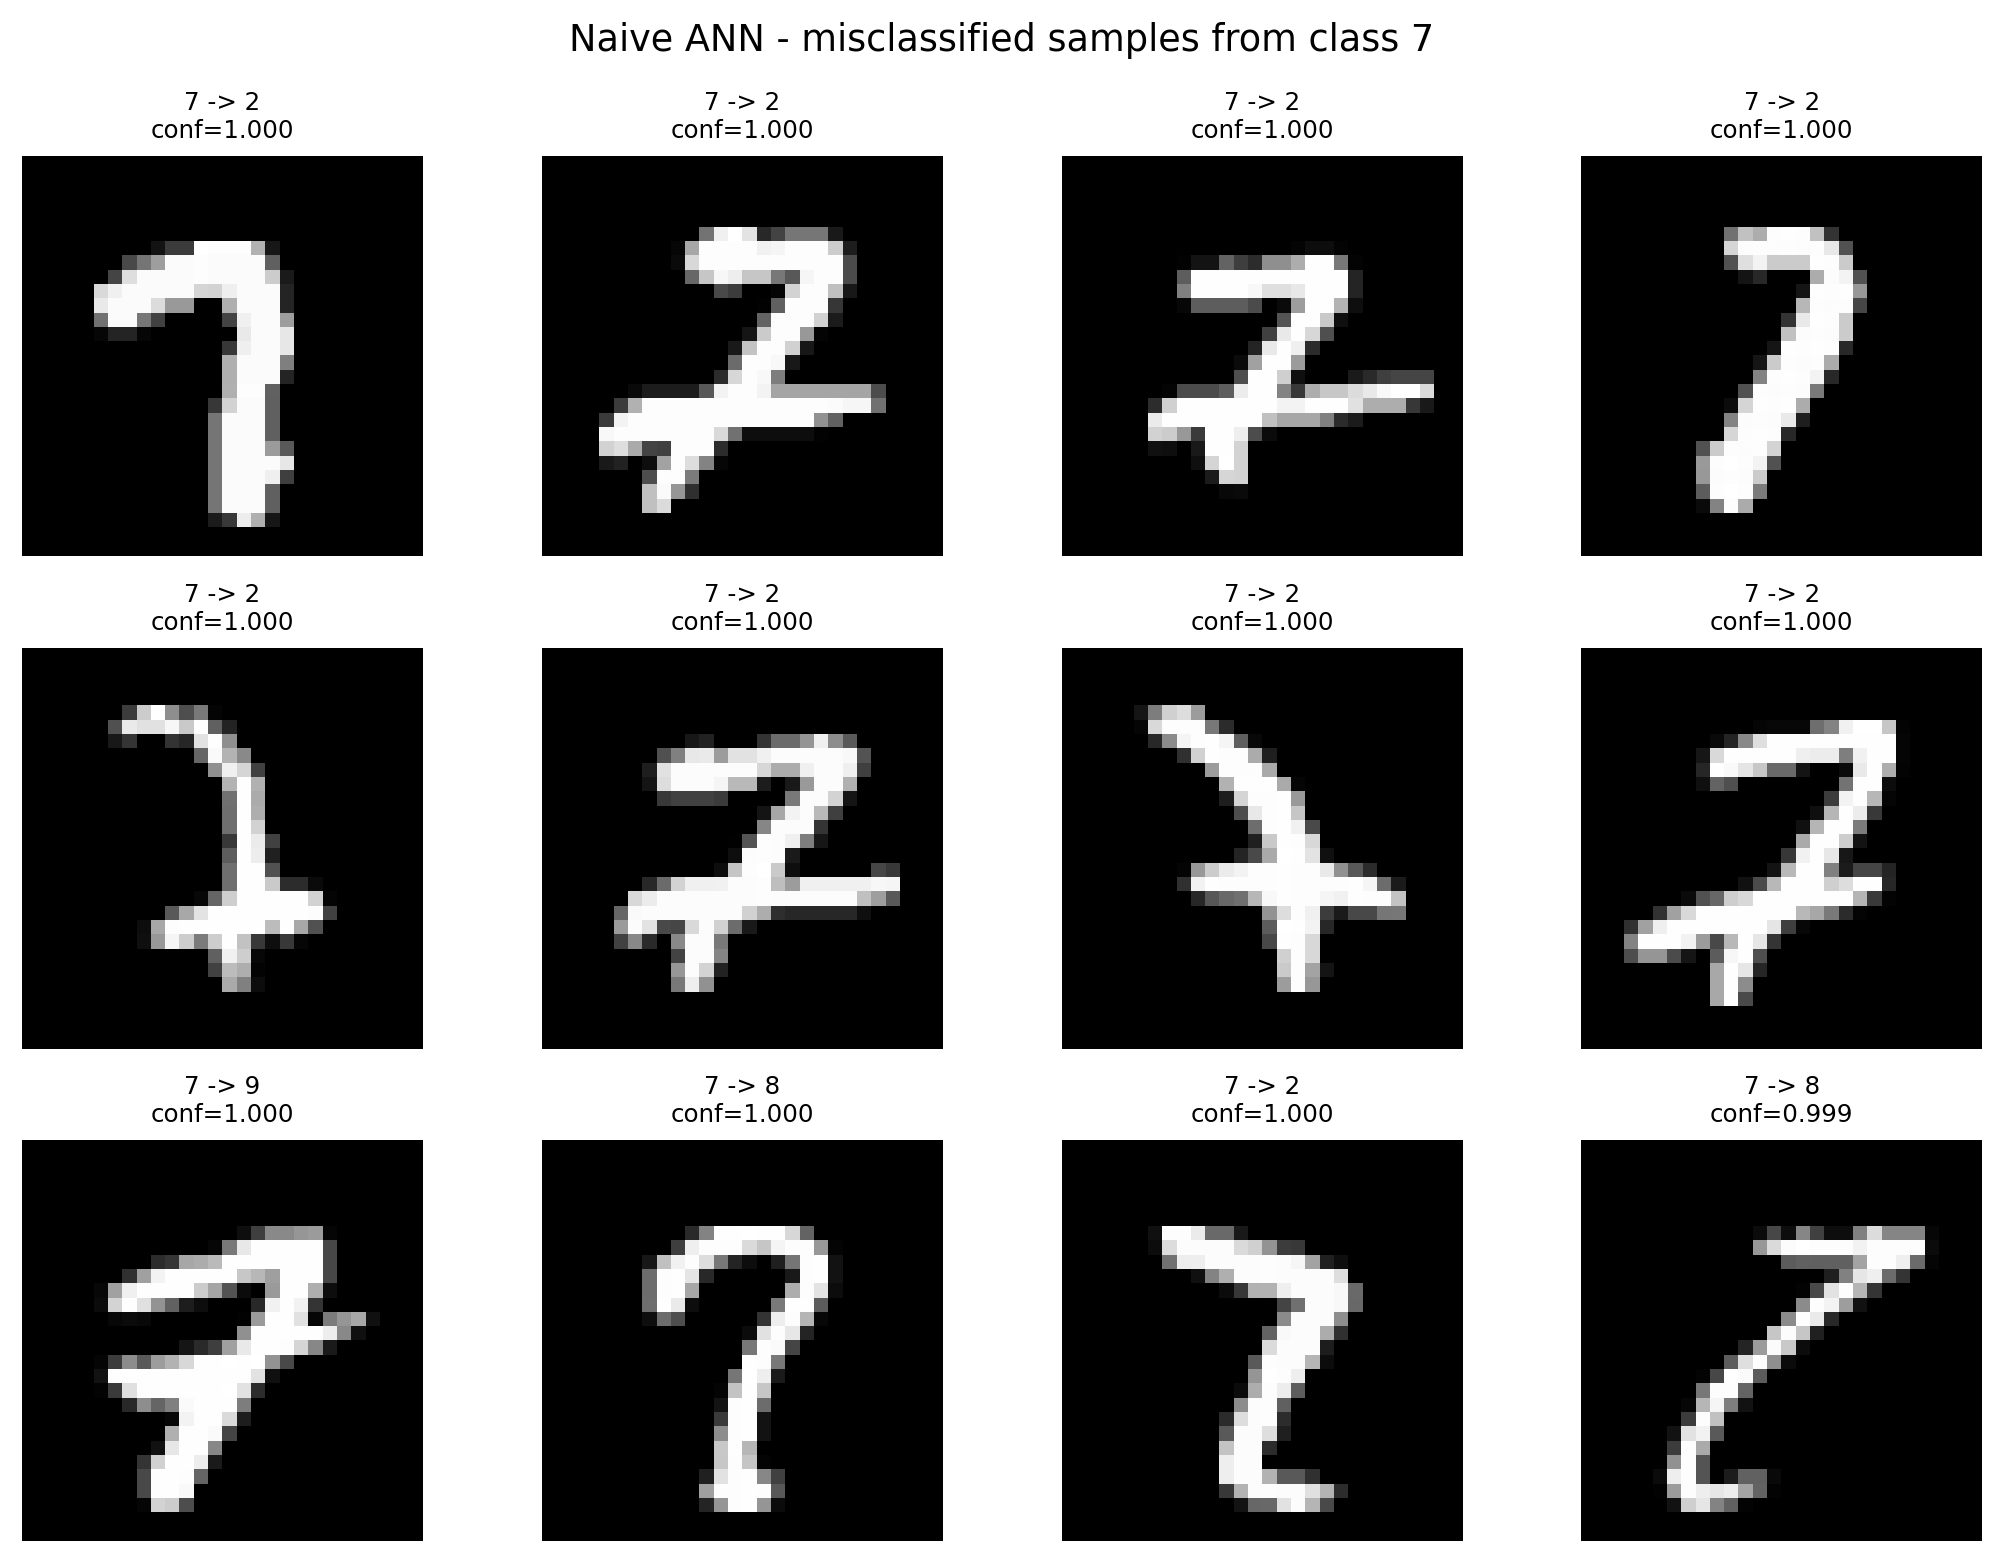
\includegraphics[width=0.92\textwidth]{figures/mnist-models/naive_class7_error_gallery.png}
  \caption{Các mẫu thuộc lớp $7$ bị Naive ANN phân loại sai.}
  \label{fig:mnist-naive-class7-gallery}
\end{figure}

\begin{table}[H]
\centering
\caption{Thống kê lỗi theo từng lớp của Naive ANN trên tập test MNIST}
\label{tab:mnist-naive-error-by-class}
\small
\begin{tabular}{c c c c c}
\toprule
Lớp thật & Số mẫu test & Số dự đoán sai & Tỉ lệ lỗi & Nhầm nhiều nhất \\
\midrule
0 & 980 & 11 & 1.12\% & $0 \rightarrow 6$ (7 mẫu) \\
1 & 1135 & 16 & 1.41\% & $1 \rightarrow 2$ (7 mẫu) \\
2 & 1032 & 13 & 1.26\% & $2 \rightarrow 0$ (2 mẫu) \\
3 & 1010 & 24 & 2.38\% & $3 \rightarrow 2$ (13 mẫu) \\
4 & 982 & 32 & 3.26\% & $4 \rightarrow 9$ (18 mẫu) \\
5 & 892 & 14 & 1.57\% & $5 \rightarrow 3$ (7 mẫu) \\
6 & 958 & 21 & 2.19\% & $6 \rightarrow 5$ (11 mẫu) \\
7 & 1028 & 71 & 6.91\% & $7 \rightarrow 2$ (44 mẫu) \\
8 & 974 & 18 & 1.85\% & $8 \rightarrow 5$ (6 mẫu) \\
9 & 1009 & 34 & 3.37\% & $9 \rightarrow 5$ (9 mẫu) \\
\bottomrule
\end{tabular}
\end{table}


Naive ANN đạt $97.46\%$ test accuracy và có \textit{generalization gap} khoảng $2.25\%$, lớn nhất trong bốn biến thể. Confusion matrix của mô hình cho thấy lỗi không phân bố ngẫu nhiên mà tập trung rất mạnh vào các cặp có hình thái gần nhau, nổi bật nhất là $7 \rightarrow 2$, $4 \rightarrow 9$, $3 \rightarrow 2$ và $6 \rightarrow 5$. Các lớp khó nhất là $7$, $9$ và $4$. Tập hợp các mẫu sai cũng cho thấy những ảnh bị nhầm thường có xu hướng nghiêng, lệch tâm hoặc có stroke chồng lấn về cấu trúc, đúng với insight từ EDA.

Bảng thống kê lỗi theo lớp ở ngay trên làm rõ hơn bản chất của các lỗi này. Lớp $7$ có tỉ lệ lỗi cao nhất, gần $7\%$, và riêng cặp $7 \rightarrow 2$ đã chiếm $44$ mẫu sai. Hai lớp $4$ và $9$ cũng có tỉ lệ lỗi cao vì chúng phụ thuộc mạnh vào vị trí giao nhau giữa các stroke và độ nghiêng của nét dọc. Hình hiển thị riêng cho lớp $7$ cho thấy rõ điểm chung của các mẫu bị nhầm: nét ngang phía trên thường ngắn hoặc cong, thân dọc bị nghiêng và phần chân dưới tạo thành một móc ngang, khiến hình tổng thể gần với số $2$; ở một số mẫu khác, phần đầu cong hơn và phần thân kéo dài xuống dưới khiến mô hình còn nhầm sang $8$ hoặc $9$. Nhóm lỗi $3 \rightarrow 2$, $4 \rightarrow 9$, $6 \rightarrow 5$, $7 \rightarrow 2$ và $9 \rightarrow 5$ đều có một đặc điểm chung: raw pixel giữ được cường độ sáng, nhưng biểu diễn rất kém thông tin về hướng nét và bố cục hình học.

Từ kết quả này, có thể thấy raw pixel phẳng là chưa đủ. Vấn đề không phải ANN không học được MNIST, mà là ANN đang phải tự học quá nhiều thông tin hình học và hướng nét từ biểu diễn đầu vào còn quá thô. Vì vậy, bước cải tiến kế tiếp hợp lý nhất là chuẩn hóa hình học bằng \textit{deslant + recenter} để giảm lệch tâm và độ nghiêng, đồng thời thêm HOG để đưa thông tin gradient vào mô hình ngay từ đầu. Nói cách khác, biến thể kế tiếp không được thiết kế ngẫu nhiên, mà được sinh ra trực tiếp từ đúng nhóm lỗi mà baseline vừa bộc lộ.

\subsection{Single-branch ANN}

Trong biến thể này, phần HOG cần được nêu rõ vì đây là nguồn tạo ra phần lớn thông tin hình học mới so với baseline. Với cấu hình \textit{orientations} $= 9$, \textit{pixels per cell} $= (4,4)$, \textit{cells per block} $= (2,2)$, ảnh $28 \times 28$ được chia thành lưới $7 \times 7$ cell. Khi block $2 \times 2$ trượt trên lưới này, số block theo mỗi chiều là $7 - 2 + 1 = 6$, nên tổng cộng có $6 \times 6 = 36$ block. Mỗi block chứa $2 \times 2$ cell và mỗi cell có $9$ bins hướng gradient, do đó một block sinh ra $2 \times 2 \times 9 = 36$ đặc trưng. Tổng số chiều HOG là $36 \times 36 = 1296$. Khi ghép với raw pixel $784$ chiều, đầu vào chung của single-branch trở thành vector $2080 = 784 + 1296$ chiều.
Single-branch ANN là bước cải tiến trực tiếp từ baseline. Ảnh trước hết được đưa qua \textit{deslant} để giảm biến thiên nghiêng và \textit{recenter} để đưa chữ số về vị trí ổn định hơn trong khung hình. Sau đó raw pixel $784$ chiều được giữ lại và ghép với vector HOG $1296$ chiều thành đầu vào chung $2080$ chiều. MLP phía sau có dạng $2080 \rightarrow 1024 \rightarrow 512 \rightarrow 256 \rightarrow 10$. Kích thước $1024$ ở tầng đầu được giữ đủ lớn để không làm mất thông tin khi raw pixel và HOG vừa mới được ghép lại, sau đó nén dần về $512$ rồi $256$ để đưa sang lớp phân loại cuối. BatchNorm được thêm để ổn định kích hoạt ở các tầng ẩn, còn Dropout được dùng để tăng regularization và giảm chênh lệch giữa train và test.

Nếu viết chặt chẽ hơn về vai trò của hai kỹ thuật này, BatchNorm và Dropout không giải quyết cùng một bài toán. BatchNorm chủ yếu giúp ổn định kích hoạt và làm quá trình tối ưu bớt nhạy với chênh lệch phân bố giữa các chiều đặc trưng, điều này đặc biệt quan trọng vì đầu vào $2080$ chiều được ghép từ raw pixel và HOG. Dropout thì nhắm vào regularization: nó buộc mạng không được phụ thuộc quá mạnh vào một nhóm neuron cụ thể trong lúc train. Ở đây, Dropout $(p=0.25)$ được đặt sau mỗi tầng ẩn để giảm độ nhạy của các lớp fully-connected có khá nhiều tham số. Nói ngắn gọn, BatchNorm chủ yếu nhắm về ổn định tối ưu và scale kích hoạt, còn Dropout nhắm về regularization; hai thứ được dùng đồng thời vì chúng bổ sung nhau thay vì thay thế nhau.

\begin{figure}[H]
  \centering
  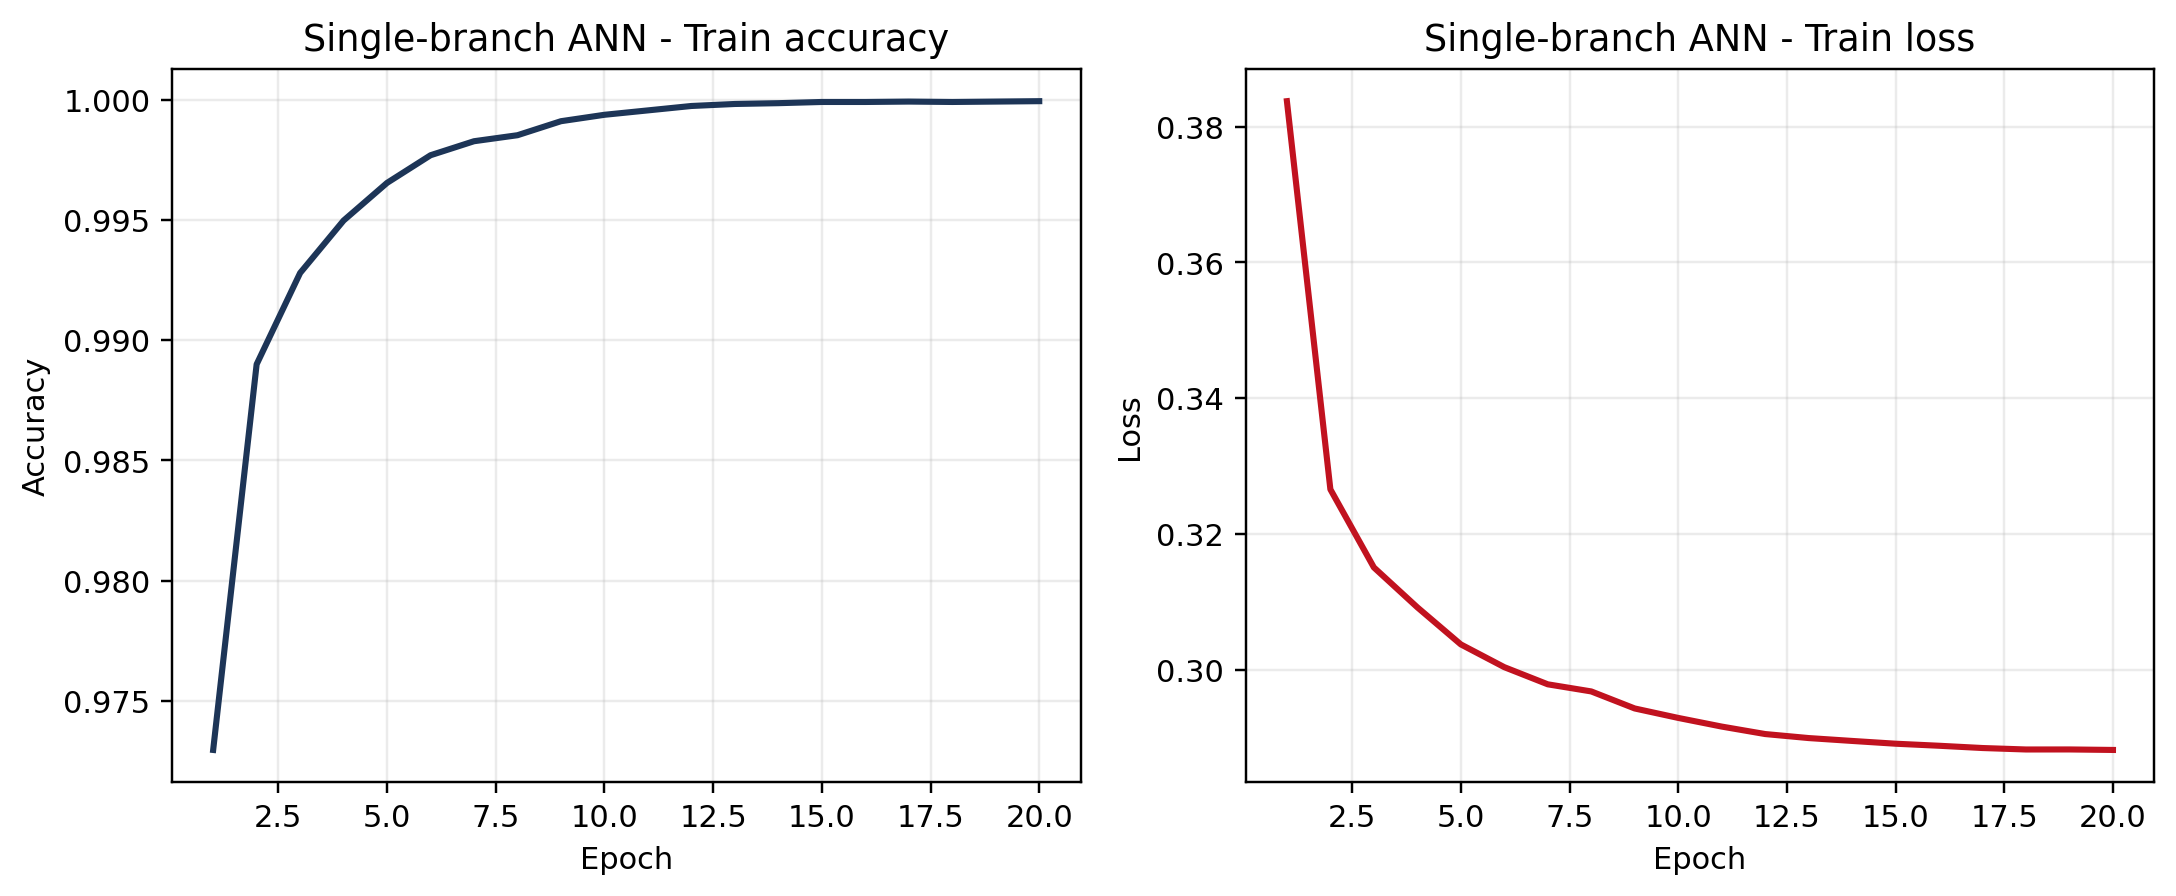
\includegraphics[width=0.92\textwidth]{figures/mnist-models/single_branch_training_curves.png}
  \caption{Diễn biến train accuracy và train loss của Single-branch ANN.}
  \label{fig:mnist-single-training}
\end{figure}

\begin{figure}[H]
  \centering
  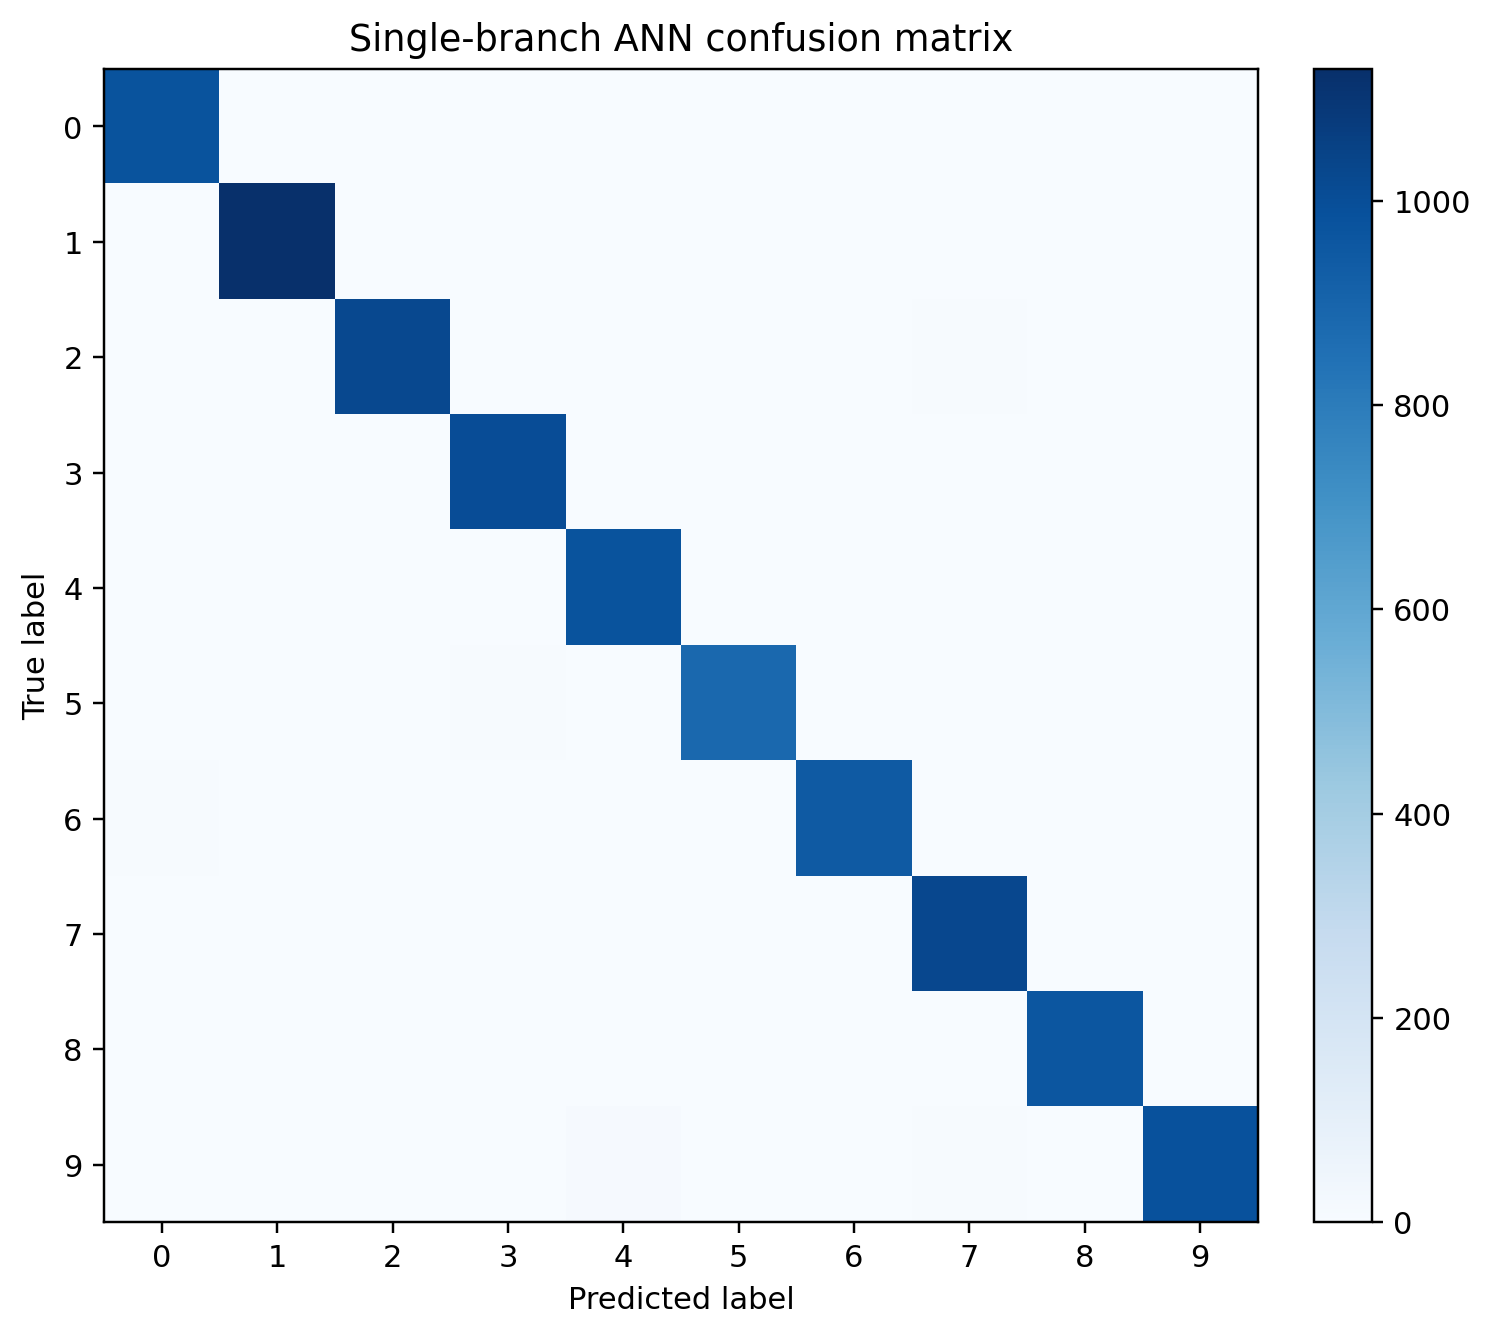
\includegraphics[width=0.72\textwidth]{figures/mnist-models/single_branch_confusion_matrix.png}
  \caption{Confusion matrix của Single-branch ANN trên tập test MNIST.}
  \label{fig:mnist-single-confusion}
\end{figure}

\begin{figure}[H]
  \centering
  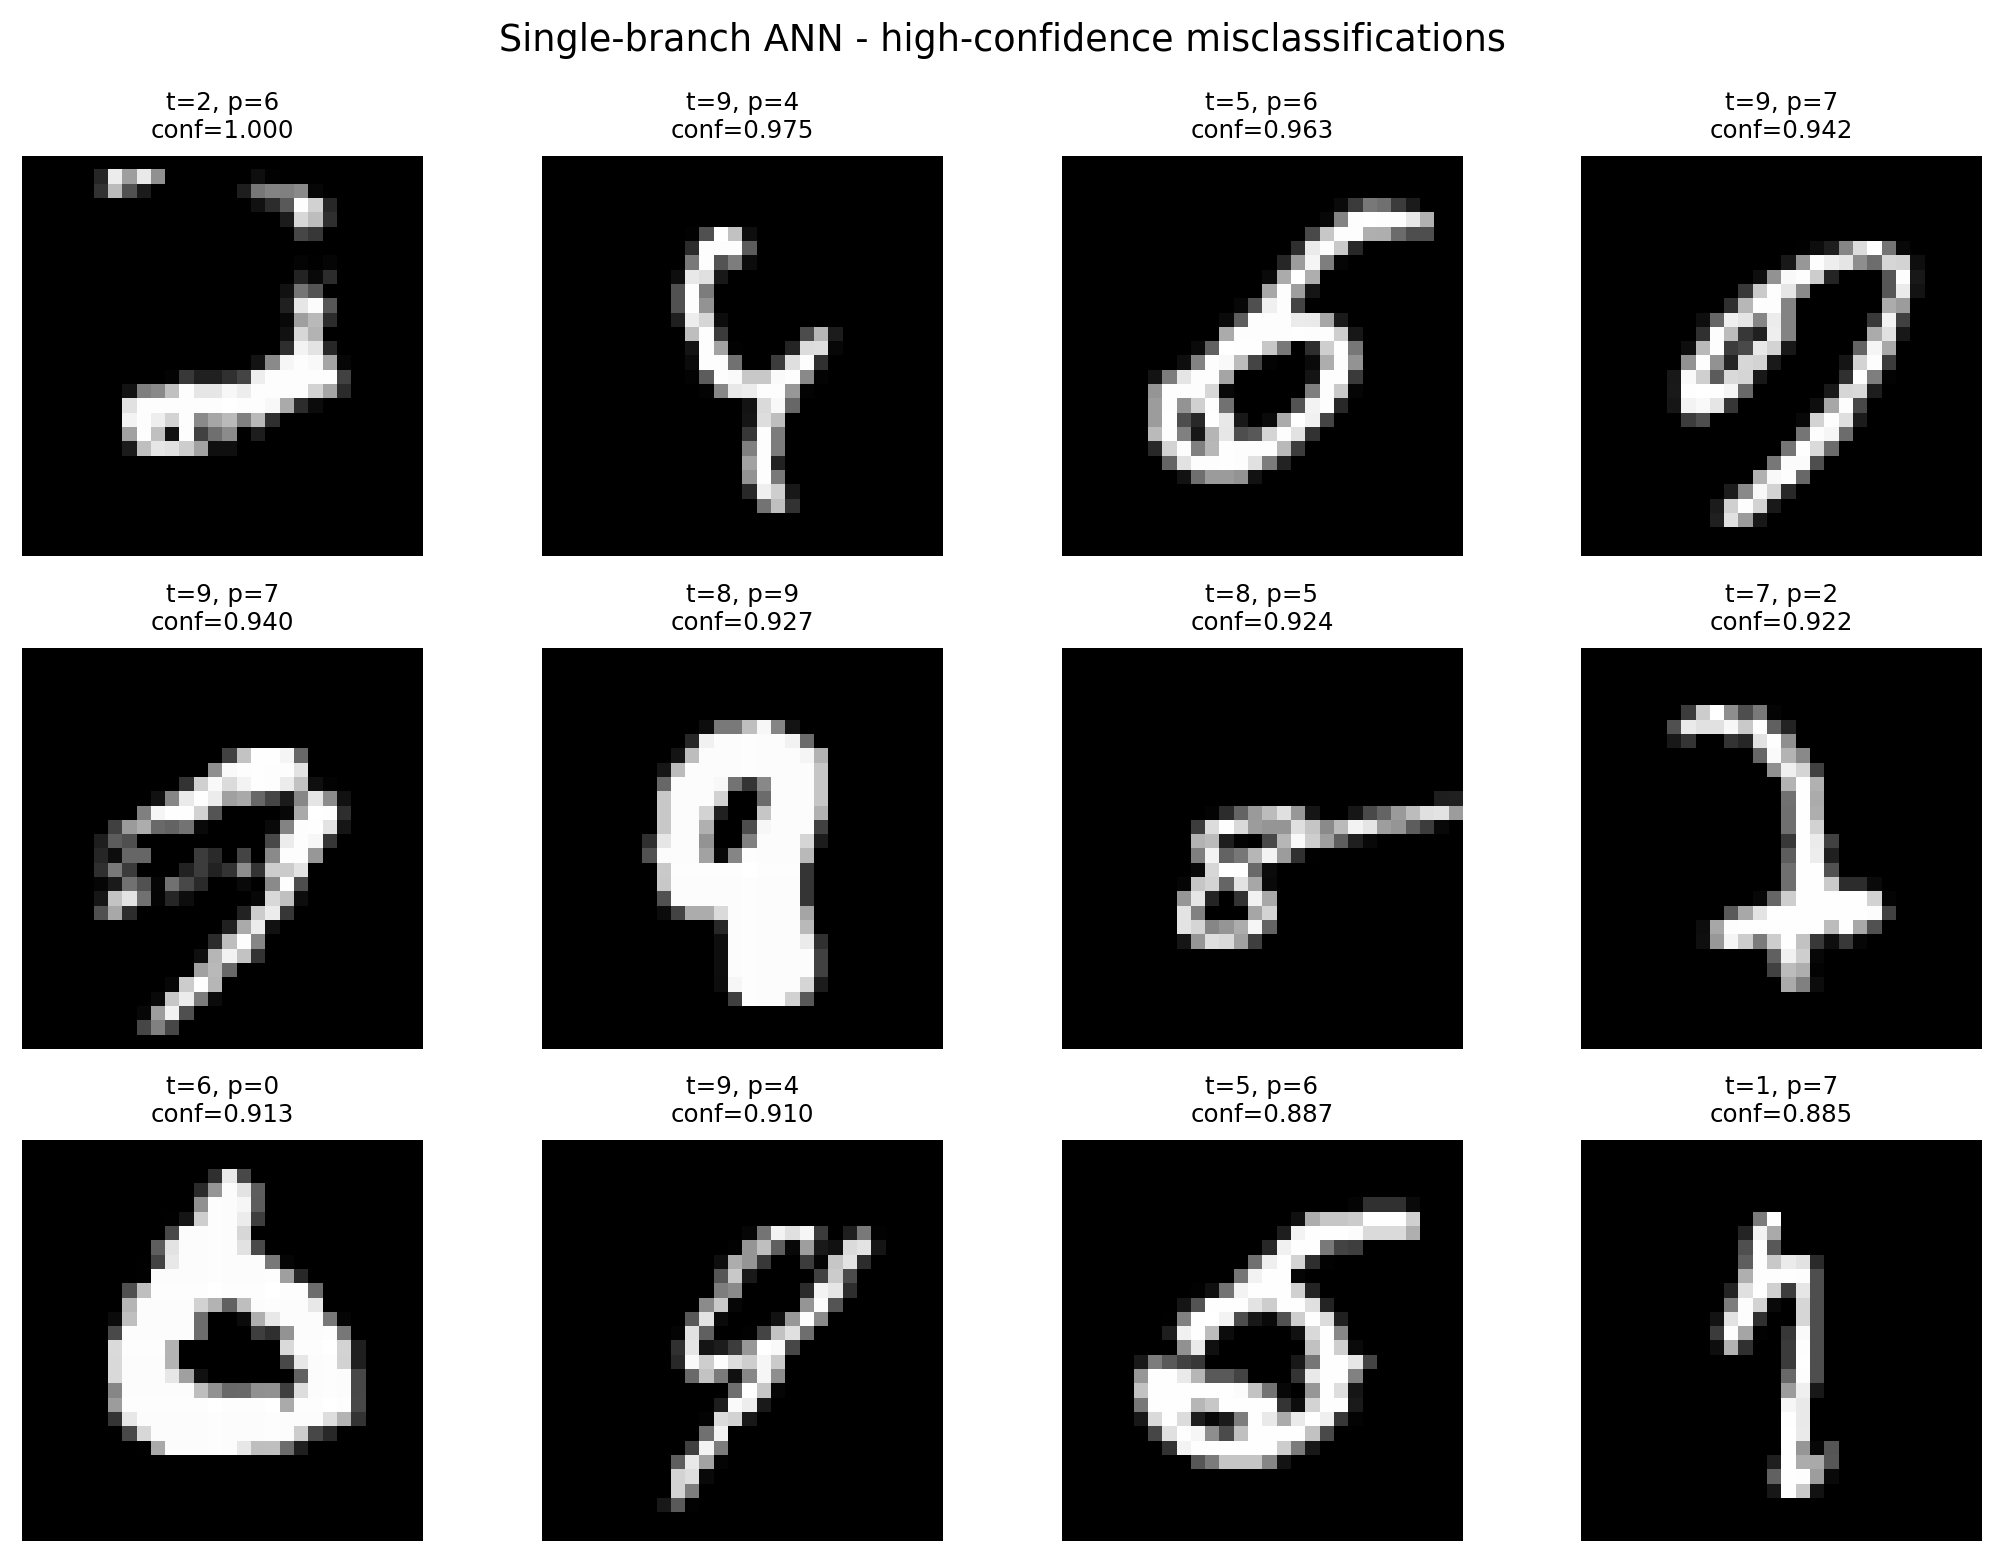
\includegraphics[width=0.92\textwidth]{figures/mnist-models/single_branch_misclassified_gallery.png}
  \caption{Một số mẫu test bị Single-branch ANN phân loại sai với độ tin cậy cao.}
  \label{fig:mnist-single-gallery}
\end{figure}

Single-branch ANN đạt $99.14\%$ test accuracy và giảm \textit{generalization gap} xuống khoảng $0.86\%$. Đây là bước nhảy lớn nhất trong toàn bộ quá trình thử nghiệm, cho thấy tiền xử lý và đặc trưng hóa giải quyết đúng nút thắt của baseline. Các cặp nhầm lẫn lớn nhất giảm mạnh; lỗi còn lại chủ yếu tập trung ở các chữ số $9$, $6$, $5$ và $8$, nổi bật nhất là $9 \rightarrow 4$ và $9 \rightarrow 7$. Gallery các mẫu sai cho thấy ảnh bị nhầm lúc này không còn lệch tâm hay nghiêng quá mạnh như baseline, mà chủ yếu khó ở mức hình thái stroke cục bộ.

Sau bước này, giả thuyết tự nhiên tiếp theo là: nếu các lỗi còn lại nằm ở chi tiết cục bộ của nét viết, có thể tăng thêm đa dạng nét viết trong tập train bằng augmentation cục bộ, thay vì tiếp tục thay đổi mạnh kiến trúc.

\subsection{Single-branch + local augmentation}

Biến thể này giữ nguyên kiến trúc single-branch và toàn bộ pipeline \textit{deslant + recenter + HOG + BatchNorm + Dropout}, nhưng bổ sung thêm augmentation cục bộ. Thay vì tăng mạnh các phép affine toàn cục, mô hình chỉ thêm \textit{elastic distortion} nhẹ để mô phỏng độ cong cục bộ của nét viết và \textit{stroke jitter} nhẹ để mô phỏng thay đổi bề dày nét. Ý tưởng của biến thể này là sau khi \textit{deslant} và \textit{recenter} đã xử lý phần lớn biến thiên hình học toàn cục, augmentation nên tập trung vào phần biến thiên nét viết mà tiền xử lý chưa giải quyết hết.

\begin{figure}[H]
  \centering
  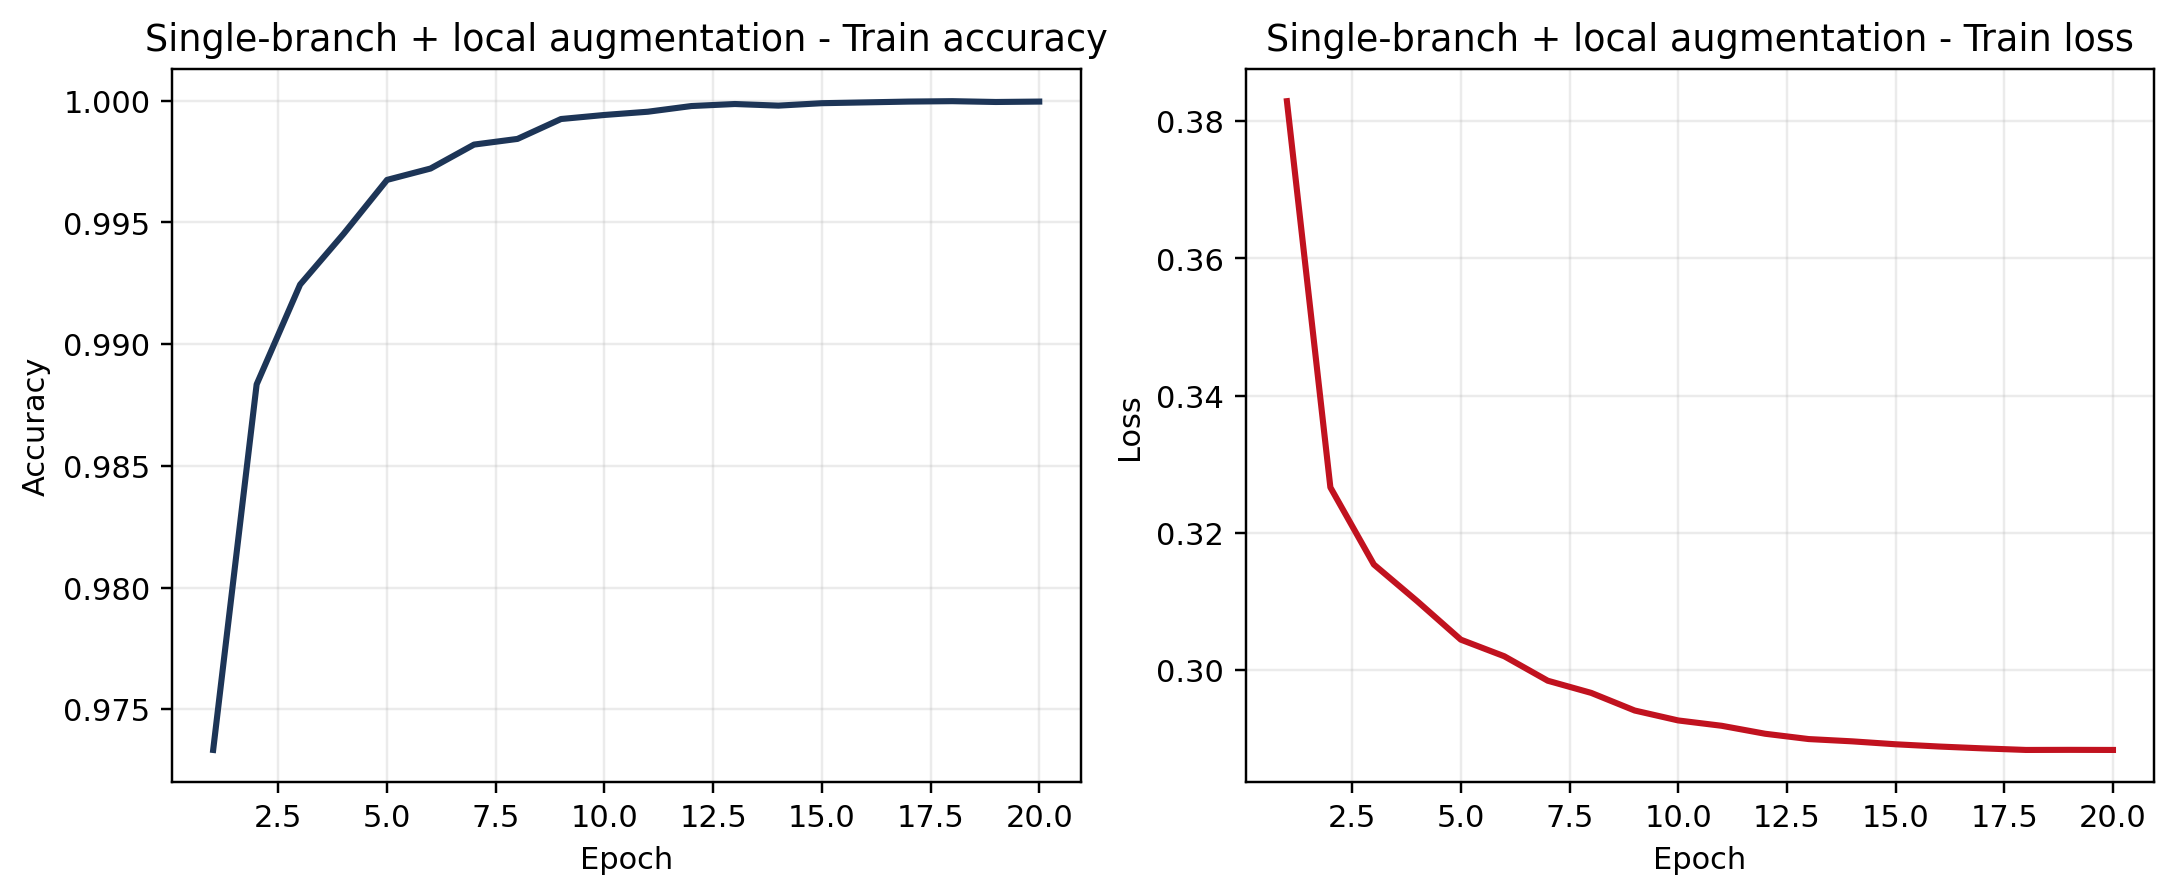
\includegraphics[width=0.92\textwidth]{figures/mnist-models/single_branch_augmented_training_curves.png}
  \caption{Diễn biến train accuracy và train loss của Single-branch ANN với local augmentation.}
  \label{fig:mnist-single-aug-training}
\end{figure}

\begin{figure}[H]
  \centering
  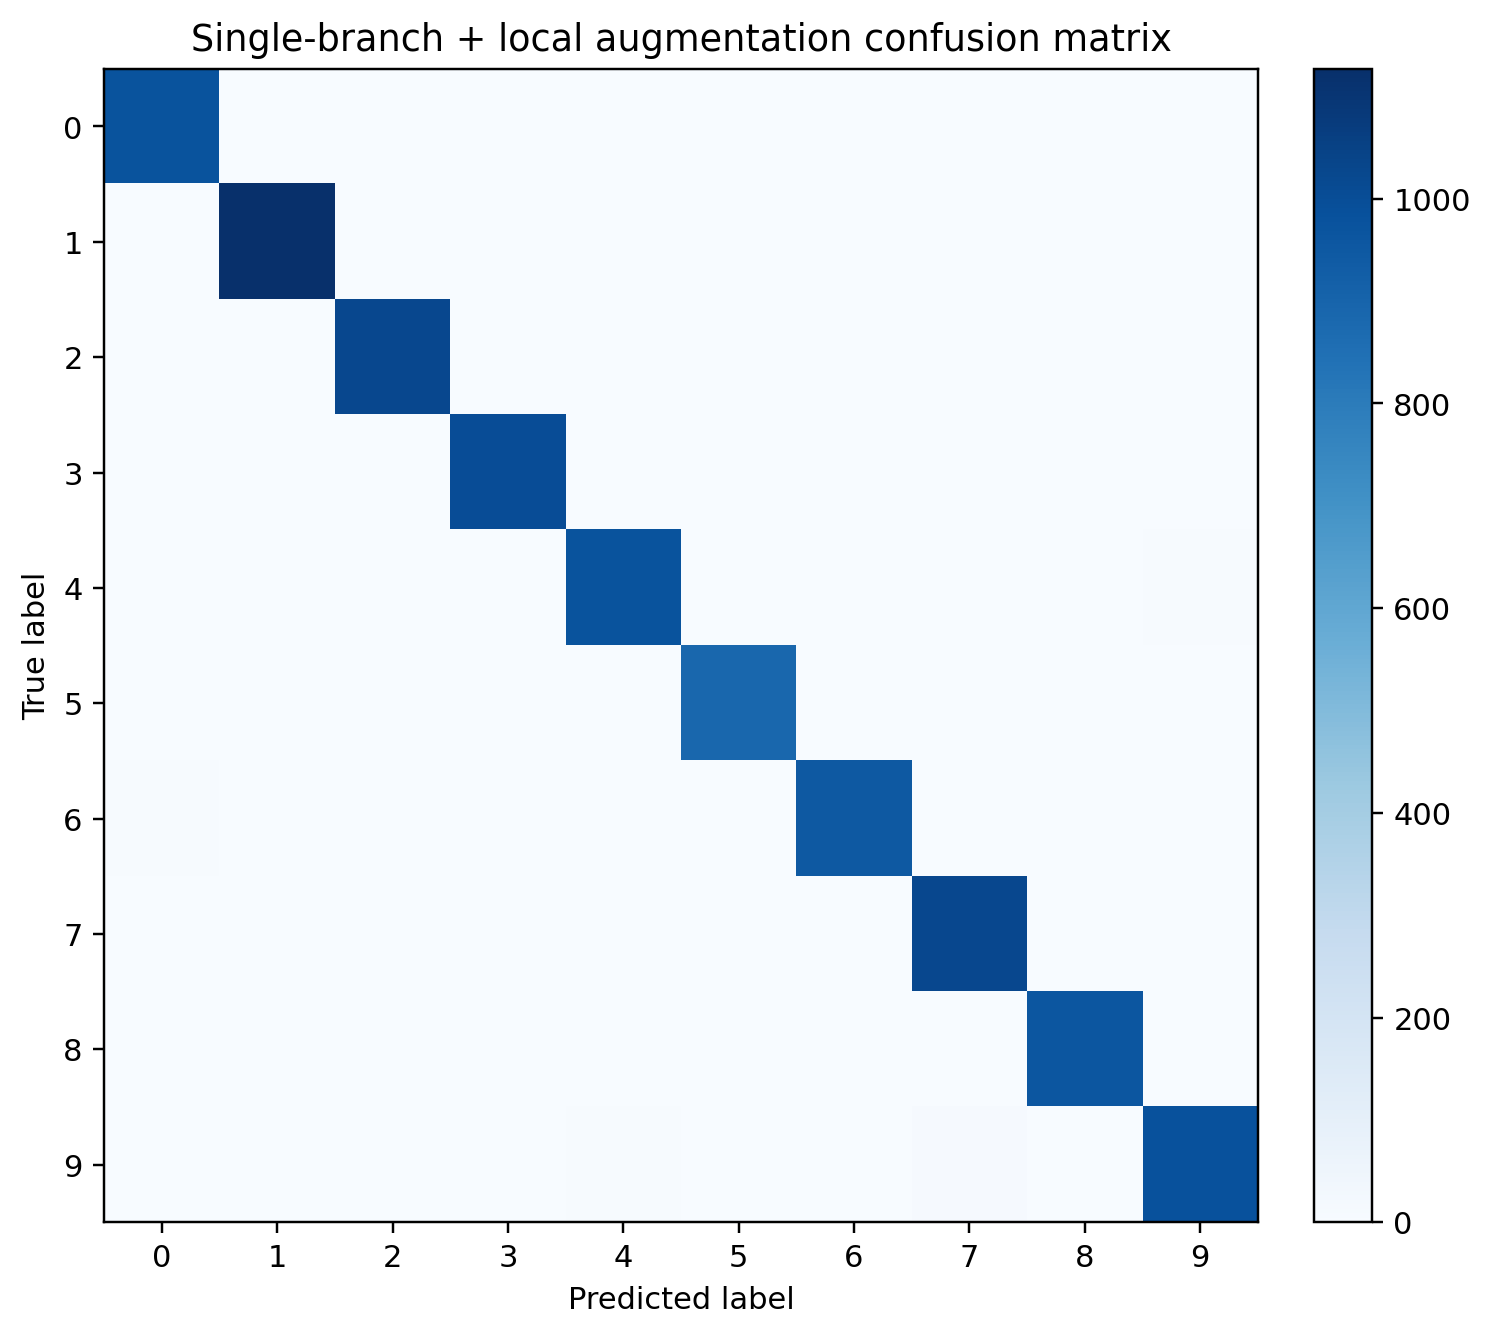
\includegraphics[width=0.72\textwidth]{figures/mnist-models/single_branch_augmented_confusion_matrix.png}
  \caption{Confusion matrix của Single-branch ANN với local augmentation trên tập test MNIST.}
  \label{fig:mnist-single-aug-confusion}
\end{figure}

\begin{figure}[H]
  \centering
  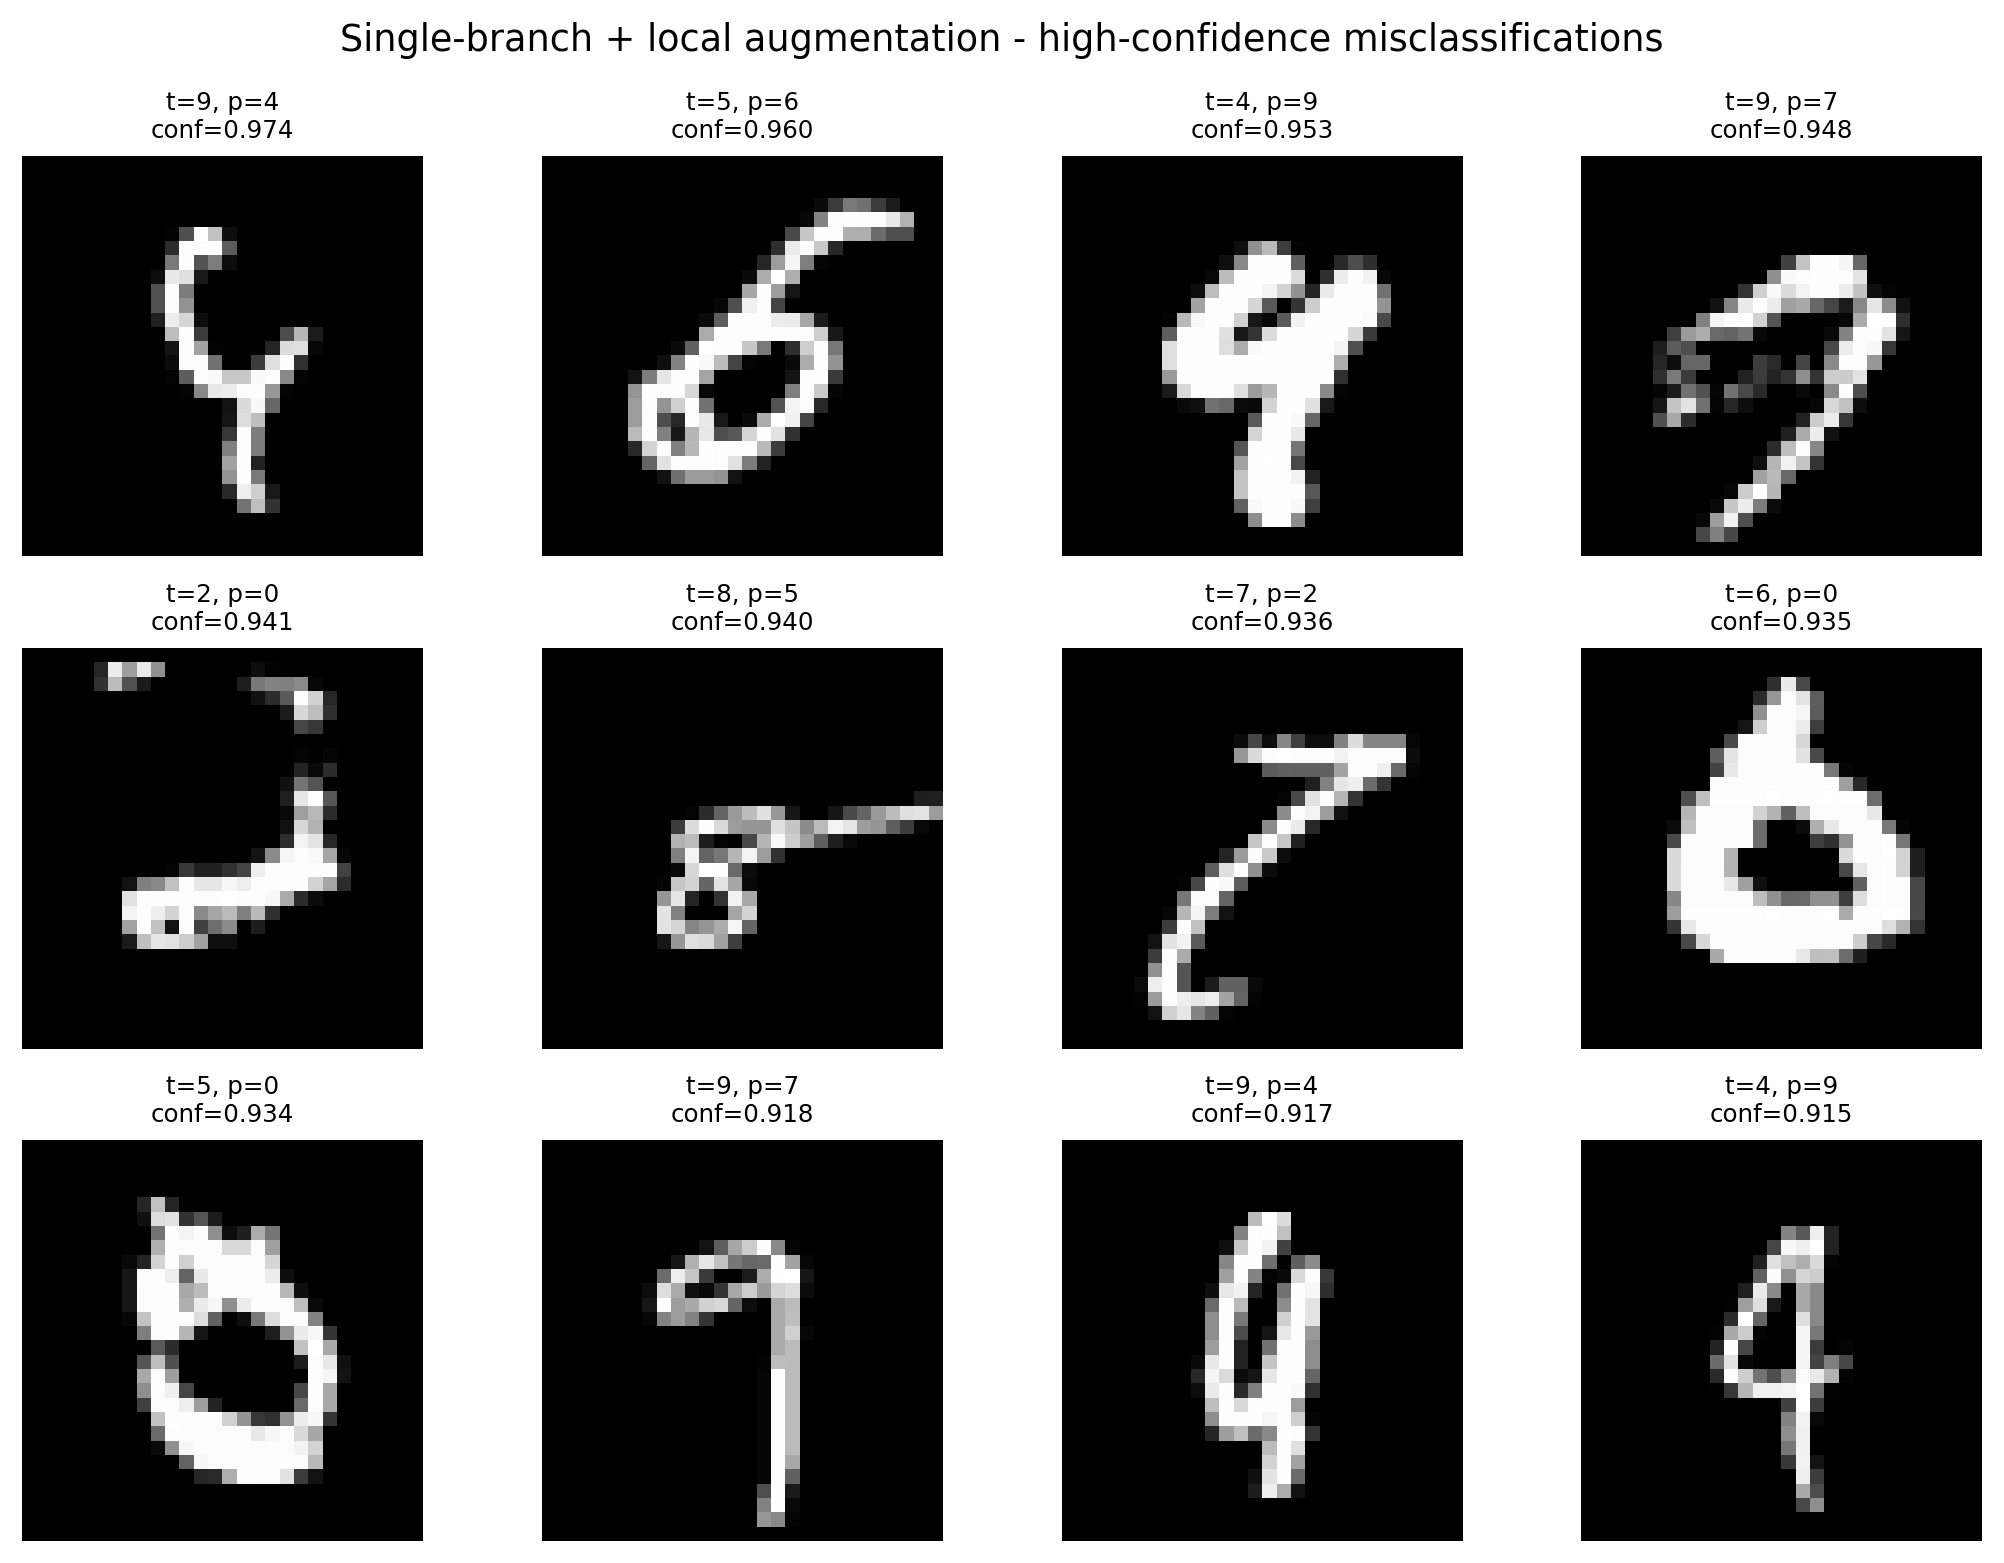
\includegraphics[width=0.92\textwidth]{figures/mnist-models/single_branch_augmented_misclassified_gallery.png}
  \caption{Một số mẫu test bị Single-branch ANN với local augmentation phân loại sai.}
  \label{fig:mnist-single-aug-gallery}
\end{figure}

Biến thể này đạt $99.11\%$ test accuracy, gần như tương đương với single-branch gốc nhưng không vượt lên trên. Các lỗi lớn nhất vẫn xoay quanh chữ số $9$, đặc biệt là $9 \rightarrow 7$ và $9 \rightarrow 4$, trong khi lớp khó nhất vẫn là $9$ rồi tới $6$ và $8$. Nói cách khác, augmentation cục bộ làm mô hình bền hơn với biến thiên nét viết, nhưng không tạo ra bước nhảy mới về mặt tổng thể.

Từ đây xuất hiện một giả thuyết khác: có thể bottleneck không còn nằm ở độ đa dạng dữ liệu nữa, mà nằm ở cách raw pixel và HOG đang bị ghép quá sớm thành một vector chung. Nếu đúng vậy, nên thử cho mỗi loại đầu vào đi qua một nhánh riêng trước khi hợp nhất ở tầng sâu hơn.

\subsection{Two-branch ANN}

Two-branch ANN dùng cùng đầu vào và cùng pipeline tiền xử lý như single-branch, nhưng thay vì ghép raw pixel và HOG ngay từ đầu, mô hình tách chúng thành hai nhánh học riêng. Nhánh raw có dạng $784 \rightarrow 512 \rightarrow 256$, còn nhánh HOG có dạng $1296 \rightarrow 768 \rightarrow 256$. Nhánh HOG được cấp tầng đầu rộng hơn vì đầu vào của nó có số chiều lớn hơn và mang nhiều thông tin cấu trúc hơn raw pixel. Sau khi mỗi nhánh đã nén về $256$ chiều, hai vector được ghép lại thành $512$ chiều rồi đi qua head cuối $512 \rightarrow 256 \rightarrow 10$. Thiết kế này giúp mô hình học riêng hai kiểu biểu diễn trước khi hợp nhất chúng ở tầng sâu hơn.

\begin{figure}[H]
  \centering
  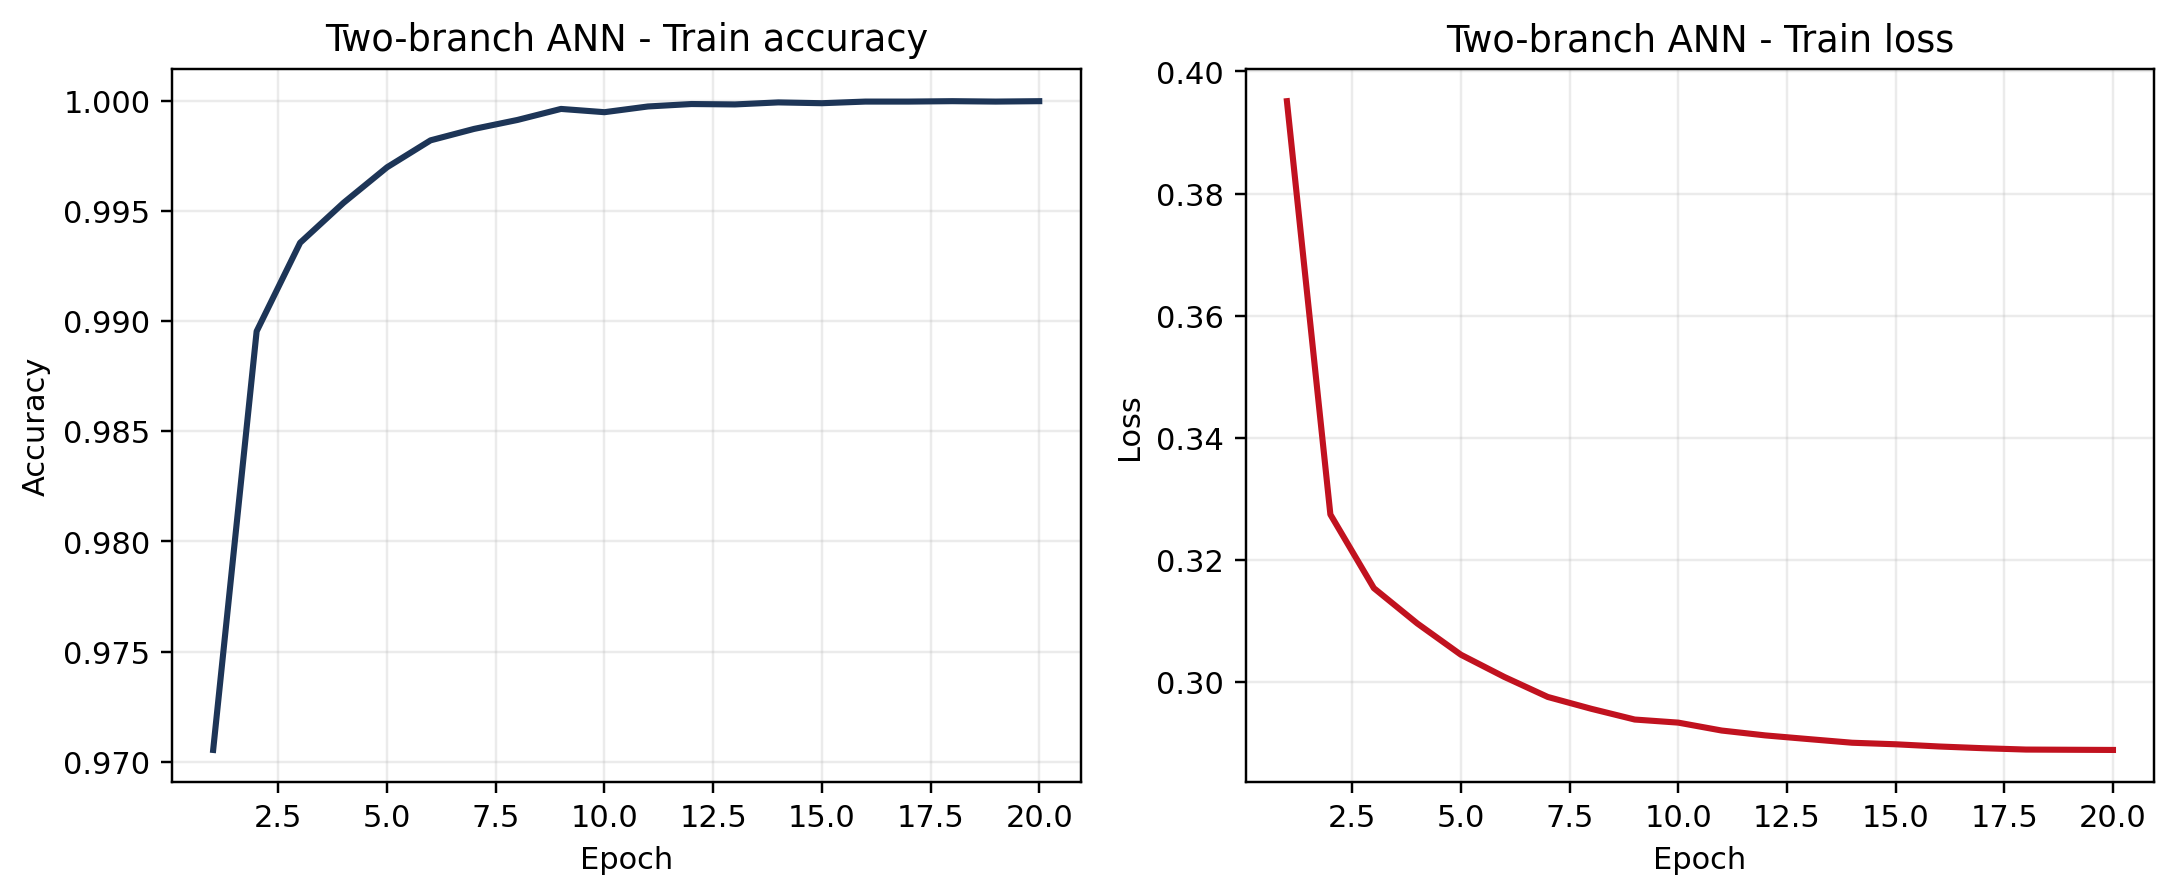
\includegraphics[width=0.92\textwidth]{figures/mnist-models/two_branch_training_curves.png}
  \caption{Diễn biến train accuracy và train loss của Two-branch ANN.}
  \label{fig:mnist-two-training}
\end{figure}

\begin{figure}[H]
  \centering
  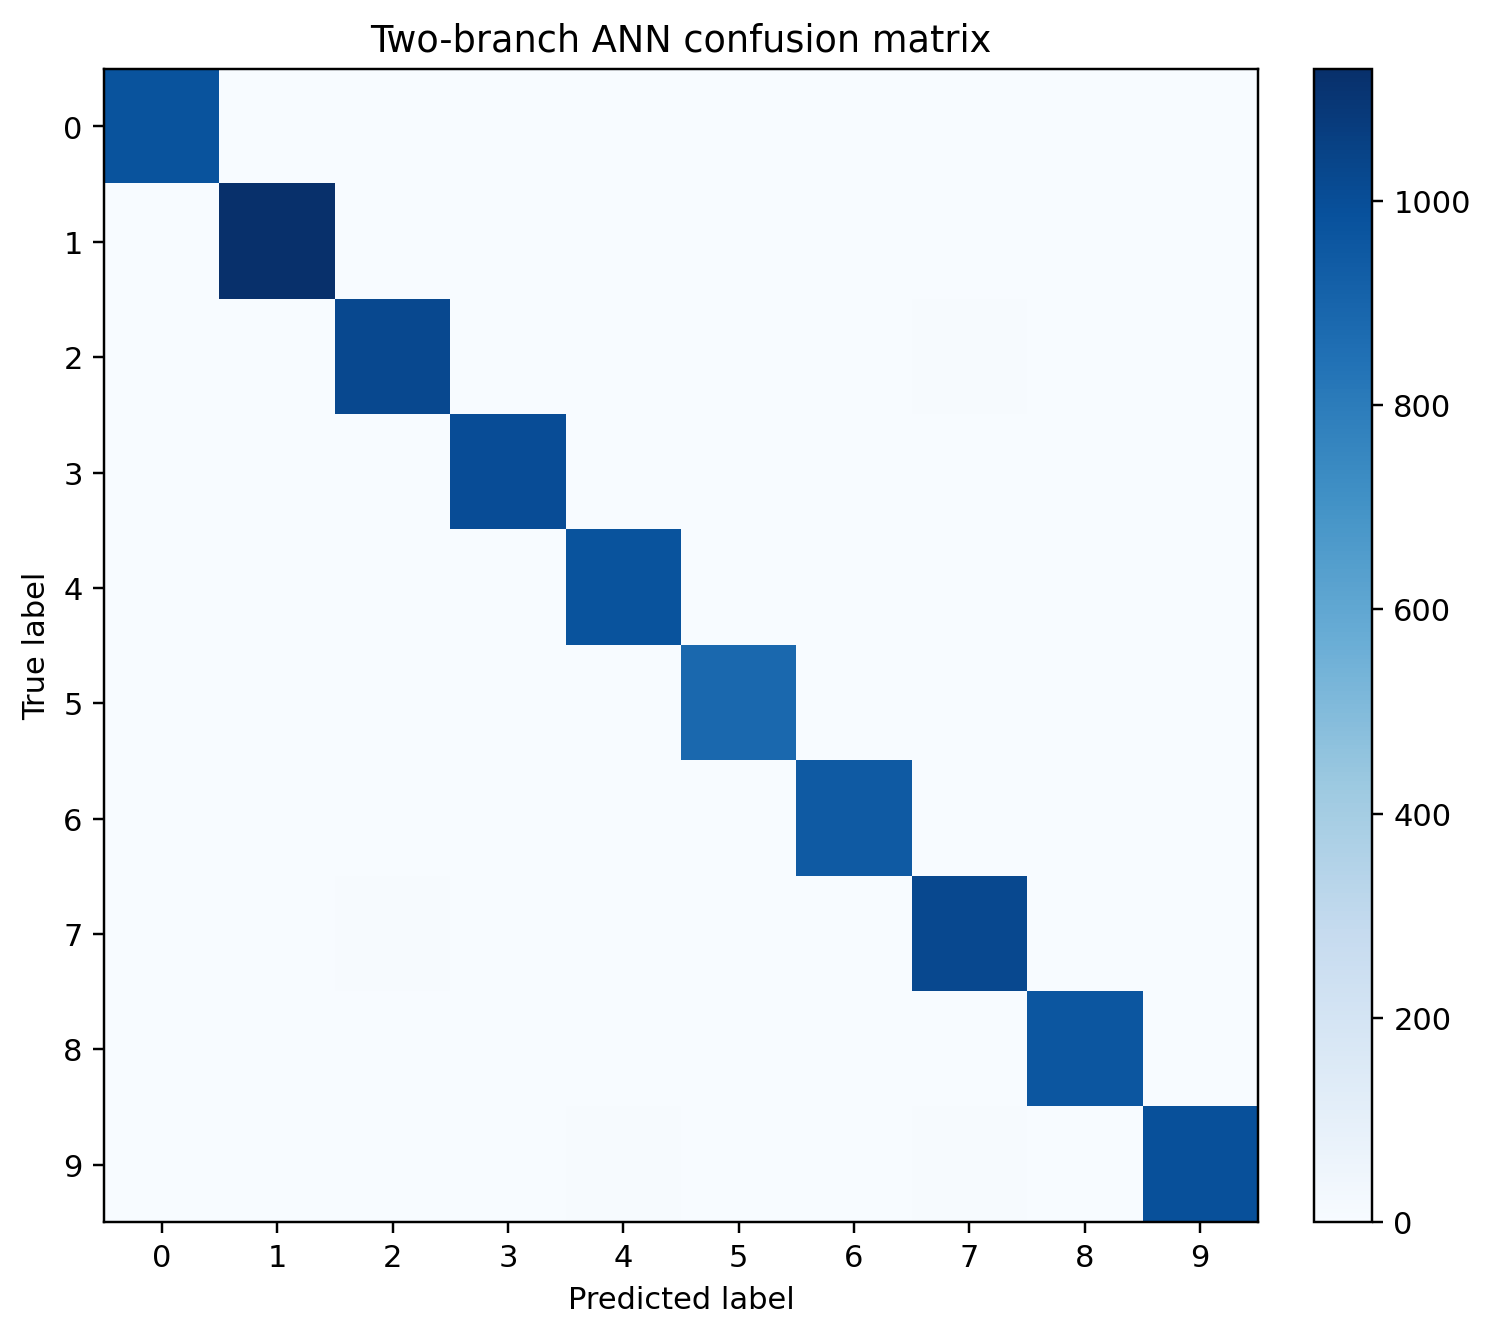
\includegraphics[width=0.72\textwidth]{figures/mnist-models/two_branch_confusion_matrix.png}
  \caption{Confusion matrix của Two-branch ANN trên tập test MNIST.}
  \label{fig:mnist-two-confusion}
\end{figure}

\begin{figure}[H]
  \centering
  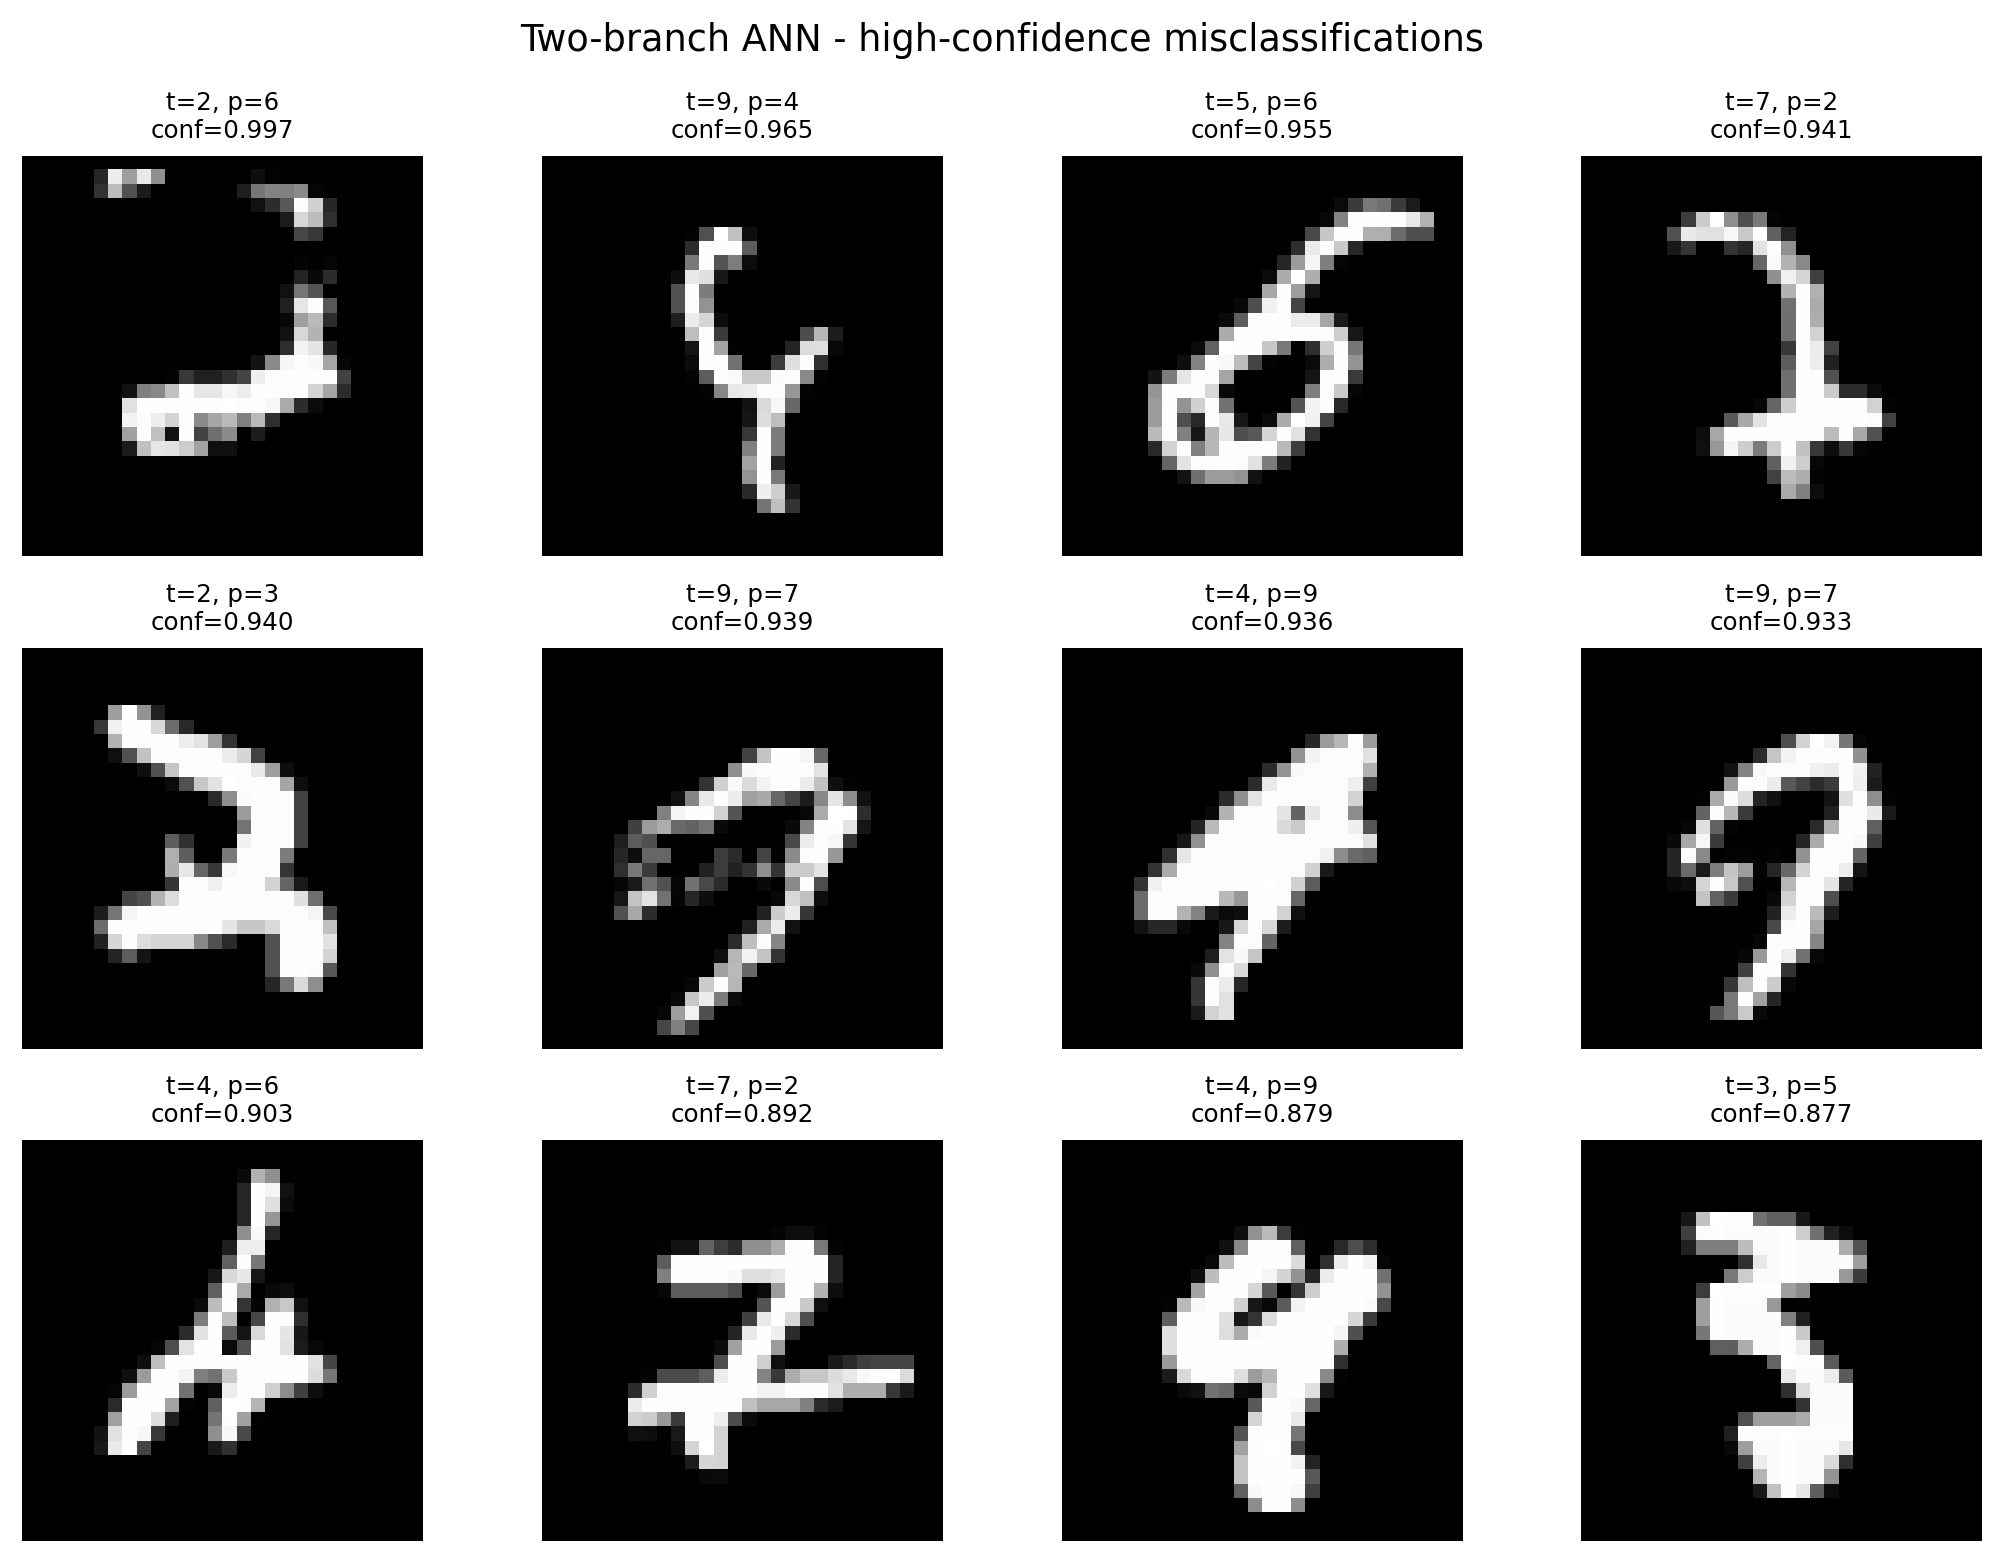
\includegraphics[width=0.92\textwidth]{figures/mnist-models/two_branch_misclassified_gallery.png}
  \caption{Một số mẫu test bị Two-branch ANN phân loại sai với độ tin cậy cao.}
  \label{fig:mnist-two-gallery}
\end{figure}

Two-branch ANN đạt $99.10\%$ test accuracy và có \textit{generalization gap} khoảng $0.90\%$. Kết quả này vẫn rất mạnh, nhưng không vượt được single-branch gốc trong lượt chạy hiện tại. Lỗi còn lại vẫn tập trung ở các cặp hình thái khó như $9 \rightarrow 4$, $9 \rightarrow 7$, $7 \leftrightarrow 2$ và $5 \rightarrow 3$. Điều này cho thấy giả thuyết “tách hai nhánh sẽ luôn tốt hơn” không phải lúc nào cũng đúng; sau khi dữ liệu đã được chuẩn hóa hình học tốt và HOG đã đủ mạnh, bottleneck còn lại không nhất thiết nằm ở kiến trúc hợp nhất đặc trưng.

\section{Tổng hợp kết quả và nhận xét}

\begin{table}[H]
\centering
\caption{Thông số đầu vào và kiến trúc của bốn biến thể ANN}
\label{tab:mnist-ann-architecture-details}
\small
\begin{tabularx}{\textwidth}{>{\raggedright\arraybackslash}p{2.8cm} >{\raggedright\arraybackslash}p{2.8cm} >{\raggedright\arraybackslash}X >{\raggedright\arraybackslash}p{3.0cm}}
\toprule
Biến thể & Đầu vào & Kiến trúc tuyến tính & Thành phần đi kèm \\
\midrule
Naive ANN & $784$ raw & $784 \rightarrow 1024 \rightarrow 512 \rightarrow 256 \rightarrow 10$ & ReLU only \\
Single-branch ANN & $2080 = 784 + 1296$ & $2080 \rightarrow 1024 \rightarrow 512 \rightarrow 256 \rightarrow 10$ & BN + GELU + Dropout$(0.25)$ \\
Single-branch + local augmentation & $2080 = 784 + 1296$ & $2080 \rightarrow 1024 \rightarrow 512 \rightarrow 256 \rightarrow 10$ & Same as single-branch \\
Two-branch ANN & Raw $784$, HOG $1296$ & Raw: $784 \rightarrow 512 \rightarrow 256$; HOG: $1296 \rightarrow 768 \rightarrow 256$; head: $512 \rightarrow 256 \rightarrow 10$ & BN + GELU + Dropout$(0.25)$ \\
\bottomrule
\end{tabularx}
\end{table}

\begin{table}[H]
\centering
\caption{Thông số huấn luyện và augmentation của bốn biến thể ANN}
\label{tab:mnist-ann-hyperparameters}
\small
\begin{tabularx}{\textwidth}{>{\raggedright\arraybackslash}p{2.8cm} >{\raggedright\arraybackslash}p{2.8cm} >{\raggedright\arraybackslash}p{2.4cm} >{\raggedright\arraybackslash}X}
\toprule
Biến thể & Tối ưu hóa & Batch/epoch & Tiền xử lý và augmentation lúc train \\
\midrule
Naive ANN & Adam, CE, $lr=10^{-3}$ & $256 / 20$ & Không tiền xử lý, không augmentation \\
Single-branch ANN & AdamW, CE+LS, cosine, $wd=10^{-4}$ & $256 / 20$ & Affine; deslant; recenter; HOG \\
Single-branch + local augmentation & AdamW, CE+LS, cosine, $wd=10^{-4}$ & $256 / 20$ & Affine nhẹ; elastic distortion; stroke jitter; deslant; recenter; HOG \\
Two-branch ANN & AdamW, CE+LS, cosine, $wd=10^{-4}$ & $256 / 20$ & Affine; deslant; recenter; tách raw/HOG \\
\bottomrule
\end{tabularx}
\end{table}


\begin{table}[H]
\centering
\caption{Logic chuyển từ một biến thể ANN sang biến thể kế tiếp trên MNIST}
\label{tab:mnist-ann-iteration-logic}
\small
\begin{tabularx}{\textwidth}{>{\raggedright\arraybackslash}p{2.7cm} >{\raggedright\arraybackslash}X >{\raggedright\arraybackslash}X}
\toprule
Biến thể hiện tại & Điểm yếu quan sát được & Ý tưởng cho biến thể kế tiếp \\
\midrule
Naive ANN & Generalization gap lớn; nhầm mạnh ở các cặp gần nhau như $7 \rightarrow 2$, $4 \rightarrow 9$ & Thêm \textit{deslant + recenter + HOG} để đưa thông tin hình học và hướng nét vào ANN \\
Single-branch ANN & Độ chính xác tăng mạnh nhưng vẫn nhạy với biến thiên nét viết cục bộ & Bổ sung \textit{elastic distortion} và \textit{stroke jitter} augmentation \\
Single-branch + local augmentation & Kết quả gần bão hòa; raw và HOG có thể đang bị hòa trộn quá sớm & Tách raw pixel và HOG thành hai nhánh riêng trước khi hợp nhất \\
\bottomrule
\end{tabularx}
\end{table}

\begin{table}[H]
\centering
\caption{So sánh bốn biến thể ANN trên MNIST Handwritten}
\label{tab:mnist-ann-model-comparison}
\begin{tabular}{l c c c}
\toprule
Mô hình & Final train acc & Test acc & Generalization gap \\
\midrule
Naive ANN & 0.9971 & 0.9746 & 0.0225 \\
Single-branch ANN & 1.0000 & 0.9914 & 0.0086 \\
Single-branch + local augmentation & 1.0000 & 0.9911 & 0.0089 \\
Two-branch ANN & 1.0000 & 0.9910 & 0.0090 \\
\bottomrule
\end{tabular}
\end{table}


\begin{figure}[H]
  \centering
  
\includegraphics[width=0.86\textwidth]{figures/mnist-models/model_comparison.png}
  \caption{So sánh test accuracy và generalization gap của bốn biến thể ANN trên MNIST.}
  \label{fig:mnist-model-comparison}
\end{figure}

\begin{figure}[H]
  \centering
  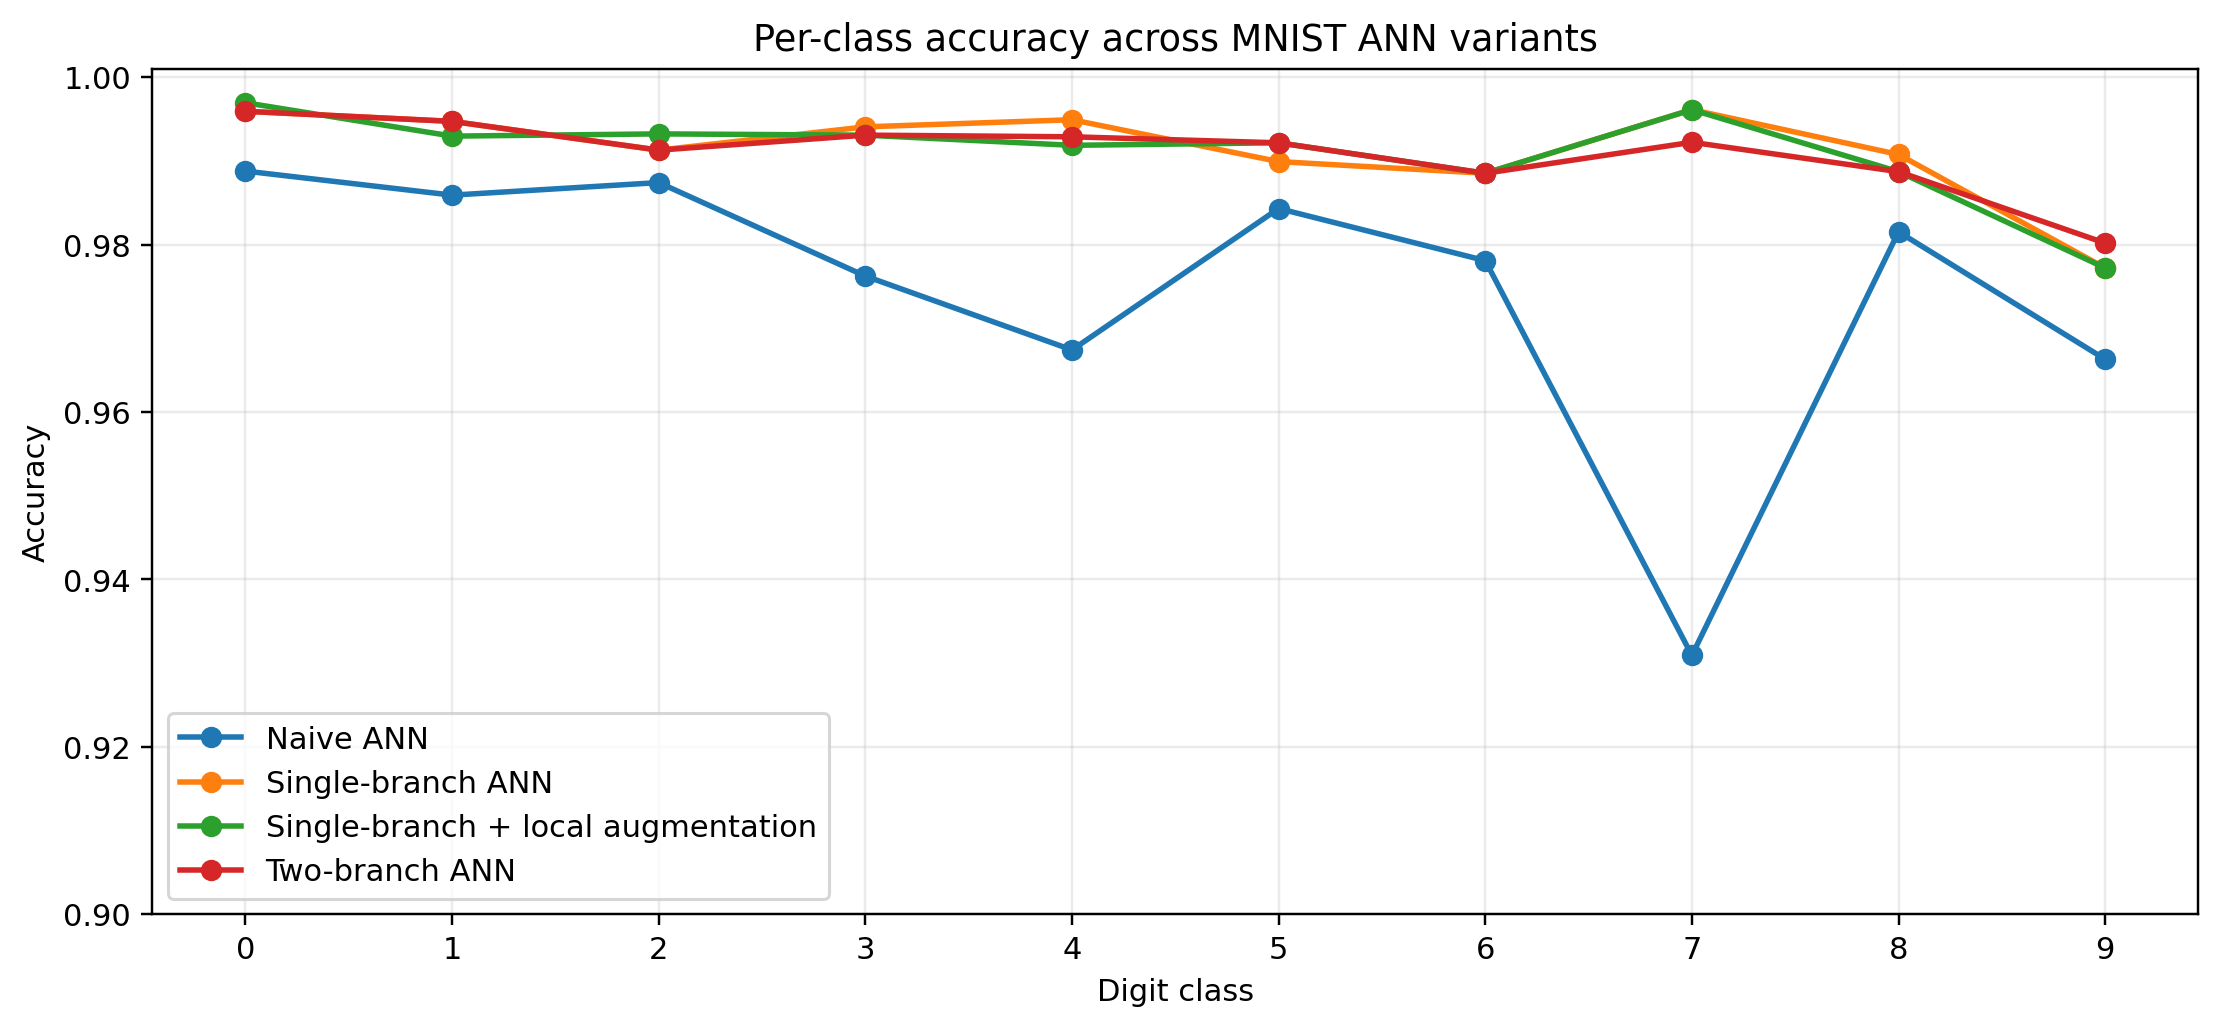
\includegraphics[width=0.92\textwidth]{figures/mnist-models/per_class_accuracy_comparison.png}
  \caption{So sánh accuracy theo từng lớp giữa bốn biến thể ANN trên MNIST.}
  \label{fig:mnist-per-class-comparison}
\end{figure}

Bảng so sánh tổng thể và biểu đồ tổng hợp cho thấy bức tranh rất rõ. Naive ANN là mốc khởi đầu hợp lý nhưng có \textit{generalization gap} lớn nhất và nhạy với biến thiên hình học. Việc thêm \textit{deslant + recenter + HOG + BatchNorm + Dropout} giúp mô hình nhảy vọt từ $97.46\%$ lên $99.14\%$, đồng thời kéo \textit{generalization gap} giảm hơn một nửa. Đây là cải tiến quan trọng nhất, xác nhận rằng phần lớn lợi ích đến từ việc biểu diễn dữ liệu đúng hơn chứ không phải chỉ làm mạng sâu hơn.

Biểu đồ accuracy theo từng lớp cho thấy sau khi thêm tiền xử lý và HOG, độ chính xác tăng gần như đồng đều trên toàn bộ 10 lớp, nhưng các lớp khó nhất vẫn là $9$, $6$ và $8$. Điều này cũng giải thích vì sao augmentation cục bộ chỉ mang lại chênh lệch rất nhỏ: MNIST vốn là bộ dữ liệu tương đối sạch, chữ số khá thẳng và biến thiên hình học toàn cục đã được xử lý phần lớn bởi \textit{deslant + recenter}. Vì vậy, sau khi đã chuẩn hóa hình học và thêm HOG, việc tiếp tục bơm \textit{elastic distortion} hay \textit{stroke jitter} không còn tạo ra thêm nhiều thông tin hữu ích cho mô hình.

Kết luận cho Chương 1 có thể chốt gọn bằng ba ý. Thứ nhất, cấu hình tốt nhất theo test accuracy trong loạt thử nghiệm hiện tại là \textit{Single-branch ANN} với $99.14\%$, nên trên MNIST lợi ích lớn nhất thật sự đến từ \textit{deslant + recenter + HOG} chứ không phải từ việc làm kiến trúc ngày càng phức tạp. Thứ hai, augmentation cục bộ không còn cần thiết sau khi dữ liệu đã được chuẩn hóa hình học; kết quả $99.11\%$ của biến thể có \textit{elastic distortion + stroke jitter} gần như không cải thiện gì so với single-branch gốc. Thứ ba, việc tách raw pixel và HOG thành hai nhánh riêng cũng không mang lại lợi ích thực nghiệm rõ rệt; two-branch ANN chỉ đạt $99.10\%$, thấp hơn nhẹ so với single-branch, cho thấy trong bối cảnh MNIST thì hợp nhất sớm raw pixel và HOG đã là lựa chọn đủ tốt. Vì vậy, insight quan trọng nhất của chương này là: với một bộ dữ liệu sạch như MNIST, ANN thuần vẫn rất hiệu quả nếu được cung cấp đúng biểu diễn đầu vào, còn các cải tiến phức tạp hơn chưa chắc tạo thêm lợi ích đáng kể.

\chapter{Phân loại FashionMNIST bằng ANN}

\section{Tổng quan}

Sau khi hoàn tất chuỗi thí nghiệm trên MNIST Handwritten, các mô hình ANN được chuyển sang FashionMNIST để kiểm tra khả năng tổng quát hóa trên một bộ dữ liệu khó hơn~\cite{xiao2017fashion,fashionmnist_repo}. Nếu MNIST chủ yếu khác nhau ở hướng nét và bố cục stroke, thì FashionMNIST khó hơn ở chỗ nhiều lớp có silhouette gần nhau, đặc biệt giữa \textit{T-shirt/top}, \textit{Shirt}, \textit{Pullover} và \textit{Coat}. Vì vậy, chương này cũng giữ đúng tinh thần của Chương 1: bắt đầu từ baseline naive chỉ dùng raw pixel, sau đó tăng dần mức độ đặc trưng hóa và độ ổn định dự đoán để xem yếu tố nào thực sự có ích trên dữ liệu thời trang.

\section{Phát biểu bài toán}

Bài toán cần giải quyết là phân lớp ảnh thời trang thành $10$ lớp như \textit{T-shirt/top}, \textit{Trouser}, \textit{Pullover}, \textit{Dress}, \textit{Coat}, \textit{Sandal}, \textit{Shirt}, \textit{Sneaker}, \textit{Bag} và \textit{Ankle boot}. Đầu vào của mô hình là ảnh xám kích thước $28 \times 28$, nên mỗi mẫu gốc có $784$ pixel. Đầu ra vẫn là vector logits $10$ chiều; lớp có logit lớn nhất được chọn làm nhãn dự đoán cuối cùng.

Về mặt dữ liệu, FashionMNIST cũng là bài toán \textit{single-label classification}. Trong Lab 03, dữ liệu được dùng theo đúng hai split chính thức của bộ dữ liệu: $60{,}000$ mẫu train để huấn luyện và $10{,}000$ mẫu test để đánh giá cuối~\cite{xiao2017fashion}. Không có validation riêng được tách ra, nên toàn bộ so sánh giữa các mô hình trong chương này đều bám trên cùng một protocol train/test.

\begin{table}[H]
\centering
\caption{Phát biểu bài toán và thiết lập dữ liệu của FashionMNIST}
\label{tab:fashion-mnist-problem-setup}
\begin{tabular}{l c}
\toprule
Thành phần & Giá trị \\
\midrule
Kiểu bài toán & Single-label classification \\
Đầu vào & Ảnh xám $28 \times 28$ \\
Đầu ra & Vector logits $10$ chiều \\
Số lớp & $10$ lớp thời trang \\
Train chính thức & $60{,}000$ mẫu \\
Test chính thức & $10{,}000$ mẫu \\
Thiết lập Lab 03 & Dùng toàn bộ train để huấn luyện, test ở cuối \\
\bottomrule
\end{tabular}
\end{table}


\section{Mô hình và tham số}
\subsection{Naive ANN}

Naive ANN là baseline tối giản nhất của chương này và cũng là điểm xuất phát cần thiết để kiểm tra xem ANN thuần có thể đi được đến đâu nếu chỉ nhìn ảnh thời trang ở mức pixel thô. Đầu vào của mô hình chỉ gồm raw pixel được trải phẳng thành vector $784$ chiều, hoàn toàn không có \textit{deslant}, \textit{recenter}, HOG hay bất kỳ augmentation nào. Lớp vào vì thế có đúng $784$ neuron, tương ứng trực tiếp với $784$ pixel của ảnh xám $28 \times 28$. Đầu ra là vector logits $10$ chiều để biểu diễn mười lớp trang phục; lớp có logit lớn nhất được chọn làm dự đoán cuối cùng.

Kiến trúc MLP được giữ cùng khuôn với baseline ở Chương 1:
\[
784 \rightarrow 1024 \rightarrow 512 \rightarrow 256 \rightarrow 10.
\]
Ba tầng ẩn dùng ReLU, còn hàm mất mát là \textit{cross-entropy} tiêu chuẩn. Cách chọn số chiều ẩn cũng mang cùng triết lý như ở MNIST: tầng đầu mở rộng lên $1024$ để mô hình có đủ không gian kết hợp các pixel thô thành những biểu diễn giàu hơn; hai tầng sau giảm dần về $512$ rồi $256$ để nén dần biểu diễn trước khi đi tới lớp phân loại. Việc không tiếp tục làm các tầng sau ngày càng rộng hơn giúp baseline tránh tăng quá mạnh số tham số trong khi đầu vào vẫn còn rất thô và thiếu cấu trúc. Optimizer được chọn là Adam để baseline hội tụ ổn định mà không thêm các kỹ thuật regularization phụ. Mục tiêu của biến thể này là trả lời trực tiếp câu hỏi: nếu chỉ dùng pixel thô, ANN có thể đi được tới đâu trên FashionMNIST.

\begin{table}[H]
\centering
\caption{Kết quả của naive ANN trên FashionMNIST}
\label{tab:fashion-mnist-naive-results}
\begin{tabular}{l c}
\toprule
Chỉ số & Giá trị \\
\midrule
Final train accuracy & 0.9796 \\
Test accuracy & 0.8959 \\
Generalization gap & 0.0837 \\
\bottomrule
\end{tabular}
\end{table}


\begin{figure}[H]
  \centering
  
\includegraphics[width=0.95\textwidth]{figures/fashion-mnist-naive/training_curves.png}
  \caption{Diễn biến train accuracy và train loss của naive ANN trên FashionMNIST trong 50 epoch.}
  \label{fig:fashion-mnist-naive-training-curves}
\end{figure}

\begin{figure}[H]
  \centering
  
\includegraphics[width=0.82\textwidth]{figures/fashion-mnist-naive/confusion_matrix.png}
  \caption{Confusion matrix của naive ANN trên FashionMNIST.}
  \label{fig:fashion-mnist-naive-confusion}
\end{figure}

\begin{figure}[H]
  \centering
  
\includegraphics[width=0.95\textwidth]{figures/fashion-mnist-naive/class_accuracy_bar.png}
  \caption{Accuracy theo từng lớp của naive ANN trên FashionMNIST.}
  \label{fig:fashion-mnist-naive-class-accuracy}
\end{figure}

\begin{table}[H]
\centering
\caption{Các cặp nhầm lẫn lớn nhất của naive ANN trên FashionMNIST}
\label{tab:fashion-mnist-naive-top-errors}
\begin{tabular}{l c}
\toprule
Cặp nhầm lẫn & Số mẫu \\
\midrule
T-shirt/top $\rightarrow$ Shirt & 125 \\
Shirt $\rightarrow$ T-shirt/top & 103 \\
Coat $\rightarrow$ Pullover & 101 \\
Pullover $\rightarrow$ Shirt & 79 \\
Coat $\rightarrow$ Shirt & 79 \\
Shirt $\rightarrow$ Pullover & 72 \\
Pullover $\rightarrow$ Coat & 56 \\
Ankle boot $\rightarrow$ Sneaker & 46 \\
\bottomrule
\end{tabular}
\end{table}


Naive ANN đạt $89.59\%$ test accuracy. Các cặp nhầm lẫn lớn nhất đã lộ ra rất rõ ngay từ baseline: \textit{T-shirt/top} $\rightarrow$ \textit{Shirt}, \textit{Shirt} $\rightarrow$ \textit{T-shirt/top}, \textit{Coat} $\rightarrow$ \textit{Pullover}, \textit{Pullover} $\rightarrow$ \textit{Shirt}. Điều này cho thấy với FashionMNIST, raw pixel đơn thuần chưa đủ để tách các lớp có hình dáng gần nhau, nhất là khi khác biệt nằm ở hướng biên, nếp áo và phân bố hình học tổng thể.

Từ kết quả này, bước tiếp theo hợp lý là thêm chuẩn hóa hình học và đặc trưng gradient để mô hình không chỉ nhìn cường độ pixel thô, mà còn nắm rõ hướng nét và cấu trúc biên của từng loại trang phục.

\subsection{Single-branch ANN}

Single-branch ANN là biến thể cải tiến trực tiếp từ baseline naive. Điểm xuất phát của biến thể này là insight vừa rút ra: raw pixel thuần chưa đủ để tách các lớp quần áo có silhouette gần nhau, nên mô hình cần được bổ sung thông tin hình học và hướng biên ngay từ đầu. Vì vậy, ảnh trước hết được chuẩn hóa bằng \textit{deslant + recenter} để làm ổn định bố cục tổng thể, sau đó biểu diễn đầu vào được mở rộng thành vector $2080 = 784 + 1296$ chiều, trong đó $784$ chiều đến từ raw pixel sau tiền xử lý và $1296$ chiều đến từ HOG. MLP phía sau có dạng:
\[
2080 \rightarrow 1024 \rightarrow 512 \rightarrow 256 \rightarrow 10.
\]
Ba tầng ẩn dùng BatchNorm, GELU và Dropout$(0.25)$. Kích thước $1024 \rightarrow 512 \rightarrow 256$ được giữ nguyên từ Chương 1 vì mục tiêu ở đây là kiểm tra khả năng chuyển giao của cấu hình mạnh nhất trên MNIST sang dữ liệu thời trang, thay vì thay đổi quá nhiều thành phần cùng lúc. Tầng đầu giữ ở mức $1024$ để hấp thụ đầu vào $2080$ chiều sau khi ghép raw pixel và HOG; các tầng sau tiếp tục giảm dần để nén biểu diễn và giữ cho phần phân loại cuối đủ gọn. BatchNorm được dùng để ổn định kích hoạt khi đầu vào đã là sự kết hợp của hai nguồn đặc trưng khác bản chất, còn Dropout được thêm để giảm độ nhạy của các lớp fully-connected tương đối rộng. Loss tiếp tục là \textit{cross-entropy} có \textit{label smoothing} $0.05$, còn optimizer là AdamW với cosine scheduler nhằm giữ quá trình tối ưu ổn định hơn so với baseline.

\begin{table}[H]
\centering
\caption{Kết quả single-branch ANN trên FashionMNIST}
\label{tab:fashion-mnist-single-branch-results}
\begin{tabular}{l c}
\toprule
Chỉ số & Giá trị \\
\midrule
Final train accuracy & 0.99997 \\
Final train loss & 0.2906 \\
Test accuracy & 0.9060 \\
Generalization gap & 0.0940 \\
Epochs & 50 \\
\bottomrule
\end{tabular}
\end{table}


\begin{figure}[H]
  \centering
  
\includegraphics[width=0.95\textwidth]{figures/fashion-mnist-ann/training_curves.png}
  \caption{Diễn biến train accuracy và train loss của single-branch ANN trên FashionMNIST trong 50 epoch.}
  \label{fig:fashion-mnist-training-curves}
\end{figure}

\begin{figure}[H]
  \centering
  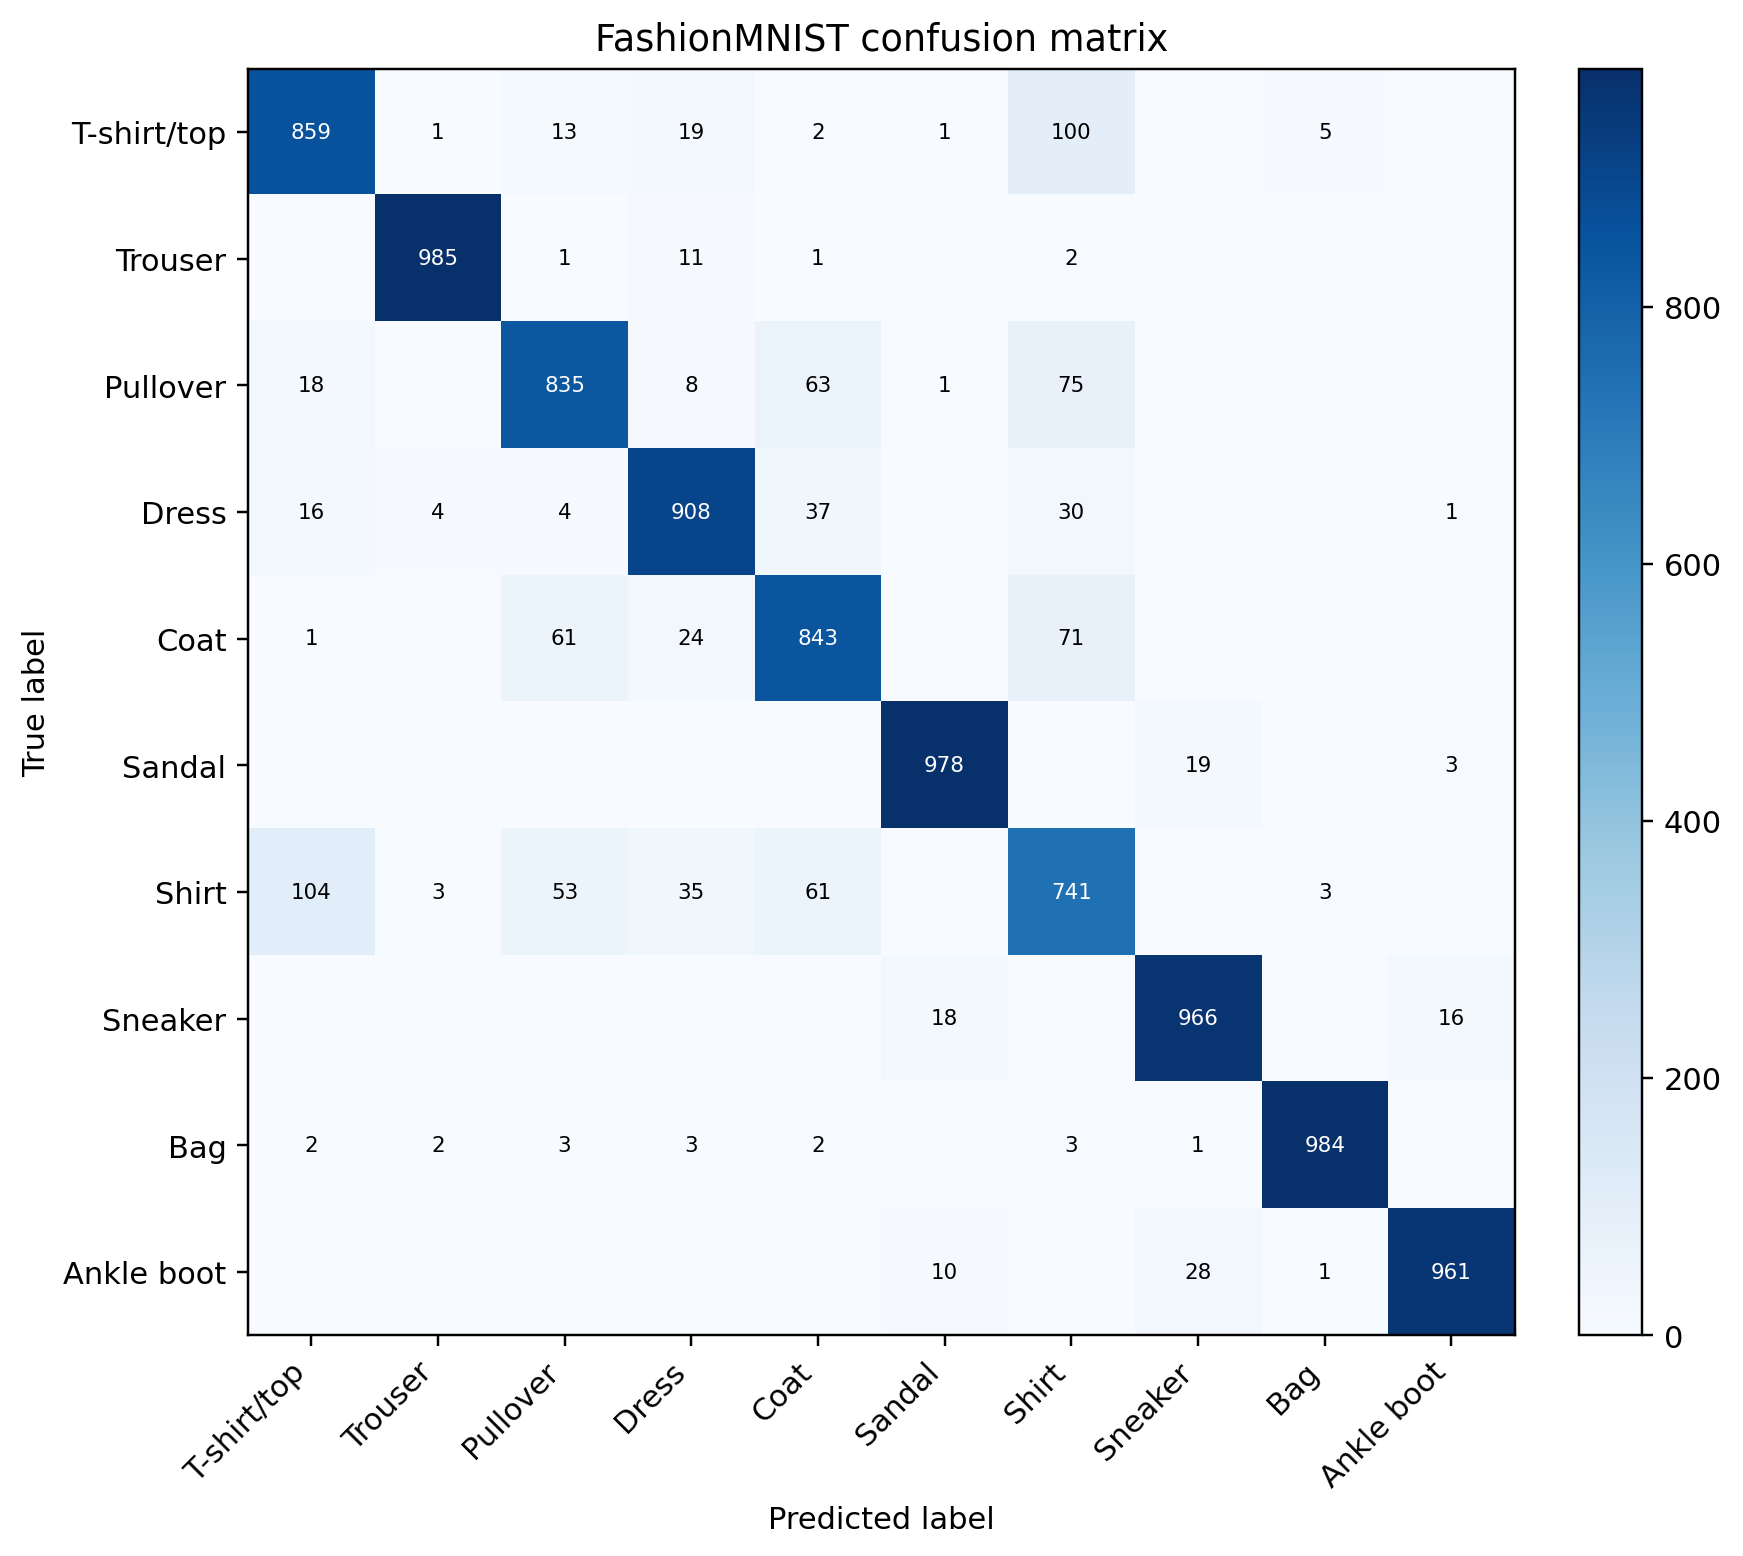
\includegraphics[width=0.82\textwidth]{figures/fashion-mnist-ann/confusion_matrix.png}
  \caption{Confusion matrix của single-branch ANN trên FashionMNIST.}
  \label{fig:fashion-mnist-confusion}
\end{figure}

\begin{figure}[H]
  \centering
  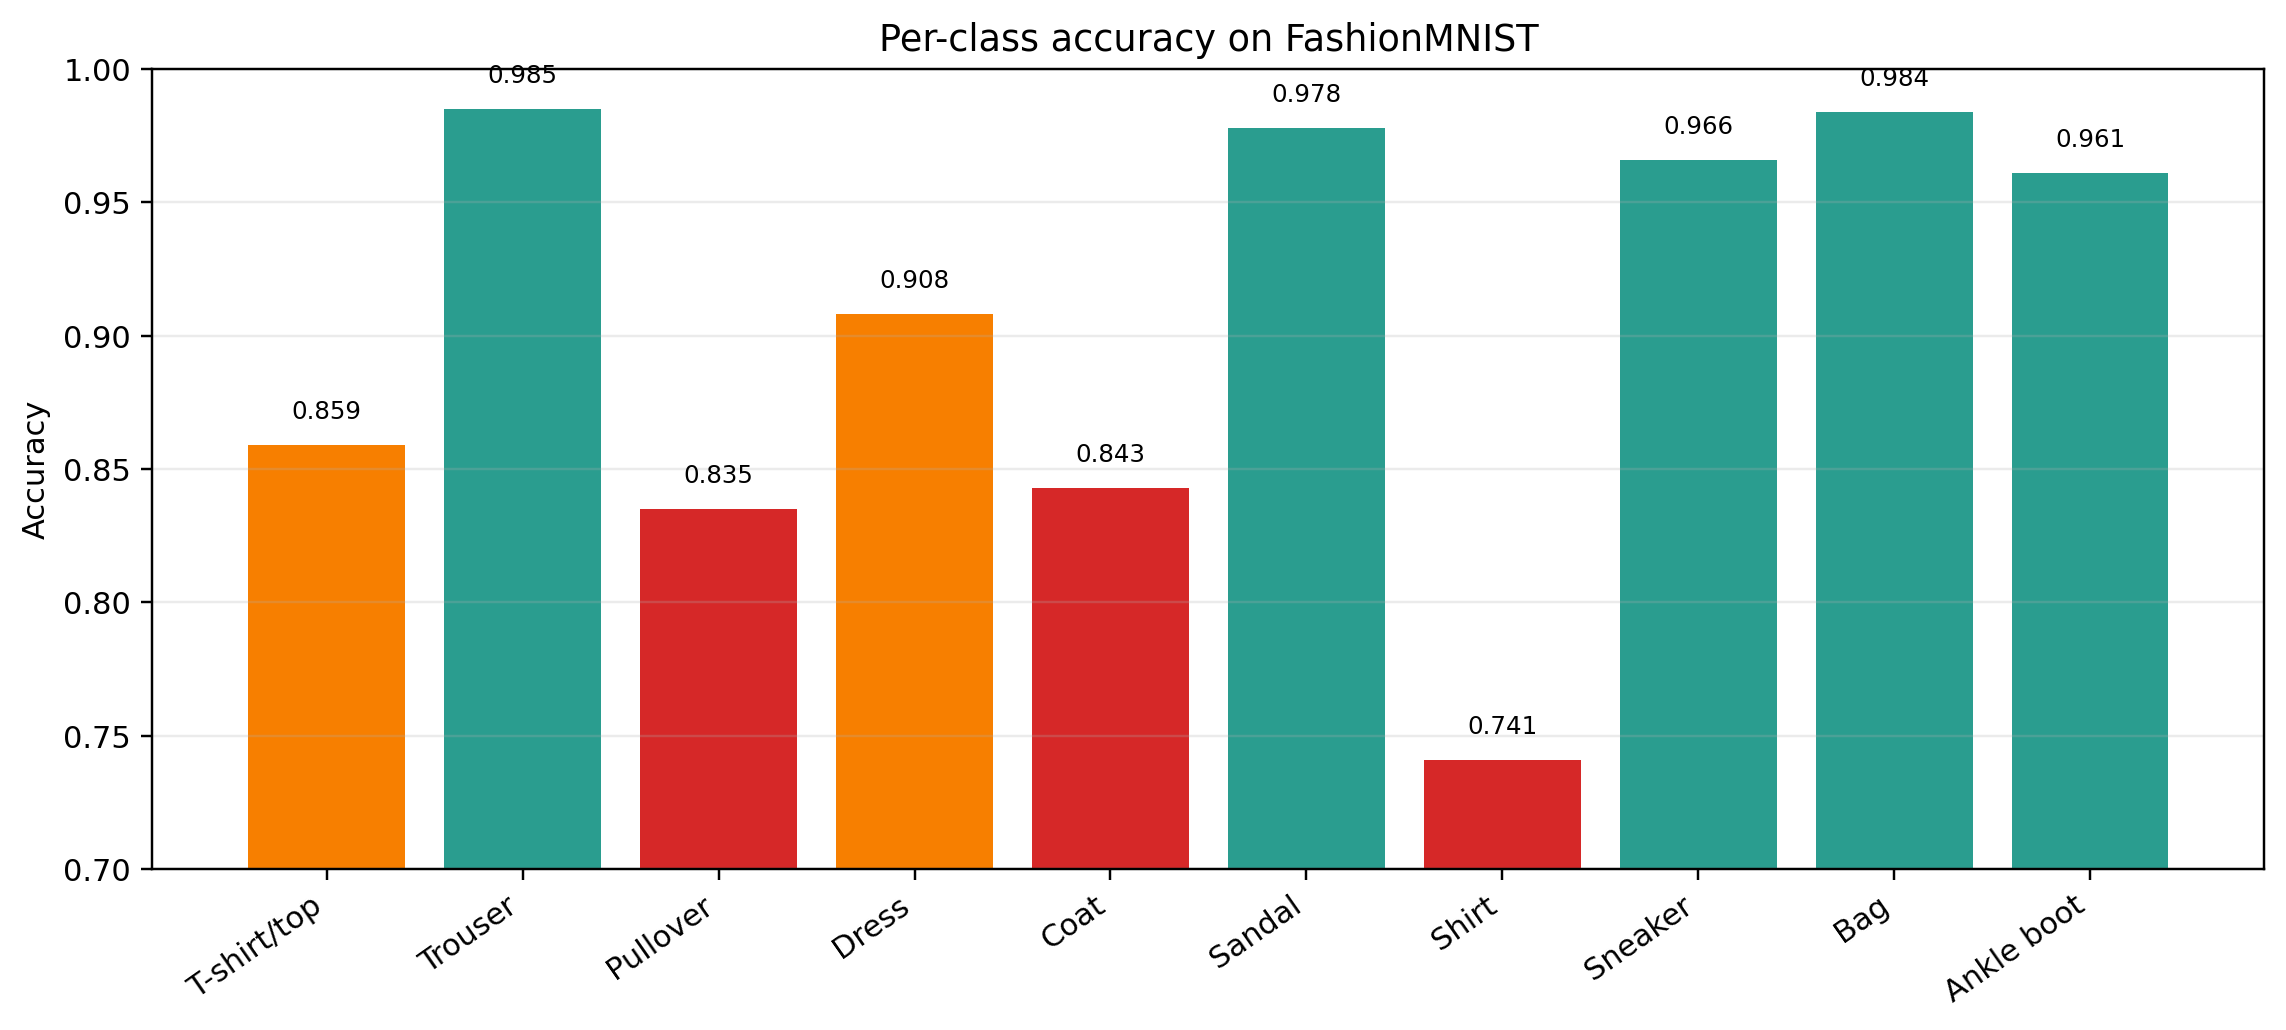
\includegraphics[width=0.95\textwidth]{figures/fashion-mnist-ann/class_accuracy_bar.png}
  \caption{Accuracy theo từng lớp của single-branch ANN trên FashionMNIST.}
  \label{fig:fashion-mnist-class-accuracy}
\end{figure}

\begin{table}[H]
\centering
\caption{Các cặp nhầm lẫn lớn nhất của single-branch ANN trên FashionMNIST}
\label{tab:fashion-mnist-top-errors}
\begin{tabular}{l c}
\toprule
Cặp nhầm lẫn & Số mẫu \\
\midrule
Shirt $\rightarrow$ T-shirt/top & 104 \\
T-shirt/top $\rightarrow$ Shirt & 100 \\
Pullover $\rightarrow$ Shirt & 75 \\
Coat $\rightarrow$ Shirt & 71 \\
Pullover $\rightarrow$ Coat & 63 \\
Shirt $\rightarrow$ Coat & 61 \\
Coat $\rightarrow$ Pullover & 61 \\
Shirt $\rightarrow$ Pullover & 53 \\
\bottomrule
\end{tabular}
\end{table}


Single-branch ANN đạt \textit{test accuracy} $90.60\%$ với \textit{generalization gap} khoảng $9.4\%$, thấp hơn đáng kể so với mức hơn $99\%$ trên MNIST. Confusion matrix và bảng top lỗi cho thấy khó khăn tập trung mạnh vào các lớp áo có hình dáng gần nhau, nổi bật nhất là \textit{Shirt} $\rightarrow$ \textit{T-shirt/top}, \textit{T-shirt/top} $\rightarrow$ \textit{Shirt}, \textit{Pullover} $\rightarrow$ \textit{Shirt} và \textit{Coat} $\rightarrow$ \textit{Shirt}. Điều này cho thấy với FashionMNIST, đặc trưng hình học cơ bản đã giúp nhiều nhưng vẫn chưa đủ để tách các lớp chồng lấn mạnh về silhouette.

Từ kết quả này, giả thuyết kế tiếp là: nếu raw pixel và HOG đang bị hòa trộn quá sớm ở đầu vào chung, có thể việc tách chúng thành hai nhánh riêng sẽ giúp mỗi nguồn đặc trưng học vai trò chuyên biệt hơn trước khi hợp nhất.

\subsection{Two-branch ANN}

Two-branch ANN dùng cùng đầu vào và cùng pipeline \textit{deslant + recenter + HOG} như single-branch, nhưng thay vì ghép raw pixel và HOG ngay từ đầu, mô hình tách chúng thành hai nhánh riêng. Insight dẫn tới biến thể này là: nếu raw pixel và HOG có vai trò khác nhau, việc ép chúng đi qua cùng một tầng đầu có thể làm thông tin bị hòa trộn quá sớm. Vì vậy, nhánh raw có dạng $784 \rightarrow 512 \rightarrow 256$, nhánh HOG có dạng $1296 \rightarrow 768 \rightarrow 256$, sau đó hai vector $256$ chiều được ghép lại thành $512$ chiều và đi qua head cuối:
\[
512 \rightarrow 256 \rightarrow 10.
\]
Ý tưởng của biến thể này hoàn toàn giống Chương 1: raw pixel và HOG có bản chất khác nhau, nên có thể có lợi nếu cho chúng học biểu diễn riêng trước khi hợp nhất. Nhánh HOG được cấp tầng đầu rộng hơn vì đầu vào của nó nhiều chiều hơn và mang sẵn thông tin cấu trúc mạnh hơn raw pixel; cả hai nhánh đều được nén về $256$ chiều để quá trình hợp nhất ở phần head không bị lệch hẳn về một bên.

\begin{table}[H]
\centering
\caption{Kết quả two-branch ANN trên FashionMNIST}
\label{tab:fashion-mnist-two-branch-results}
\begin{tabular}{l c}
\toprule
Chỉ số & Giá trị \\
\midrule
Final train accuracy & 0.99987 \\
Final train loss & 0.2918 \\
Test accuracy & 0.8969 \\
Generalization gap & 0.1030 \\
Epochs & 50 \\
\bottomrule
\end{tabular}
\end{table}


\begin{figure}[H]
  \centering
  
\includegraphics[width=0.95\textwidth]{figures/fashion-mnist-two-branch/training_curves.png}
  \caption{Diễn biến train accuracy và train loss của two-branch ANN trên FashionMNIST trong 50 epoch.}
  \label{fig:fashion-mnist-two-branch-training-curves}
\end{figure}

\begin{figure}[H]
  \centering
  
\includegraphics[width=0.82\textwidth]{figures/fashion-mnist-two-branch/confusion_matrix.png}
  \caption{Confusion matrix của two-branch ANN trên FashionMNIST.}
  \label{fig:fashion-mnist-two-branch-confusion}
\end{figure}

\begin{figure}[H]
  \centering
  
\includegraphics[width=0.95\textwidth]{figures/fashion-mnist-two-branch/class_accuracy_bar.png}
  \caption{Accuracy theo từng lớp của two-branch ANN trên FashionMNIST.}
  \label{fig:fashion-mnist-two-branch-class-accuracy}
\end{figure}

\begin{table}[H]
\centering
\caption{Các cặp nhầm lẫn lớn nhất của two-branch ANN trên FashionMNIST}
\label{tab:fashion-mnist-two-branch-top-errors}
\begin{tabular}{l c}
\toprule
Cặp nhầm lẫn & Số mẫu \\
\midrule
T-shirt/top $\rightarrow$ Shirt & 120 \\
Shirt $\rightarrow$ T-shirt/top & 102 \\
Pullover $\rightarrow$ Shirt & 87 \\
Coat $\rightarrow$ Shirt & 80 \\
Coat $\rightarrow$ Pullover & 70 \\
Shirt $\rightarrow$ Coat & 62 \\
Shirt $\rightarrow$ Pullover & 57 \\
Pullover $\rightarrow$ Coat & 49 \\
\bottomrule
\end{tabular}
\end{table}


Two-branch ANN chỉ đạt $89.69\%$ test accuracy và có \textit{generalization gap} khoảng $10.3\%$, tức còn thấp hơn single-branch. Mẫu lỗi vẫn gần như giữ nguyên: \textit{T-shirt/top} $\leftrightarrow$ \textit{Shirt}, \textit{Pullover} $\rightarrow$ \textit{Shirt}, \textit{Coat} $\rightarrow$ \textit{Shirt}. Điều này cho thấy trên FashionMNIST, bottleneck không còn nằm ở chỗ raw pixel và HOG có bị ghép quá sớm hay không; khó khăn chính là ranh giới lớp chồng lấn mạnh, và việc tăng độ phức tạp của kiến trúc chưa đủ để giải quyết.

Từ đây, hướng đi hợp lý hơn là không cố làm kiến trúc phức tạp hơn nữa, mà giữ biến thể đơn tốt nhất rồi giảm phương sai dự đoán bằng ensemble nhiều seed.

\subsection{Ensemble các mô hình single-branch}

Sau khi two-branch không cải thiện, bước tiếp theo không còn là làm kiến trúc phức tạp hơn, mà là kiểm tra xem single-branch có đang bị giới hạn bởi phương sai do khởi tạo và thứ tự mini-batch hay không. Vì vậy, biến thể này giữ nguyên toàn bộ cấu hình single-branch tốt nhất của chương: cùng đầu vào $2080 = 784 + 1296$, cùng kiến trúc
\[
2080 \rightarrow 1024 \rightarrow 512 \rightarrow 256 \rightarrow 10,
\]
cùng BatchNorm, GELU, Dropout$(0.25)$, AdamW, cross-entropy với label smoothing và cosine scheduler. Mô hình được huấn luyện độc lập ba lần với seed $42$, $52$ và $62$.

Động lực học của lựa chọn này khá trực tiếp: nếu mỗi mô hình đơn đã học được đặc trưng tương đối tốt nhưng nghiệm tối ưu cuối cùng còn nhạy với seed, thì việc lấy trung bình xác suất softmax ở bước test sẽ giúp làm phẳng dao động giữa các nghiệm đó. Nói cách khác, ensemble ở đây không nhằm thay đổi biểu diễn đầu vào, mà nhằm giảm phương sai dự đoán trong khi vẫn giữ nguyên biến thể đơn tốt nhất để so sánh công bằng.

\begin{table}[H]
\centering
\caption{Ba mô hình thành phần trong ensemble single-branch ANN trên FashionMNIST}
\label{tab:fashion-mnist-ensemble-member-details}
\small
\begin{tabularx}{\textwidth}{>{\raggedright\arraybackslash}p{2.2cm} >{\raggedright\arraybackslash}p{1.4cm} >{\raggedright\arraybackslash}p{3.2cm} >{\raggedright\arraybackslash}p{3.2cm} >{\raggedright\arraybackslash}X}
\toprule
Mô hình & Seed & Đầu vào & Kiến trúc & Huấn luyện \\
\midrule
Model 1 & 42 & $2080 = 784 + 1296$ & $2080 \rightarrow 1024 \rightarrow 512 \rightarrow 256 \rightarrow 10$ & AdamW, CE+LS, cosine, batch $256$, epoch $50$ \\
Model 2 & 52 & $2080 = 784 + 1296$ & $2080 \rightarrow 1024 \rightarrow 512 \rightarrow 256 \rightarrow 10$ & AdamW, CE+LS, cosine, batch $256$, epoch $50$ \\
Model 3 & 62 & $2080 = 784 + 1296$ & $2080 \rightarrow 1024 \rightarrow 512 \rightarrow 256 \rightarrow 10$ & AdamW, CE+LS, cosine, batch $256$, epoch $50$ \\
\bottomrule
\end{tabularx}
\end{table}

\begin{table}[H]
\centering
\caption{So sánh các seed single-branch ANN và ensemble trên FashionMNIST}
\label{tab:fashion-mnist-seed-comparison}
\begin{tabular}{l c c c}
\toprule
Cấu hình & Final train acc & Test acc & Generalization gap \\
\midrule
Seed 42 & 0.99992 & 0.9074 & 0.0925 \\
Seed 52 & 0.99995 & 0.9086 & 0.0914 \\
Seed 62 & 0.99992 & 0.9074 & 0.0925 \\
Ensemble (3 models) & -- & 0.9168 & -- \\
\bottomrule
\end{tabular}
\end{table}

\begin{table}[H]
\centering
\caption{Kết quả ensemble 3 mô hình single-branch ANN trên FashionMNIST}
\label{tab:fashion-mnist-ensemble-results}
\begin{tabular}{l c}
\toprule
Chỉ số & Giá trị \\
\midrule
Test accuracy & 0.9168 \\
Số mô hình trong ensemble & 3 \\
\bottomrule
\end{tabular}
\end{table}


\begin{figure}[H]
  \centering
  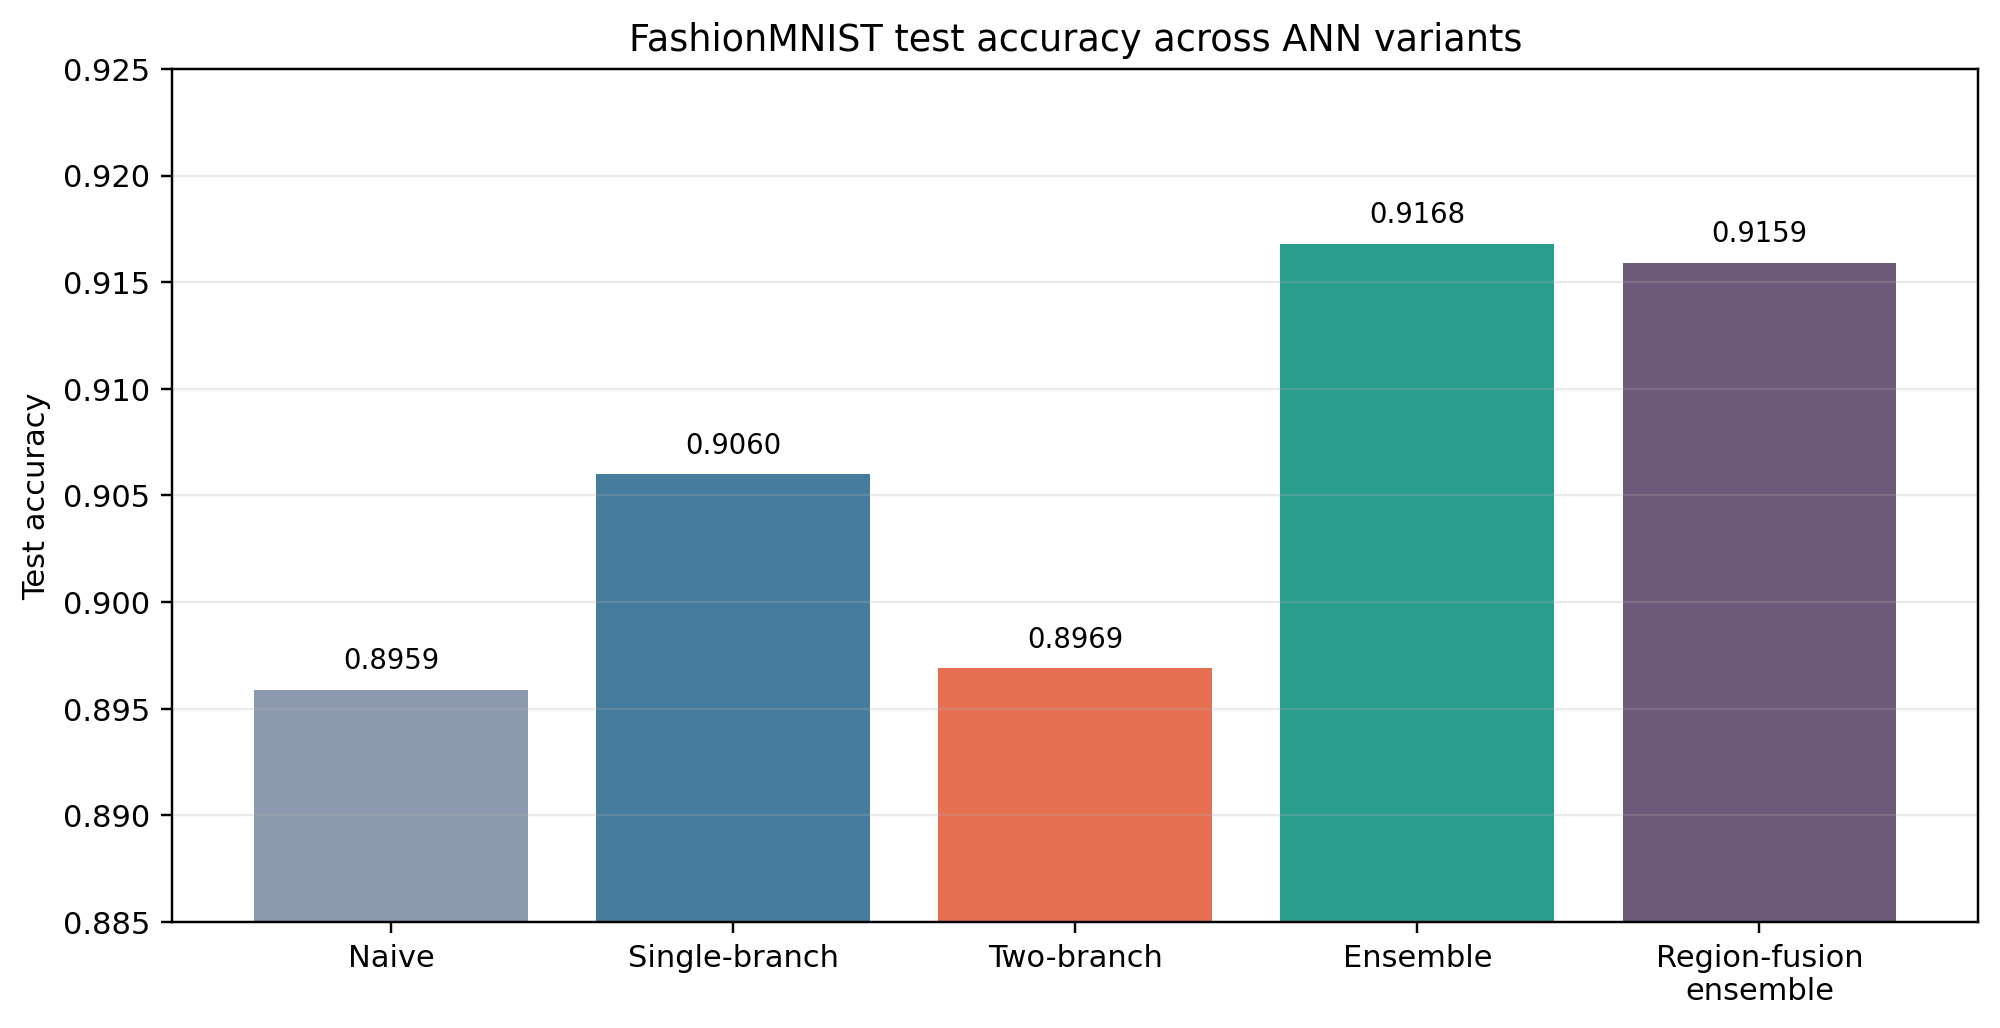
\includegraphics[width=0.95\textwidth]{figures/fashion-mnist-comparison/model_accuracy_comparison.png}
  \caption{So sánh test accuracy giữa các cấu hình ANN trên FashionMNIST.}
  \label{fig:fashion-mnist-model-comparison}
\end{figure}

\begin{figure}[H]
  \centering
  
\includegraphics[width=0.82\textwidth]{figures/fashion-mnist-ensemble/confusion_matrix.png}
  \caption{Confusion matrix của ensemble 3 mô hình single-branch ANN trên FashionMNIST.}
  \label{fig:fashion-mnist-ensemble-confusion}
\end{figure}

\begin{figure}[H]
  \centering
  
\includegraphics[width=0.95\textwidth]{figures/fashion-mnist-ensemble/class_accuracy_bar.png}
  \caption{Accuracy theo từng lớp của ensemble 3 mô hình single-branch ANN trên FashionMNIST.}
  \label{fig:fashion-mnist-ensemble-class-accuracy}
\end{figure}

\begin{table}[H]
\centering
\caption{Các cặp nhầm lẫn lớn nhất của ensemble single-branch ANN trên FashionMNIST}
\label{tab:fashion-mnist-ensemble-top-errors}
\begin{tabular}{l c}
\toprule
Cặp nhầm lẫn & Số mẫu \\
\midrule
T-shirt/top $\rightarrow$ Shirt & 95 \\
Shirt $\rightarrow$ T-shirt/top & 79 \\
Pullover $\rightarrow$ Shirt & 65 \\
Coat $\rightarrow$ Shirt & 63 \\
Shirt $\rightarrow$ Pullover & 59 \\
Shirt $\rightarrow$ Coat & 58 \\
Coat $\rightarrow$ Pullover & 50 \\
Pullover $\rightarrow$ Coat & 44 \\
\bottomrule
\end{tabular}
\end{table}


Ensemble đạt $91.68\%$ test accuracy, cao hơn tất cả các mô hình đơn trước đó. Các cặp nhầm lẫn khó nhất vẫn không biến mất, nhưng số lượng lỗi ở những cặp như \textit{T-shirt/top} $\rightarrow$ \textit{Shirt} hay \textit{Shirt} $\rightarrow$ \textit{T-shirt/top} đều giảm xuống. Điều này cho thấy trên FashionMNIST, vấn đề không phải là một mô hình đơn lẻ không đủ mạnh để học đặc trưng, mà là quyết định cuối còn nhạy với seed và nhiễu của từng lượt huấn luyện; ensemble giúp làm phẳng dao động đó. Nhìn theo benchmark công khai của bộ dữ liệu, đây cũng là hướng cải tiến tự nhiên khi MLP đơn đã chạm trần tương đối rõ~\cite{fashionmnist_repo}.

\subsection{Region-focused feature fusion + ensemble}

Từ kết quả của ensemble single-branch, điểm nghẽn còn lại vẫn tập trung gần như hoàn toàn ở nhóm lớp áo phần thân trên, đặc biệt là \textit{T-shirt/top}, \textit{Shirt}, \textit{Pullover} và \textit{Coat}. Insight rút ra ở đây là HOG toàn ảnh và raw pixel đã mô tả tốt silhouette tổng thể, nhưng chưa nhấn đủ mạnh những khác biệt cục bộ ở cổ áo, vai và độ xòe của tay áo. Vì vậy, biến thể tiếp theo vẫn giữ đúng khung single-branch ensemble để so sánh công bằng, nhưng thay đầu vào bằng bộ đặc trưng giàu thông tin vùng hơn:
\[
2814 = 784 + 1296 + 648 + 16 + 56 + 14,
\]
trong đó $784$ là raw pixel, $1296$ là HOG toàn ảnh, $648$ là HOG của nửa trên ảnh, $16$ là zoning density trên lưới $4 \times 4$, $56$ là row/column projection, và $14$ là upper-width profile. Mục tiêu của thiết kế này là làm cho mô hình nhìn rõ hơn phần thân trên của trang phục, thay vì chỉ dựa vào hình dáng tổng thể của toàn vật thể.

Kiến trúc của mỗi mô hình thành phần vẫn giữ đúng một form MLP đơn để việc so sánh chỉ còn phụ thuộc vào đầu vào:
\[
2814 \rightarrow 1024 \rightarrow 512 \rightarrow 256 \rightarrow 10,
\]
đi kèm BatchNorm, GELU, Dropout$(0.25)$, AdamW, cross-entropy với label smoothing và cosine scheduler. Việc cố ý không đổi phần thân mạng có ý nghĩa rất quan trọng: nếu kết quả thay đổi, có thể quy cải thiện hoặc suy giảm chủ yếu cho bộ đặc trưng vùng thân trên, thay vì do khác biệt về optimizer, regularization hay độ rộng mạng.

\begin{table}[H]
\centering
\caption{So sánh các seed của ensemble region-fusion trên FashionMNIST}
\label{tab:fashion-mnist-region-fusion-seed-comparison}
\begin{tabular}{l c c c}
\toprule
Cấu hình & Final train acc & Test acc & Generalization gap \\
\midrule
Seed 42 & 0.99998 & 0.9064 & 0.0936 \\
Seed 52 & 0.99990 & 0.9109 & 0.0890 \\
Seed 62 & 0.99993 & 0.9102 & 0.0897 \\
Ensemble (3 models) & -- & 0.9159 & -- \\
\bottomrule
\end{tabular}
\end{table}

\begin{table}[H]
\centering
\caption{Kết quả ensemble 3 mô hình ANN với đặc trưng vùng thân trên trên FashionMNIST}
\label{tab:fashion-mnist-region-fusion-results}
\begin{tabular}{l c}
\toprule
Chỉ số & Giá trị \\
\midrule
Test accuracy & 0.9159 \\
Số mô hình trong ensemble & 3 \\
Đầu vào mỗi mô hình & $2814 = 784 + 1296 + 648 + 16 + 56 + 14$ \\
\bottomrule
\end{tabular}
\end{table}


\begin{figure}[H]
  \centering
  
\includegraphics[width=0.82\textwidth]{figures/fashion-mnist-region-fusion/confusion_matrix.png}
  \caption{Confusion matrix của region-focused feature fusion ensemble trên FashionMNIST.}
  \label{fig:fashion-mnist-region-fusion-confusion}
\end{figure}

\begin{figure}[H]
  \centering
  
\includegraphics[width=0.95\textwidth]{figures/fashion-mnist-region-fusion/class_accuracy_bar.png}
  \caption{Accuracy theo từng lớp của region-focused feature fusion ensemble trên FashionMNIST.}
  \label{fig:fashion-mnist-region-fusion-class-accuracy}
\end{figure}

\begin{figure}[H]
  \centering
  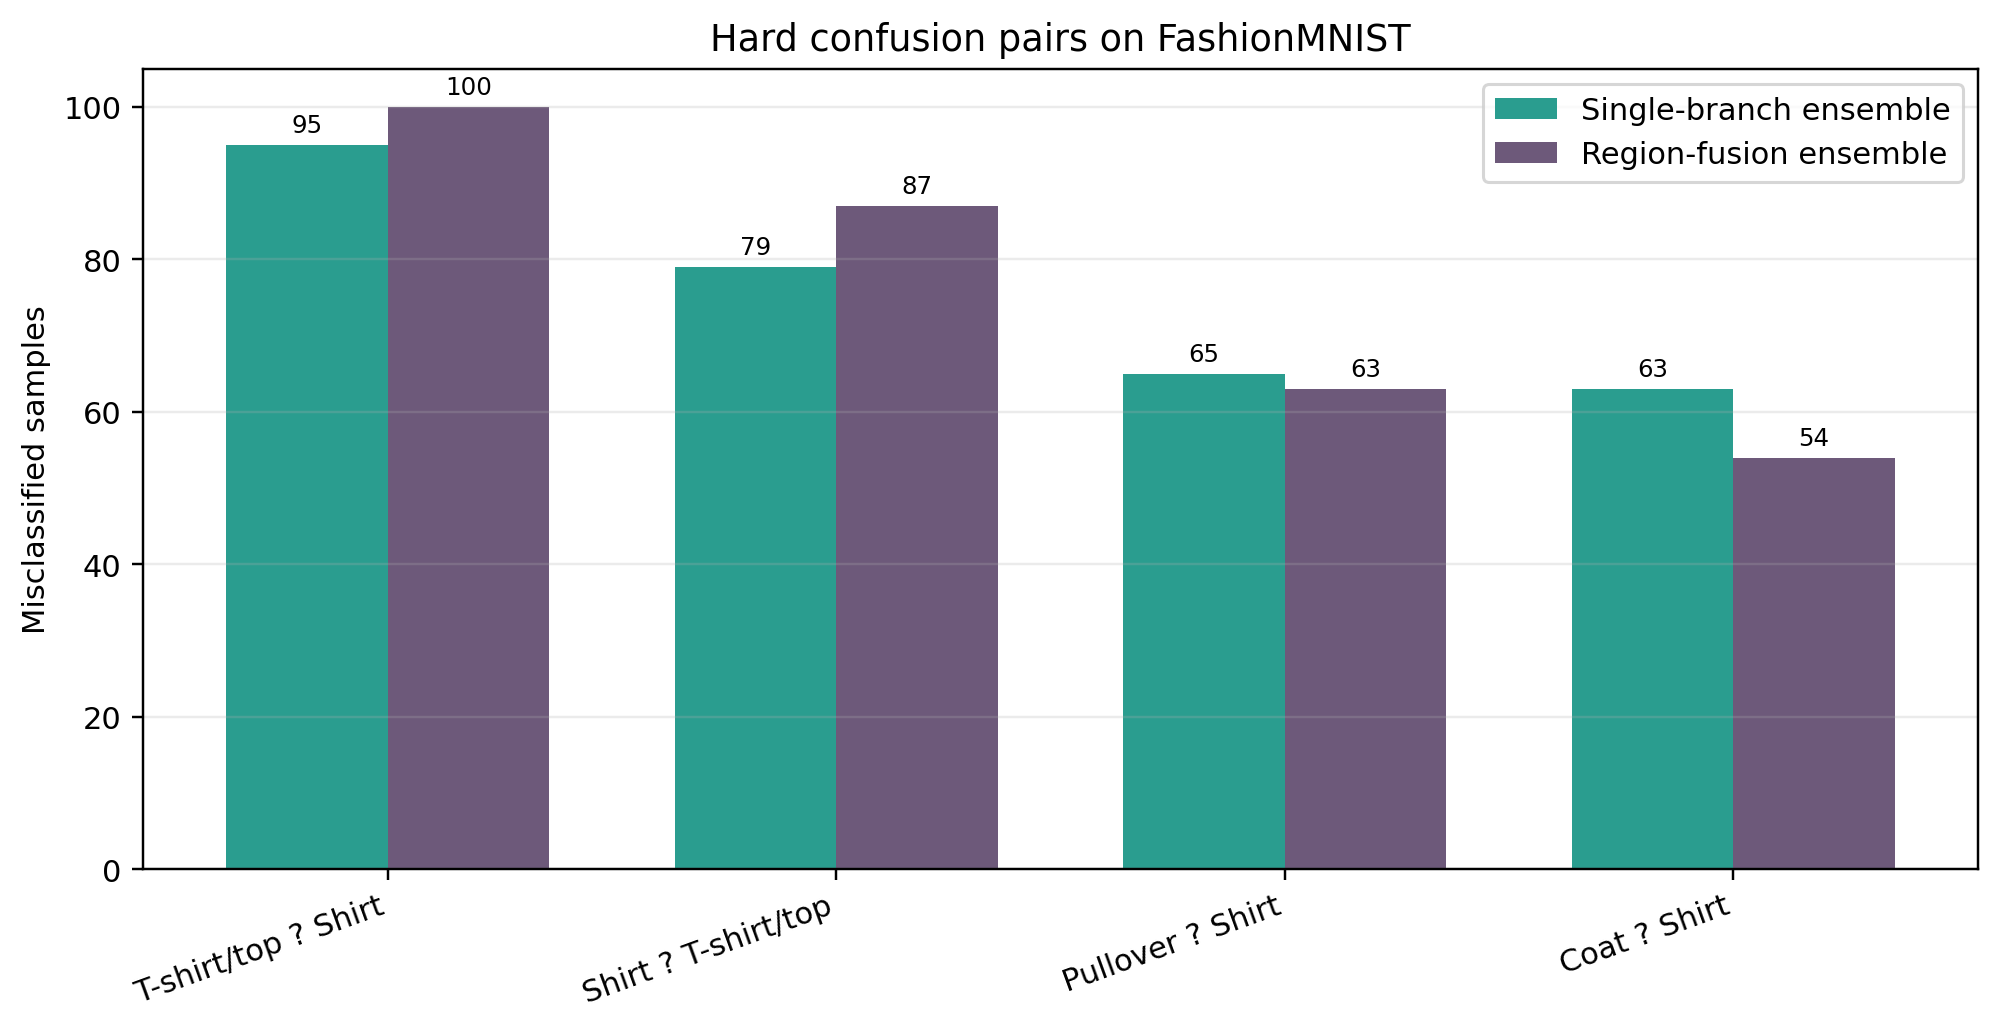
\includegraphics[width=0.92\textwidth]{figures/fashion-mnist-comparison/shirt_confusion_comparison.png}
  \caption{So sánh các cặp nhầm lẫn khó nhất giữa ensemble single-branch và region-focused feature fusion ensemble.}
  \label{fig:fashion-mnist-shirt-confusion-comparison}
\end{figure}

\begin{table}[H]
\centering
\caption{Các cặp nhầm lẫn lớn nhất của region-fusion ensemble trên FashionMNIST}
\label{tab:fashion-mnist-region-fusion-top-errors}
\begin{tabular}{l c}
\toprule
Cặp nhầm lẫn & Số mẫu \\
\midrule
T-shirt/top $\rightarrow$ Shirt & 100 \\
Shirt $\rightarrow$ T-shirt/top & 87 \\
Shirt $\rightarrow$ Coat & 68 \\
Pullover $\rightarrow$ Shirt & 63 \\
Pullover $\rightarrow$ Coat & 54 \\
Coat $\rightarrow$ Shirt & 54 \\
Coat $\rightarrow$ Pullover & 51 \\
Shirt $\rightarrow$ Pullover & 50 \\
\bottomrule
\end{tabular}
\end{table}


Kết quả thu được là $91.59\%$ test accuracy, tức rất sát nhưng vẫn thấp hơn nhẹ so với ensemble single-branch ($91.68\%$). Điều này cho thấy giả thuyết \textit{thêm đặc trưng tập trung vào vùng thân trên sẽ tiếp tục cải thiện kết quả} không được xác nhận trong bộ dữ liệu hiện tại. Thực tế, các cặp nhầm lẫn chính như \textit{T-shirt/top} $\rightarrow$ \textit{Shirt} và \textit{Shirt} $\rightarrow$ \textit{T-shirt/top} không giảm mà còn tăng nhẹ từ $95/79$ lên $100/87$. Nói cách khác, hướng feature engineering này có lý về mặt trực giác, nhưng ở độ phân giải $28 \times 28$ của FashionMNIST, phần thông tin hình học bổ sung ở nửa trên vẫn chưa đủ sạch để vượt qua ensemble single-branch gốc.

\section{Tổng hợp kết quả và nhận xét}

\begin{table}[H]
\centering
\caption{Kiến trúc các biến thể ANN trên FashionMNIST}
\label{tab:fashion-ann-architecture-details}
\small
\begin{tabularx}{\textwidth}{>{\raggedright\arraybackslash}p{3cm} >{\raggedright\arraybackslash}p{3.2cm} >{\raggedright\arraybackslash}X >{\raggedright\arraybackslash}p{3.1cm}}
\toprule
Biến thể & Đầu vào & Kiến trúc & Thành phần chính \\
\midrule
Naive ANN & Raw pixel $784$ & $784 \rightarrow 1024 \rightarrow 512 \rightarrow 256 \rightarrow 10$ & ReLU + fully-connected \\
Single-branch ANN & $2080 = 784 + 1296$ & $2080 \rightarrow 1024 \rightarrow 512 \rightarrow 256 \rightarrow 10$ & BN + GELU + Dropout$(0.25)$ \\
Two-branch ANN & Raw $784$, HOG $1296$ & Raw: $784 \rightarrow 512 \rightarrow 256$; HOG: $1296 \rightarrow 768 \rightarrow 256$; head: $512 \rightarrow 256 \rightarrow 10$ & BN + GELU + Dropout$(0.25)$ \\
Single-branch ensemble & 3 mô hình single-branch độc lập & Trung bình softmax probability của ba seed $42/52/62$ & Ensemble xác suất \\
Region-fusion ensemble & $2814 = 784 + 1296 + 648 + 16 + 56 + 14$ & 3 mô hình $2814 \rightarrow 1024 \rightarrow 512 \rightarrow 256 \rightarrow 10$ & HOG vùng trên + zoning + projection + ensemble \\
\bottomrule
\end{tabularx}
\end{table}

\begin{table}[H]
\centering
\caption{Thông số huấn luyện của các biến thể ANN trên FashionMNIST}
\label{tab:fashion-ann-hyperparameters}
\small
\begin{tabularx}{\textwidth}{>{\raggedright\arraybackslash}p{3cm} >{\raggedright\arraybackslash}p{3.2cm} >{\raggedright\arraybackslash}p{2.2cm} >{\raggedright\arraybackslash}X}
\toprule
Biến thể & Tối ưu hóa & Batch/epoch & Tiền xử lý và augmentation \\
\midrule
Naive ANN & Adam, CE, không scheduler & $256 / 50$ & Chỉ raw pixel, không tiền xử lý bổ sung \\
Single-branch ANN & AdamW, CE+LS, cosine, $wd=10^{-4}$ & $256 / 50$ & Affine; deslant; recenter; HOG \\
Two-branch ANN & AdamW, CE+LS, cosine, $wd=10^{-4}$ & $256 / 50$ & Affine; deslant; recenter; tách raw/HOG \\
Single-branch ensemble & 3 lần chạy single-branch với seed khác nhau & $256 / 50$ mỗi mô hình & Cùng pipeline single-branch; ensemble ở bước test \\
Region-fusion ensemble & 3 lần chạy ANN vùng thân trên với seed khác nhau & $256 / 50$ mỗi mô hình & HOG toàn ảnh + HOG nửa trên + zoning + projection; ensemble ở bước test \\
\bottomrule
\end{tabularx}
\end{table}

\begin{table}[H]
\centering
\caption{Logic chuyển từ một biến thể ANN sang biến thể kế tiếp trên FashionMNIST}
\label{tab:fashion-ann-iteration-logic}
\small
\begin{tabularx}{\textwidth}{>{\raggedright\arraybackslash}p{3.2cm} >{\raggedright\arraybackslash}X >{\raggedright\arraybackslash}X}
\toprule
Biến thể hiện tại & Điểm yếu quan sát được & Ý tưởng cho biến thể kế tiếp \\
\midrule
Naive ANN & Chỉ dựa vào raw pixel nên rất nhạy với silhouette tổng quát và khó tách các lớp áo gần nhau & Thêm deslant, recenter và HOG để bổ sung thông tin hướng nét và hình học \\
Single-branch ANN & Các lớp áo như \textit{Shirt}, \textit{Pullover}, \textit{Coat} vẫn chồng lấn mạnh & Thử tách raw pixel và HOG thành hai nhánh riêng \\
Two-branch ANN & Tách nhánh không cải thiện; test accuracy còn thấp hơn single-branch & Giữ kiến trúc đơn mạnh nhất và giảm phương sai bằng ensemble nhiều seed \\
Single-branch ensemble & Lỗi \textit{Shirt} $\leftrightarrow$ \textit{T-shirt/top}$/$\textit{Pullover}$/$\textit{Coat} vẫn là nút thắt chính & Tăng đặc trưng vùng thân trên để nhấn khác biệt ở cổ áo, vai và tay áo \\
\bottomrule
\end{tabularx}
\end{table}

\begin{table}[H]
\centering
\caption{So sánh các cấu hình ANN trên FashionMNIST}
\label{tab:fashion-mnist-model-comparison}
\begin{tabular}{l c c c}
\toprule
Mô hình & Final train acc & Test acc & Generalization gap \\
\midrule
Naive ANN & 0.9796 & 0.8959 & 0.0837 \\
Single-branch ANN & 0.99997 & 0.9060 & 0.0940 \\
Two-branch ANN & 0.99987 & 0.8969 & 0.1030 \\
Single-branch ensemble & -- & 0.9168 & -- \\
Region-fusion ensemble & -- & 0.9159 & -- \\
\bottomrule
\end{tabular}
\end{table}


Các bảng tổng hợp cho thấy một lộ trình rất rõ. Naive ANN dừng ở mức $89.59\%$, xác nhận rằng raw pixel đơn thuần là chưa đủ cho dữ liệu thời trang. Khi thêm \textit{deslant + recenter + HOG}, single-branch tăng lên $90.60\%$ và trở thành bước cải thiện đầu tiên có ý nghĩa. Two-branch không cải thiện kết quả; ngược lại, nó còn thấp hơn single-branch, nên giả thuyết tách raw pixel và HOG thành hai nhánh riêng không được xác nhận trong bài toán này. Ensemble mới là bước cải tiến thực sự hiệu quả, đưa test accuracy lên $91.68\%$. Biến thể region-focused feature fusion bổ sung thêm thông tin cho phần thân trên của trang phục, nhưng kết quả chỉ đạt $91.59\%$, nên chưa vượt được ensemble single-branch gốc.

Kết luận cho Chương 2 là: với FashionMNIST, thành phần mang lại lợi ích lớn nhất vẫn là giảm phương sai dự đoán bằng ensemble trên biến thể đơn tốt nhất. Những đặc trưng vùng thân trên có hợp lý về mặt trực giác và giúp phân tích lỗi chặt chẽ hơn, nhưng trong giới hạn độ phân giải $28 \times 28$, chúng chưa tạo ra cải thiện thực nghiệm rõ ràng. Vì vậy, cấu hình tốt nhất hiện tại cho FashionMNIST vẫn là ensemble của ba mô hình single-branch ANN, còn region-focused feature fusion nên được xem là một hướng thử nghiệm có cơ sở nhưng chưa đem lại lợi ích đủ thuyết phục để thay thế cấu hình đang dẫn đầu.

\chapter{Phân loại MedMNIST (ChestMNIST) bằng ANN}

\section{Tổng quan}

Khác với MNIST và FashionMNIST, ChestMNIST là bài toán ảnh y sinh đa nhãn với mức độ khó cao hơn rõ rệt~\cite{yang2022medmnistv2}. Mỗi ảnh X-quang ngực có thể đồng thời mang nhiều bệnh, dữ liệu bị mất cân bằng mạnh, và benchmark chính thức ưu tiên \textit{AUC} cùng \textit{ACC} thay vì chỉ nhìn accuracy theo kiểu một nhãn~\cite{medmnist_site}. Vì vậy, chương này tiếp tục đi theo cùng logic của Chương 1: bắt đầu từ baseline đơn giản nhất để xem raw pixel thuần đi được đến đâu, sau đó lần lượt bổ sung weighted loss, cross-validation và feature engineering phù hợp với ảnh X-quang.

\section{Phát biểu bài toán}

ChestMNIST là bài toán \textit{multi-label classification} trên ảnh X-quang ngực kích thước $28 \times 28$~\cite{yang2022medmnistv2}. Đầu vào của mô hình là ảnh xám $28 \times 28$, tương đương $784$ pixel. Đầu ra của mô hình là vector logits $14$ chiều, trong đó mỗi phần tử trả lời một câu hỏi nhị phân độc lập: nhãn bệnh tương ứng có xuất hiện hay không. Vì mỗi ảnh có thể đồng thời mang nhiều bệnh, đầu ra không dùng softmax mà dùng $14$ xác suất sigmoid độc lập.

Trong chương này có hai cách khai thác split dữ liệu. Baseline naive dùng trực tiếp ba split chính thức train/validation/test của ChestMNIST để lấy mặt bằng ban đầu. Hai biến thể mạnh hơn không tune trực tiếp trên validation chính thức; thay vào đó, chỉ split train được chia tiếp bằng \textit{3-fold multilabel stratified cross-validation}, còn split test chính thức vẫn được giữ riêng cho đánh giá cuối. Cách làm này giúp test tách biệt hoàn toàn khỏi quá trình huấn luyện.

\begin{table}[H]
\centering
\caption{Phát biểu bài toán và thiết lập dữ liệu của ChestMNIST}
\label{tab:chestmnist-problem-setup}
\begin{tabular}{l c}
\toprule
Thành phần & Giá trị \\
\midrule
Kiểu bài toán & Multi-label classification \\
Đầu vào & Ảnh X-quang ngực xám $28 \times 28$ \\
Đầu ra & Vector logits $14$ chiều \\
Số nhãn & $14$ nhãn bệnh độc lập \\
Train chính thức & $78{,}468$ mẫu \\
Validation chính thức & $11{,}219$ mẫu \\
Test chính thức & $22{,}433$ mẫu \\
Thiết lập Lab 03 & Naive dùng train/val/test; các biến thể sau dùng 3-fold CV trên train và test ở cuối \\
\bottomrule
\end{tabular}
\end{table}


\section{Mô hình và tham số}
\subsection{Baseline naive}

Baseline naive là điểm xuất phát để kiểm tra xem ANN thuần trên raw pixel có thể học được bao nhiêu trên ChestMNIST. Ảnh đầu vào được chuẩn hóa về $[0,1]$, trải phẳng thành vector $784$ chiều, rồi đưa qua MLP:
\[
784 \rightarrow 512 \rightarrow 256 \rightarrow 14.
\]
Hai tầng ẩn dùng ReLU; tầng cuối giữ logits thô cho $14$ nhãn bệnh. Cấu hình $784 \rightarrow 512 \rightarrow 256 \rightarrow 14$ được chọn theo tinh thần baseline: đủ nhỏ để đóng vai trò mốc tối thiểu, nhưng vẫn có hai tầng ẩn để ANN có thể tái tổ hợp raw pixel thành biểu diễn phi tuyến cơ bản. Loss được chọn là BCEWithLogitsLoss vì đây là bài toán đa nhãn và mỗi nhãn bệnh phải được tối ưu như một bài toán nhị phân riêng; dùng softmax hoặc cross-entropy một nhãn ở đây sẽ làm sai bản chất bài toán. Baseline này chưa dùng BatchNorm, Dropout, feature engineering hay weighted loss.

\begin{table}[H]
\centering
\caption{Kết quả baseline naive single-branch ANN trên ChestMNIST}
\label{tab:chestmnist-naive-results}
\begin{tabular}{l c}
\toprule
Chỉ số & Giá trị \\
\midrule
Best validation macro AUC & 0.7185 \\
Test ACC & 0.9475 \\
Final validation macro F1 & 0.0063 \\
Test macro AUC & 0.7088 \\
Test macro F1 & 0.0069 \\
Số epoch đã chạy & 45 \\
Kiến trúc mạng & $784 \rightarrow 512 \rightarrow 256 \rightarrow 14$ \\
\bottomrule
\end{tabular}
\end{table}


\begin{figure}[H]
  \centering
  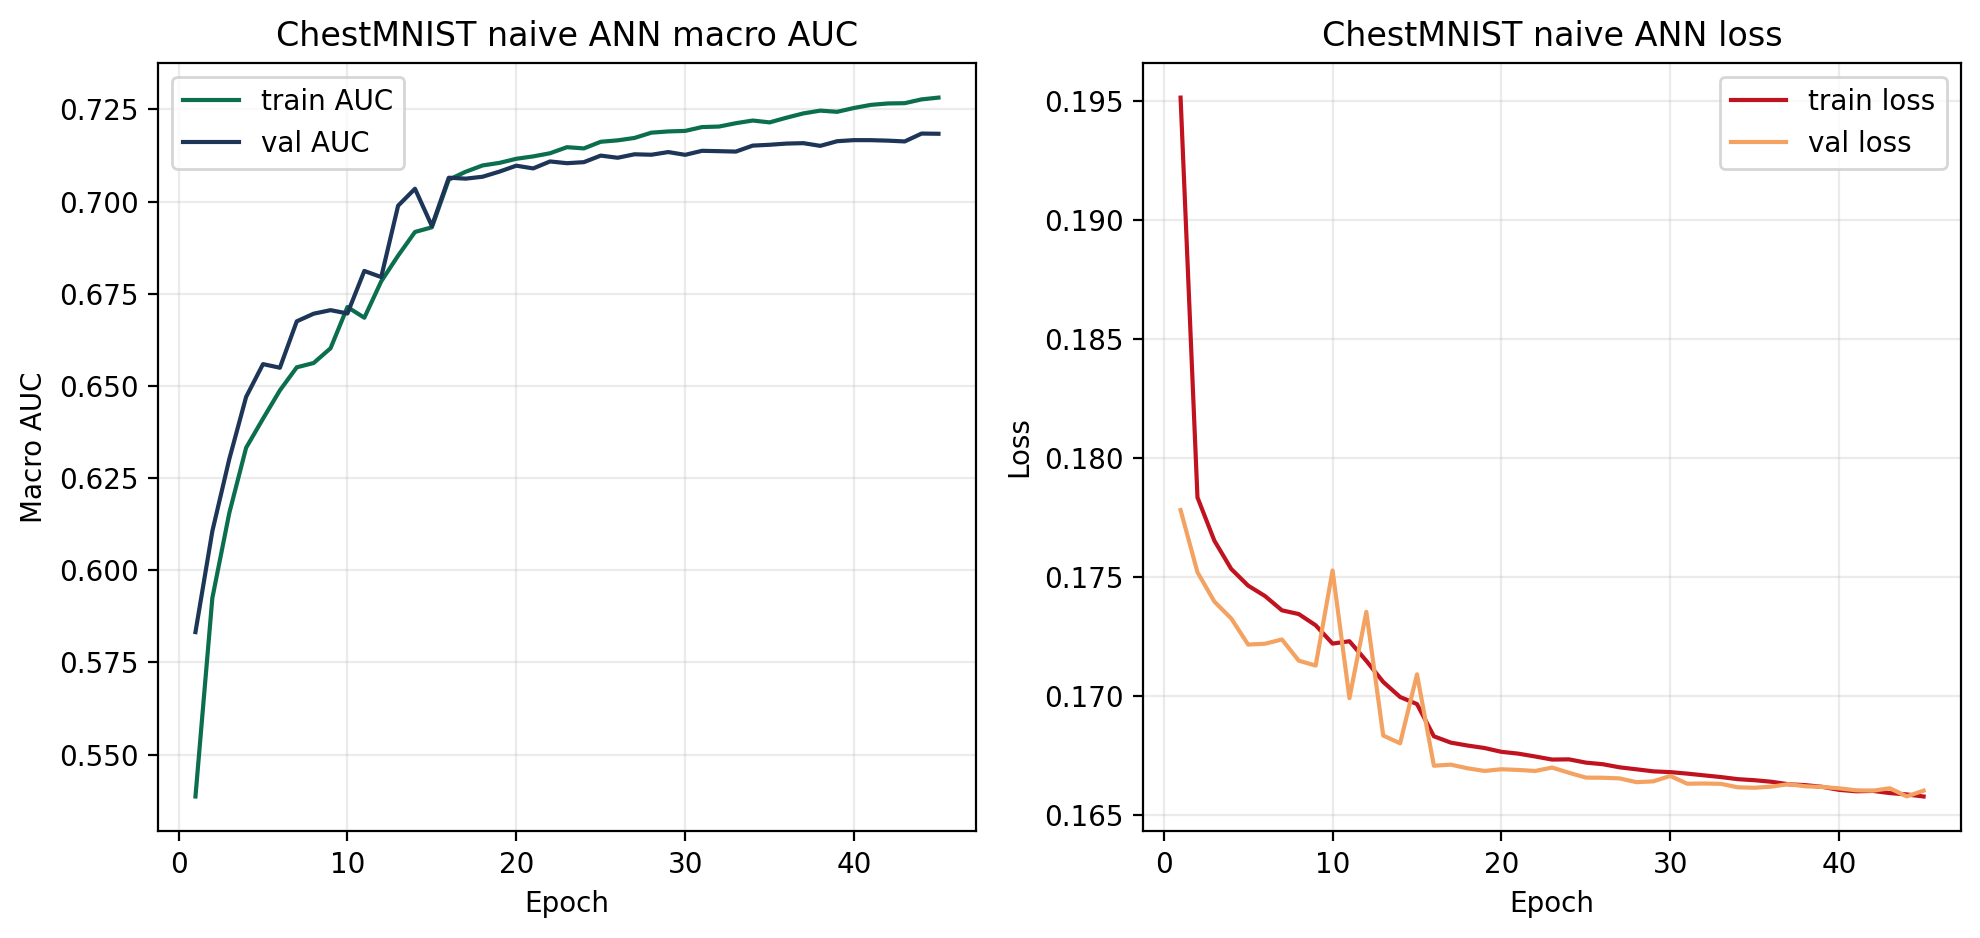
\includegraphics[width=0.95\textwidth]{figures/chestmnist-ann/training_curves.png}
  \caption{Diễn biến macro AUC và loss của baseline naive ANN trên ChestMNIST trong 45 epoch.}
  \label{fig:chestmnist-training-curves}
\end{figure}

\begin{figure}[H]
  \centering
  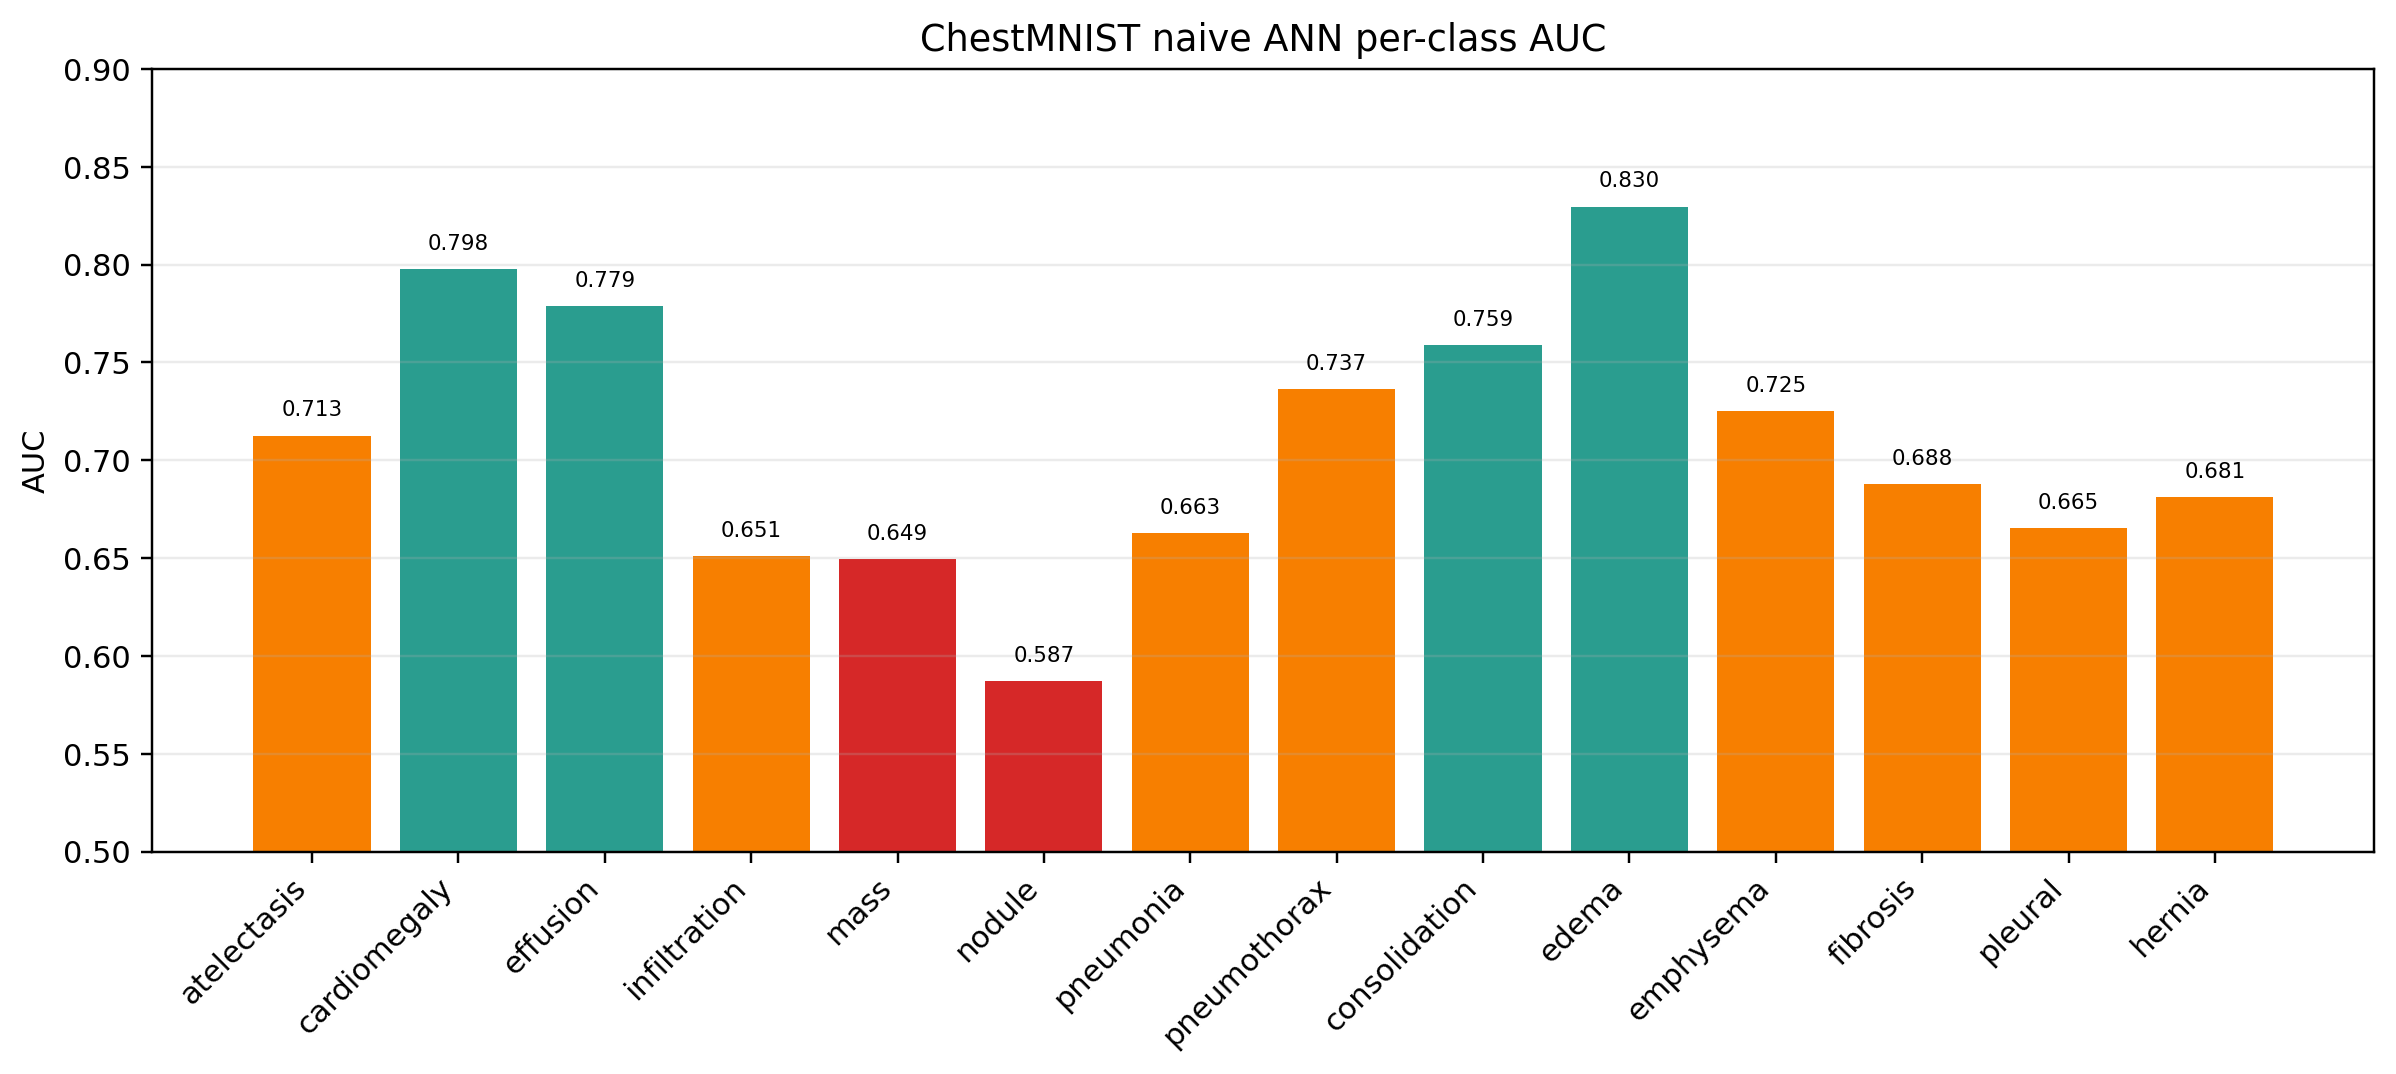
\includegraphics[width=0.95\textwidth]{figures/chestmnist-ann/per_class_auc.png}
  \caption{AUC theo từng nhãn bệnh của baseline naive trên ChestMNIST.}
  \label{fig:chestmnist-per-class-auc}
\end{figure}

\begin{figure}[H]
  \centering
  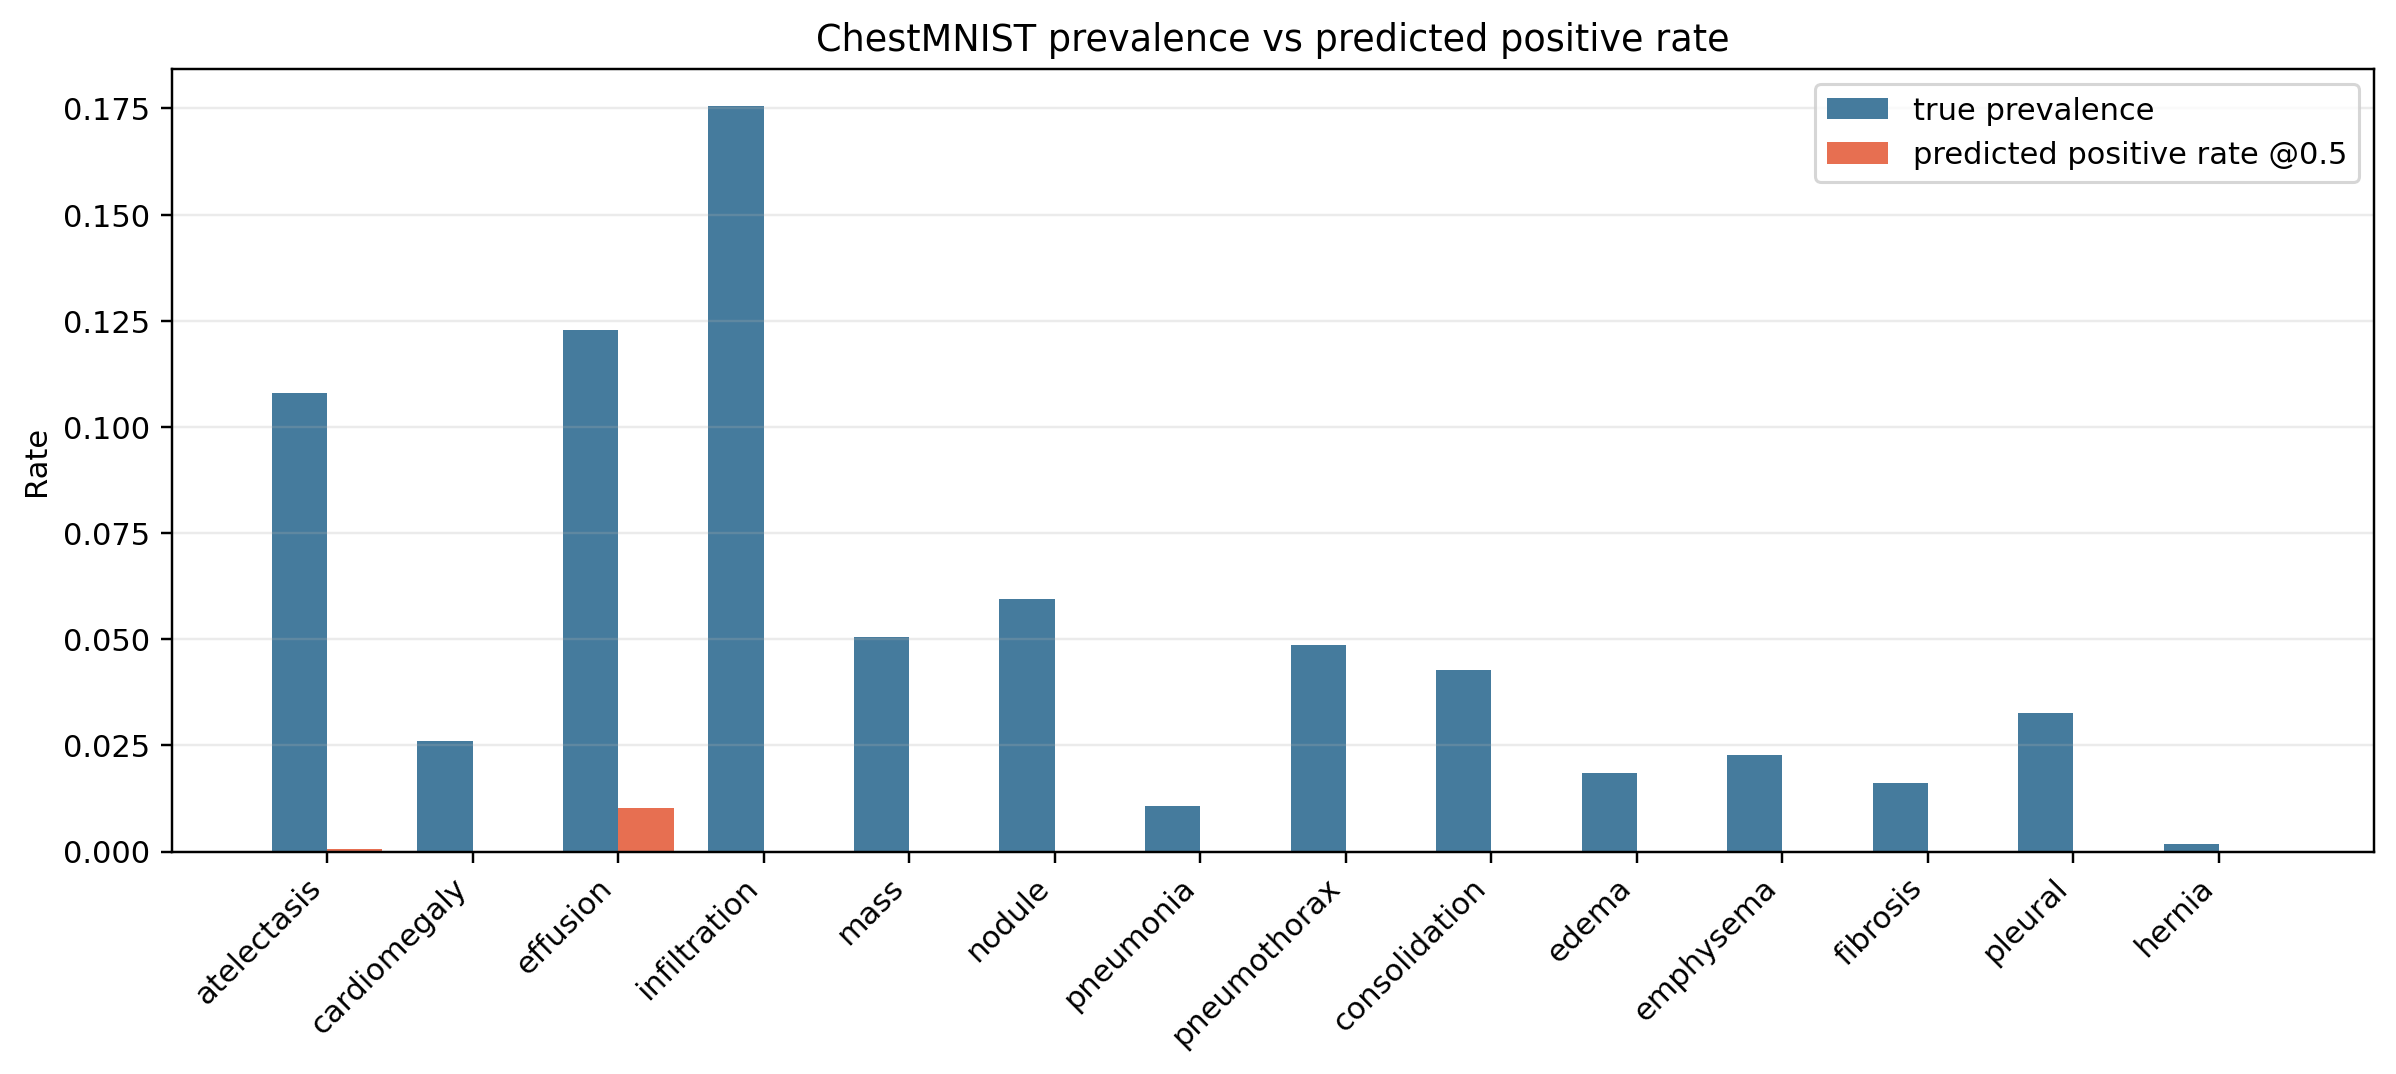
\includegraphics[width=0.95\textwidth]{figures/chestmnist-ann/prevalence_vs_pred_rate.png}
  \caption{So sánh tỷ lệ dương thật và tỷ lệ dương dự đoán ở ngưỡng $0.5$ của baseline naive trên ChestMNIST.}
  \label{fig:chestmnist-prevalence-vs-pred-rate}
\end{figure}

\begin{table}[H]
\centering
\caption{Một số nhãn dễ và khó nhất của baseline naive trên ChestMNIST}
\label{tab:chestmnist-per-class-auc}
\begin{tabular}{l c c c c}
\toprule
Nhãn & AUC & F1 & Tỷ lệ dương thật & Tỷ lệ dương dự đoán \\
\midrule
Edema & 0.8296 & 0.0000 & 0.0184 & 0.0000 \\
Cardiomegaly & 0.7978 & 0.0000 & 0.0259 & 0.0000 \\
Effusion & 0.7787 & 0.0891 & 0.1228 & 0.0103 \\
Nodule & 0.5872 & 0.0000 & 0.0595 & 0.0000 \\
Mass & 0.6494 & 0.0000 & 0.0505 & 0.0000 \\
Infiltration & 0.6508 & 0.0020 & 0.1755 & 0.0002 \\
\bottomrule
\end{tabular}
\end{table}


Baseline naive đạt \textit{test macro AUC} $0.7088$ và \textit{test ACC} $0.9475$. AUC cho thấy mô hình mới chỉ học được tín hiệu phân biệt ở mức vừa phải, trong khi ACC rất cao chủ yếu vì dữ liệu có quá nhiều nhãn âm. Hình prevalence-vs-pred-rate cho thấy mô hình gần như đoán âm cho phần lớn nhãn ở ngưỡng $0.5$, nên ACC cao nhưng chưa phản ánh tốt khả năng phát hiện ca bệnh thật.

Từ kết quả này, có thể thấy vấn đề chính không phải ANN hoàn toàn bất lực trước ảnh X-quang, mà là động lực học huấn luyện hiện tại quá thiên về việc giữ nhãn âm. Vì vậy, bước cải tiến kế tiếp hợp lý nhất là thêm weighted loss và cross-validation để buộc mô hình chú ý nhiều hơn tới ca dương và ổn định hơn qua nhiều fold.

\subsection{Weighted ANN với cross-validation nội bộ}

Kết quả của baseline naive cho thấy hai vấn đề xuất hiện đồng thời. Thứ nhất, raw pixel thuần vẫn chứa tín hiệu phân biệt nhất định, thể hiện qua macro AUC vượt rõ mức ngẫu nhiên; tuy nhiên tín hiệu đó chưa đủ mạnh để đưa mô hình lên gần các benchmark tốt hơn. Thứ hai, mô hình có xu hướng chọn nghiệm an toàn theo hướng giữ nhiều nhãn âm, nên ACC cao nhưng chất lượng tách ca bệnh theo AUC còn hạn chế. Từ insight này, bước cải tiến hợp lý không phải là thêm handcrafted feature ngay lập tức, mà trước hết phải sửa đúng động lực học huấn luyện để mô hình coi trọng nhãn dương hơn và đánh giá nội bộ ổn định hơn trên tập train.

Biến thể thứ hai vì vậy vẫn giữ đầu vào raw pixel để cô lập ảnh hưởng của kỹ thuật huấn luyện, nhưng thay đổi đồng thời cả kiến trúc và protocol. MLP được mở rộng thành:
\[
784 \rightarrow 1024 \rightarrow 512 \rightarrow 256 \rightarrow 14.
\]
Chiều rộng tầng đầu tăng lên $1024$ để ANN có đủ năng lực biểu diễn hơn cho ảnh X-quang, vốn có cấu trúc khó hơn đáng kể so với chữ số viết tay và có nhiều tổn thương chỉ biểu hiện bằng thay đổi texture rất nhẹ. Hai tầng sau giảm dần về $512$ và $256$ để nén dần biểu diễn đã học, tránh giữ kích thước ẩn lớn suốt toàn mạng khiến số tham số tăng nhanh nhưng không bổ sung tương xứng về khả năng tổng quát hóa. BatchNorm được thêm để ổn định phân phối kích hoạt giữa các tầng ẩn, còn Dropout giúp giảm sự phụ thuộc quá mức giữa các neuron trong bối cảnh số nhãn dương tương đối ít. Nói cách khác, phương pháp này không chỉ rộng hơn baseline, mà còn được tổ chức theo hướng “mở rộng để hấp thụ tín hiệu yếu, rồi nén dần để giữ đặc trưng cần thiết”.

Loss được đổi thành BCEWithLogitsLoss có \textit{pos\_weight}. Lý do là ChestMNIST bị mất cân bằng lớp mạnh: với nhiều nhãn bệnh, số mẫu âm áp đảo số mẫu dương. Nếu mọi nhãn đều bị phạt ngang nhau, quá trình tối ưu dễ nghiêng về chiến lược bảo thủ là ưu tiên đoán âm để giảm loss tổng thể. \textit{pos\_weight} làm tăng chi phí của việc bỏ sót nhãn dương, nên gradient thu được từ các ca bệnh trở nên đủ lớn để cạnh tranh với khối lượng mẫu âm. Nói cách khác, kỹ thuật này không nhằm tăng ACC, mà nhằm ép mô hình học tín hiệu bệnh thay vì chỉ dựa vào phân bố lớp.

Cross-validation nội bộ được thêm vì hai lý do. Thứ nhất, nếu chỉ chia train một lần, kết quả sẽ phụ thuộc khá mạnh vào cách chia trong bối cảnh dữ liệu đa nhãn và mất cân bằng. \textit{3-fold multilabel stratified cross-validation} giữ phân bố nhãn ổn định hơn giữa các fold, từ đó cho phép quan sát chất lượng huấn luyện nội bộ đáng tin cậy hơn. Thứ hai, ba mô hình thu được từ ba fold có thể ensemble ở bước test. Với ANN trên dữ liệu khó như ChestMNIST, ensemble các fold thường giúp giảm phương sai giữa các nghiệm tối ưu cục bộ và cải thiện AUC ổn định hơn so với chỉ giữ một checkpoint đơn lẻ.

\begin{table}[H]
\centering
\caption{Kết quả của weighted cross-validation ANN ensemble trên ChestMNIST}
\label{tab:chestmnist-weighted-cv-results}
\begin{tabular}{l c}
\toprule
Chỉ số & Giá trị \\
\midrule
Số fold & 3 \\
Epoch mỗi fold & 25 \\
Kiến trúc mạng & $784 \rightarrow 1024 \rightarrow 512 \rightarrow 256 \rightarrow 14$ \\
Optimizer & AdamW \\
Learning rate & 0.001 \\
Weight decay & 0.0001 \\
Loss & BCEWithLogitsLoss(pos\_weight) \\
Ensemble test macro AUC & 0.7306 \\
Ensemble test ACC & 0.7141 \\
Ensemble test macro F1 & 0.1605 \\
\bottomrule
\end{tabular}
\end{table}

\begin{table}[H]
\centering
\caption{Một số nhãn tiêu biểu của weighted ANN ensemble trên ChestMNIST}
\label{tab:chestmnist-weighted-per-class}
\begin{tabular}{l c c c c c}
\toprule
Nhãn & AUC & F1 & Tỷ lệ dương thật & Tỷ lệ dương dự đoán & Threshold \\
\midrule
Edema & 0.8419 & 0.1136 & 0.0184 & 0.2248 & 0.50 \\
Cardiomegaly & 0.8247 & 0.1311 & 0.0259 & 0.2657 & 0.50 \\
Effusion & 0.7868 & 0.3739 & 0.1228 & 0.3902 & 0.50 \\
Nodule & 0.6049 & 0.1385 & 0.0595 & 0.4271 & 0.50 \\
Mass & 0.6691 & 0.1527 & 0.0505 & 0.3109 & 0.50 \\
Infiltration & 0.6554 & 0.3576 & 0.1755 & 0.3742 & 0.50 \\
\bottomrule
\end{tabular}
\end{table}


\begin{figure}[H]
  \centering
  
\includegraphics[width=0.95\textwidth]{figures/chestmnist-weighted-ann/model_comparison.png}
  \caption{So sánh test macro AUC và ACC giữa baseline naive và weighted CV ANN trên ChestMNIST.}
  \label{fig:chestmnist-model-comparison}
\end{figure}

\begin{figure}[H]
  \centering
  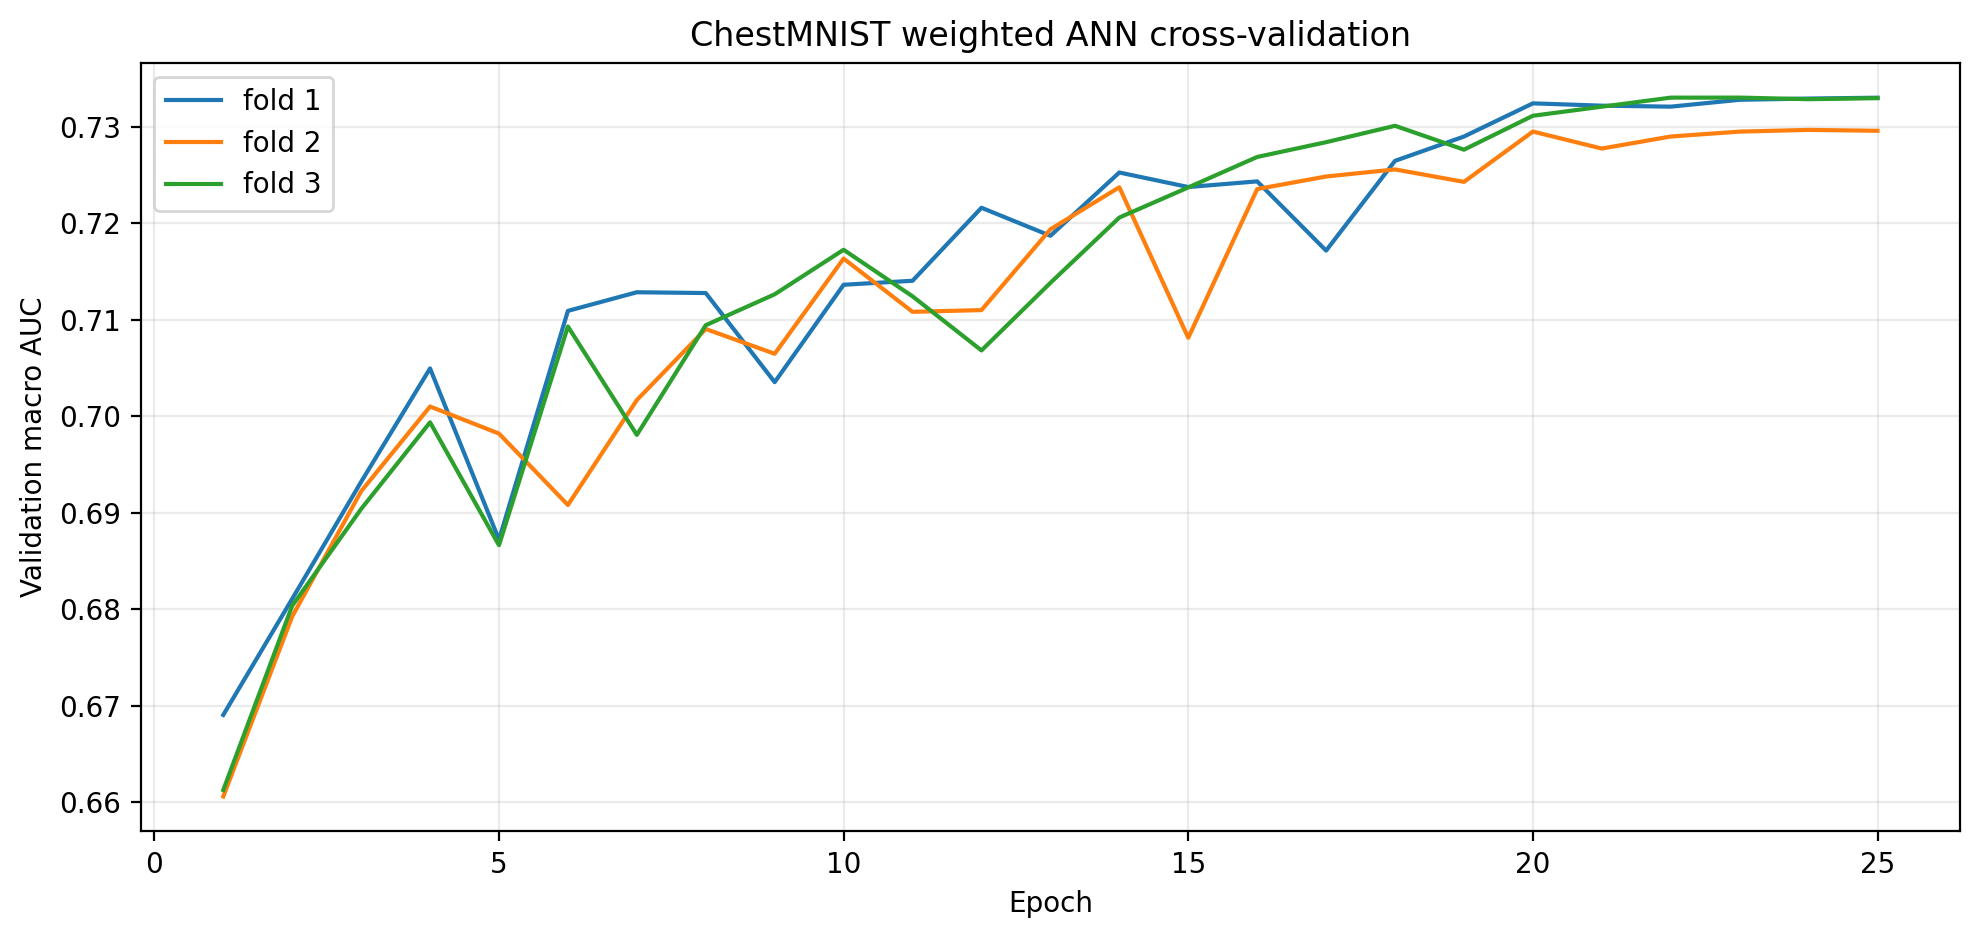
\includegraphics[width=0.95\textwidth]{figures/chestmnist-weighted-ann/cv_val_auc_curves.png}
  \caption{Đường cong validation macro AUC của 3 fold trong weighted CV ANN trên ChestMNIST.}
  \label{fig:chestmnist-cv-val-auc}
\end{figure}

\begin{figure}[H]
  \centering
  
\includegraphics[width=0.95\textwidth]{figures/chestmnist-weighted-ann/per_class_auc.png}
  \caption{AUC theo từng nhãn bệnh của weighted CV ANN ensemble trên ChestMNIST.}
  \label{fig:chestmnist-weighted-per-class-auc}
\end{figure}

\begin{figure}[H]
  \centering
  
\includegraphics[width=0.95\textwidth]{figures/chestmnist-weighted-ann/prevalence_vs_pred_rate.png}
  \caption{So sánh tỷ lệ dương thật và tỷ lệ dương dự đoán của weighted CV ANN ensemble trên ChestMNIST.}
  \label{fig:chestmnist-weighted-prevalence}
\end{figure}

Weighted CV ANN nâng \textit{test macro AUC} lên $0.7306$. Mặc dù \textit{test ACC} giảm xuống $0.7141$, đây lại là hướng cải thiện đúng với benchmark y sinh: mô hình bắt đầu chấp nhận dự đoán dương nhiều hơn, thay vì tối đa hóa số lượng nhãn âm đúng. Các đường cong validation AUC của ba fold cũng cho thấy chất lượng nội bộ giữa các lần chia không dao động quá lớn, tức là hướng cải tiến này không chỉ tăng trên một split cụ thể mà có độ ổn định tốt hơn baseline.

Sau bước này, insight rút ra là: thay đổi động lực học huấn luyện đã giúp ANN khai thác raw pixel tốt hơn, nhưng bản thân raw pixel vẫn chưa đủ giàu thông tin để đưa AUC lên sát các mốc benchmark mạnh hơn. Do đó, bước tiếp theo hợp lý là giữ lại weighted loss cùng protocol cross-validation, rồi bổ sung các handcrafted feature phù hợp với ảnh X-quang để đưa tín hiệu texture và cấu trúc vào ANN mà không cần chuyển sang CNN.

\subsection{Feature-fusion lite ANN}

Sau phương pháp 2, vấn đề còn lại không còn nằm chủ yếu ở loss hay protocol, mà ở bản thân biểu diễn đầu vào. Raw pixel giữ được cường độ sáng tại từng vị trí nhưng không mã hóa tường minh các tính chất texture và cấu trúc vốn quan trọng trong ảnh X-quang. Đây là lý do phương pháp 3 chuyển sang hướng \textit{feature fusion}: thay vì buộc ANN tự suy ra toàn bộ texture từ pixel thô, ta chủ động đưa vào những descriptor cổ điển vốn đã phù hợp với dữ liệu mức xám y sinh.

Biến thể cuối cùng của chương này là \textit{feature-fusion lite ANN}. Mỗi ảnh được biểu diễn bởi bốn nhóm đặc trưng: raw pixel, HOG, LBP histogram và intensity histogram. Mỗi nhóm giữ một vai trò khác nhau: raw pixel bảo toàn cường độ gốc; HOG mã hóa hướng gradient và biên cấu trúc; LBP histogram nhấn mạnh texture cục bộ; intensity histogram mô tả phân bố mức xám toàn ảnh. Cách ghép này xuất phát trực tiếp từ giả thuyết rằng ảnh X-quang cỡ nhỏ cần đồng thời cả thông tin biên lẫn texture để ANN phân biệt tốt hơn giữa các mẫu có tổn thương và mẫu bình thường. Các đặc trưng được nối lại thành một vector chung, rồi đưa qua MLP:
\[
\text{feature fusion} \rightarrow 1024 \rightarrow 512 \rightarrow 256 \rightarrow 14.
\]
Kiến trúc ẩn được giữ cùng khung $1024 \rightarrow 512 \rightarrow 256$ như phương pháp 2 để phép so sánh tập trung vào tác động của đầu vào mới thay vì bị nhiễu bởi việc đổi mạng quá nhiều. Việc không thay phần thân mạng giúp kết luận cuối cùng rõ ràng hơn: nếu AUC tăng, nguồn cải thiện chủ yếu phải đến từ chất lượng biểu diễn đầu vào và cơ chế tối ưu, chứ không phải do mạng đột ngột sâu hơn hay rộng hơn. Loss được đổi tiếp thành weighted focal BCE. Nếu \textit{pos\_weight} ở phương pháp 2 giải quyết vấn đề mất cân bằng lớp ở mức toàn cục, thì focal term của phương pháp 3 đi thêm một bước nữa: giảm trọng số của các mẫu quá dễ và tập trung gradient nhiều hơn vào các ca khó hoặc còn bị nhầm. Điều này đặc biệt phù hợp khi đầu vào đã giàu tín hiệu hơn, vì mô hình cần ưu tiên học các ranh giới quyết định khó thay vì tiếp tục tối ưu những mẫu âm dễ.

Protocol huấn luyện vẫn là \textit{3-fold cross-validation} trên split train chính thức và ensemble các fold ở bước test. Việc giữ nguyên protocol này là có chủ đích: nhờ đó, mọi cải thiện AUC ở phương pháp 3 có thể được quy về feature engineering và focal-weighted optimization, thay vì đến từ thay đổi cách đánh giá.

\begin{table}[H]
\centering
\caption{Kết quả của feature-fusion lite ANN ensemble trên ChestMNIST}
\label{tab:chestmnist-lite-results}
\begin{tabular}{l c}
\toprule
Chỉ số & Giá trị \\
\midrule
Feature set & raw + HOG + LBP histogram + intensity histogram \\
Kiến trúc mạng & feature fusion $\rightarrow 1024 \rightarrow 512 \rightarrow 256 \rightarrow 14$ \\
Số fold & 3 \\
Epoch mỗi fold & 40 \\
Optimizer & AdamW \\
Learning rate & 0.001 \\
Weight decay & 0.0001 \\
Loss & Weighted focal BCEWithLogits \\
Ensemble test macro AUC & 0.7424 \\
Ensemble test ACC & 0.7301 \\
Ensemble test macro F1 & 0.1667 \\
\bottomrule
\end{tabular}
\end{table}


\begin{figure}[H]
  \centering
  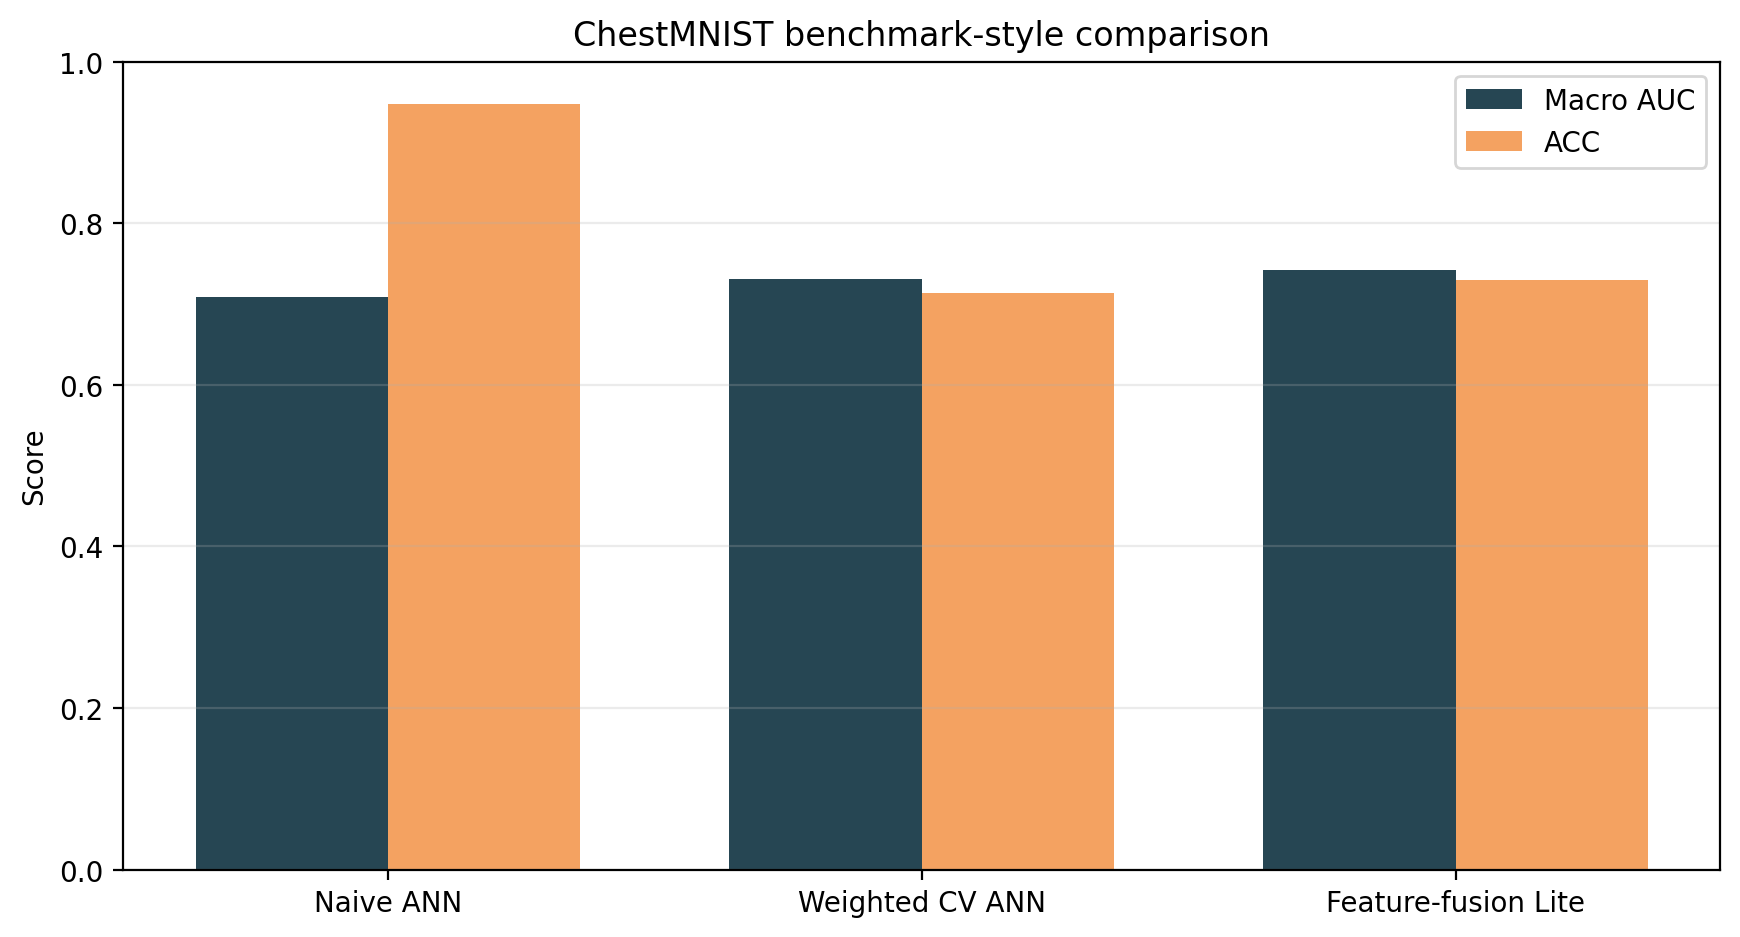
\includegraphics[width=0.95\textwidth]{figures/chestmnist-lite-ann/model_comparison.png}
  \caption{So sánh theo phong cách benchmark giữa ba cấu hình ANN trên ChestMNIST.}
  \label{fig:chestmnist-lite-model-comparison}
\end{figure}

\begin{figure}[H]
  \centering
  
\includegraphics[width=0.95\textwidth]{figures/chestmnist-lite-ann/per_class_auc.png}
  \caption{AUC theo từng nhãn bệnh của feature-fusion lite ANN trên ChestMNIST.}
  \label{fig:chestmnist-lite-per-class-auc}
\end{figure}

\begin{figure}[H]
  \centering
  
\includegraphics[width=0.95\textwidth]{figures/chestmnist-lite-ann/prevalence_vs_pred_rate.png}
  \caption{So sánh tỷ lệ dương thật và tỷ lệ dương dự đoán của feature-fusion lite ANN trên ChestMNIST.}
  \label{fig:chestmnist-lite-prevalence}
\end{figure}

Feature-fusion lite ANN đạt \textit{macro AUC} $0.7424$ và \textit{ACC} $0.7301$, trở thành cấu hình ANN tốt nhất hiện tại trên ChestMNIST trong repo. Mốc AUC này đã tiệm cận baseline AutoKeras trong benchmark chính thức của MedMNIST~\cite{medmnist_site}. Nói rõ hơn, AutoKeras là một công cụ AutoML xây trên Keras/TensorFlow, nên đây là một baseline mạnh và có uy tín, nhưng chưa phải mốc trần cao nhất của benchmark. Vì vậy, việc ANN thuần trong báo cáo đạt gần mức này có thể xem là kết quả tốt và đáng tin cậy, dù vẫn còn khoảng cách so với các baseline CNN như ResNet.

\section{Tổng hợp kết quả và nhận xét}

\begin{table}[H]
\centering
\caption{Kiến trúc ba biến thể ANN trên ChestMNIST}
\label{tab:chestmnist-ann-architecture-details}
\small
\begin{tabularx}{\textwidth}{>{\raggedright\arraybackslash}p{3.3cm} >{\raggedright\arraybackslash}p{3.1cm} >{\raggedright\arraybackslash}X >{\raggedright\arraybackslash}p{3.2cm}}
\toprule
Biến thể & Đầu vào & Kiến trúc & Thành phần chính \\
\midrule
Naive ANN & Raw $784$ & $784 \rightarrow 512 \rightarrow 256 \rightarrow 14$ & ReLU, BCEWithLogits \\
Weighted CV ANN & Raw $784$ & $784 \rightarrow 1024 \rightarrow 512 \rightarrow 256 \rightarrow 14$ & BN + Dropout + weighted BCE \\
Feature-fusion lite ANN & Raw + HOG + LBP + histogram & Feature fusion $\rightarrow 1024 \rightarrow 512 \rightarrow 256 \rightarrow 14$ & BN + Dropout + weighted focal BCE \\
\bottomrule
\end{tabularx}
\end{table}

\begin{table}[H]
\centering
\caption{Thông số huấn luyện của ba biến thể ANN trên ChestMNIST}
\label{tab:chestmnist-ann-hyperparameters}
\small
\begin{tabularx}{\textwidth}{>{\raggedright\arraybackslash}p{3.2cm} >{\raggedright\arraybackslash}p{3cm} >{\raggedright\arraybackslash}p{2.1cm} >{\raggedright\arraybackslash}X}
\toprule
Biến thể & Tối ưu hóa / loss & Batch/epoch & Thiết lập đặc trưng và đánh giá \\
\midrule
Naive ANN & Adam, BCEWithLogits & Theo notebook baseline / 45 & Raw pixel; dùng validation chính thức để theo dõi \\
Weighted CV ANN & AdamW, weighted BCE & 3 fold / 25 & Raw pixel; 3-fold multilabel stratified CV; ensemble fold \\
Feature-fusion lite ANN & AdamW, weighted focal BCE & 3 fold / 40 & Raw + HOG + LBP + histogram; 3-fold CV; ensemble fold \\
\bottomrule
\end{tabularx}
\end{table}

\begin{table}[H]
\centering
\caption{Logic chuyển từ một biến thể ANN sang biến thể kế tiếp trên ChestMNIST}
\label{tab:chestmnist-ann-iteration-logic}
\small
\begin{tabularx}{\textwidth}{>{\raggedright\arraybackslash}p{3.2cm} >{\raggedright\arraybackslash}X >{\raggedright\arraybackslash}X}
\toprule
Biến thể hiện tại & Điểm yếu quan sát được & Ý tưởng cho biến thể kế tiếp \\
\midrule
Naive ANN & AUC còn thấp; ACC cao nhưng chủ yếu do dự đoán âm nhiều & Thêm weighted loss và cross-validation để tăng khả năng tách ca bệnh \\
Weighted CV ANN & AUC tăng nhưng còn khoảng cách với benchmark mạnh hơn & Bổ sung handcrafted feature phù hợp với ảnh X-quang và dùng focal loss \\
\bottomrule
\end{tabularx}
\end{table}

\begin{table}[H]
\centering
\caption{So sánh hai cấu hình ANN trên ChestMNIST}
\label{tab:chestmnist-model-comparison}
\begin{tabular}{l c c c}
\toprule
Cấu hình & Test macro AUC & Test ACC & Ghi chú \\
\midrule
Naive ANN & 0.7088 & 0.9475 & BCE + $t=0.5$ \\
Weighted CV ANN & 0.7306 & 0.7141 & wBCE + CV + ensemble fold \\
Feature-fusion Lite ANN & 0.7424 & 0.7301 & feature fusion + focal + CV \\
\bottomrule
\end{tabular}
\end{table}


Các bảng tổng hợp cho thấy lộ trình cải tiến của Chương 3 khá nhất quán. Baseline naive cho ACC rất cao nhưng AUC còn thấp, vì mô hình hưởng lợi nhiều từ việc dự đoán âm. Weighted CV ANN sửa đúng điểm nghẽn này bằng cách thay đổi loss và protocol huấn luyện, từ đó nâng AUC lên rõ rệt. Feature-fusion lite ANN tiếp tục đẩy AUC lên $0.7424$ nhờ đưa thêm thông tin cấu trúc và texture phù hợp với ảnh X-quang vào đầu vào của ANN.

Kết luận cho Chương 3 có thể chốt bằng ba ý chính. Thứ nhất, baseline naive cho thấy raw pixel thuần vẫn học được tín hiệu phân biệt ở mức vừa phải theo AUC, nhưng chưa đủ để tạo ra một ANN mạnh trên dữ liệu y sinh đa nhãn. Thứ hai, bước cải tiến hiệu quả nhất không đến từ việc chỉ mở rộng MLP, mà từ việc thay đổi đúng động lực học huấn luyện bằng weighted loss, cross-validation và ensemble; chính tổ hợp này đã kéo macro AUC từ $0.7088$ lên $0.7306$. Thứ ba, cấu hình tốt nhất hiện tại là \textit{feature-fusion lite ANN} với macro AUC $0.7424$ và ACC $0.7301$, cho thấy việc đưa thêm HOG, LBP histogram và intensity histogram vào ANN là có giá trị thực nghiệm rõ ràng trên ChestMNIST. Vì vậy, insight quan trọng nhất của chương này là: với dữ liệu ảnh y sinh, hiệu quả của ANN phụ thuộc rất mạnh vào cách tổ chức đầu vào và cách thiết kế loss, chứ không thể chỉ kỳ vọng raw pixel phẳng tự mang đủ thông tin cho mô hình.

\chapter{Kết luận và nhận xét tổng thể}

\section{Bảng tổng hợp toàn bài}

\begin{table}[H]
\centering
\caption{Tổng hợp kết quả tốt nhất trên ba bộ dữ liệu}
\label{tab:overall-project-summary}
\begin{tabularx}{\textwidth}{l l l c >{\raggedright\arraybackslash}X}
\toprule
Bộ dữ liệu & ANN tốt nhất & Chỉ số chính & Kết quả & Insight chính \\
\midrule
MNIST & Single-branch ANN & Test accuracy & 99.14\% & Chuẩn hóa hình học và HOG giải quyết phần lớn khó khăn; augmentation cục bộ và two-branch không tạo thêm lợi ích rõ rệt. \\
FashionMNIST & Single-branch ensemble & Test accuracy & 91.68\% & HOG và tiền xử lý vẫn hữu ích, nhưng bước cải thiện tốt nhất là ensemble để giảm phương sai dự đoán giữa các mô hình đơn. \\
ChestMNIST & Feature-fusion lite ANN & Macro AUC / ACC & 0.7424 / 0.7301 & Weighted loss, cross-validation ensemble và feature fusion là ba thành phần quyết định để ANN cạnh tranh được trên dữ liệu y sinh đa nhãn. \\
\bottomrule
\end{tabularx}
\end{table}


\section{Đóng góp chính của bài}

Trong phạm vi yêu cầu của Lab 03, báo cáo này có bốn đóng góp chính. Thứ nhất, báo cáo đã thiết kế và triển khai đầy đủ các pipeline ANN cho ba nhóm dữ liệu khác nhau: MNIST Handwritten, FashionMNIST và ChestMNIST. Thứ hai, mỗi bài toán đều không dừng ở một mô hình duy nhất mà được phát triển theo chuỗi baseline $\rightarrow$ cải tiến $\rightarrow$ đánh giá lại, nhờ đó có thể chỉ ra khá rõ thành phần nào thực sự tạo ra cải thiện. Thứ ba, báo cáo đã phân tích kết quả ở cả mức chỉ số tổng hợp lẫn mức lỗi điển hình, từ đó sinh ra các biến thể kế tiếp trên cơ sở thực nghiệm thay vì thử ngẫu nhiên. Thứ tư, báo cáo đã rút ra được các hướng cải tiến cụ thể cho từng bộ dữ liệu, thay vì chỉ kết luận chung rằng ``mô hình tốt hơn''.

\section{Kết luận thực nghiệm}

Ba nhóm thí nghiệm trên MNIST, FashionMNIST và ChestMNIST cho thấy cùng một xu hướng khá nhất quán: ANN thuần vẫn có thể đạt kết quả tốt nếu đầu vào được tổ chức hợp lý, nhưng hiệu quả của ANN phụ thuộc rất mạnh vào tiền xử lý, đặc trưng hóa và chiến lược tối ưu. Ở cả ba bộ dữ liệu, baseline đơn giản nhất luôn đóng vai trò mốc so sánh cần thiết để trả lời đúng câu hỏi đầu tiên của đề bài: ANN thuần trên raw pixel đi được tới đâu trước khi thêm các kỹ thuật khác.

Với \textbf{MNIST}, kết luận thực nghiệm rõ nhất là: cấu hình \textit{single-branch ANN} là lựa chọn tốt nhất với test accuracy $99.14\%$. Bước cải thiện quyết định nằm ở \textit{deslant + recenter + HOG}; trong khi đó, augmentation cục bộ và two-branch không tạo thêm lợi ích đáng kể. Vì vậy, với một bộ dữ liệu sạch như MNIST, ANN thuần hoàn toàn đủ mạnh nếu được cung cấp đúng biểu diễn đầu vào.

Với \textbf{FashionMNIST}, kết luận quan trọng nhất là: khó khăn chính không còn nằm ở việc thiếu đặc trưng toàn cục, mà nằm ở độ chồng lấn hình dáng giữa các lớp áo. Trong bối cảnh đó, cấu hình tốt nhất lại là \textit{ensemble của ba mô hình single-branch ANN} với $91.68\%$, chứ không phải two-branch hay region-focused feature fusion. Nói cách khác, trên FashionMNIST, bước cải thiện hiệu quả nhất là giảm phương sai dự đoán bằng ensemble.

Với \textbf{ChestMNIST}, cách chấm phải bám theo benchmark chuẩn là AUC và ACC. Kết quả tốt nhất hiện tại là \textit{feature-fusion lite ANN} với macro AUC $0.7424$ và ACC $0.7301$. Điều này cho thấy trên dữ liệu y sinh đa nhãn, ANN chỉ trở nên cạnh tranh khi đi cùng weighted loss, cross-validation ensemble và feature engineering phù hợp với texture cũng như cấu trúc mức xám của ảnh X-quang.

Nhìn ở mức tổng quát, bài học lớn nhất của toàn bộ báo cáo là: ANN không hề vô dụng trên dữ liệu ảnh, nhưng muốn ANN hiệu quả thì không thể chỉ tăng độ sâu hoặc độ rộng của MLP một cách cơ học. Điều quyết định hơn nằm ở việc tổ chức đầu vào đúng, chọn loss đúng và đánh giá đúng theo bản chất của từng bộ dữ liệu.

\section{Hạn chế cốt lõi}

Tuy vậy, báo cáo hiện tại vẫn có một giới hạn quan trọng. Tất cả các mô hình trong Lab 03 đều thuộc họ ANN thuần theo kiểu \textit{fully-connected}, nên chúng xem ảnh chủ yếu như một vector đặc trưng đã được trải phẳng. Cách làm này giúp việc phân tích và thiết kế feature engineering trở nên rõ ràng, nhưng đồng thời bỏ qua một giả định rất quan trọng của dữ liệu ảnh: các pixel gần nhau trong không gian thường có quan hệ chặt chẽ với nhau, còn các mẫu hình cục bộ như cạnh, góc, texture hay cấu trúc biên thường lặp lại ở nhiều vị trí khác nhau.

Đây chính là lý do sâu xa khiến ANN thuần trong báo cáo phải dựa nhiều hơn vào tiền xử lý, handcrafted feature và ensemble để bù lại những gì bản thân kiến trúc chưa nắm bắt được. Cũng vì giới hạn này mà khoảng cách với các benchmark mạnh hơn vẫn còn tồn tại. Trên FashionMNIST, benchmark công khai vẫn có những phương pháp vượt mốc hiện tại của báo cáo~\cite{fashionmnist_repo}. Trên ChestMNIST, dù cấu hình tốt nhất của báo cáo đã tiệm cận baseline AutoKeras, kết quả vẫn còn cách một khoảng đáng kể so với các baseline CNN mạnh hơn trong benchmark chính thức của MedMNIST~\cite{medmnist_site}.

\section{Đề xuất cải tiến theo từng bộ dữ liệu}

Với \textbf{MNIST}, hướng cải tiến hợp lý nhất không phải là thêm nhiều kỹ thuật mới, mà là giữ cấu hình single-branch ANN như một mốc đủ tốt rồi dùng nó làm baseline sạch cho các bài toán khó hơn. Kết quả của chương này đã cho thấy rất rõ rằng khi dữ liệu đủ sạch và đã được chuẩn hóa hình học, augmentation cục bộ và two-branch không còn tạo thêm giá trị đáng kể. Vì vậy, nếu tiếp tục mở rộng trên MNIST thì hướng phù hợp hơn là kiểm tra tính tối giản của mô hình, chẳng hạn giảm số tầng hoặc giảm số chiều ẩn để tìm ra cấu hình gọn hơn nhưng vẫn giữ vùng $99\%$.

Với \textbf{FashionMNIST}, điểm nghẽn hiện tại nằm ở nhóm lớp có silhouette rất gần nhau như \textit{T-shirt/top}, \textit{Shirt}, \textit{Pullover} và \textit{Coat}. Vì ensemble đang là bước cải thiện hiệu quả nhất, hướng phát triển tự nhiên là giữ single-branch ensemble làm trục chính, rồi thử những đặc trưng cục bộ mạnh hơn đúng ở vùng thân trên, thay vì tiếp tục mở rộng MLP một cách thuần túy. Những hướng đáng kiểm chứng hơn là spatial pyramid HOG, contour-based descriptor hoặc patch-based MLP; mục tiêu của chúng là giữ được thông tin \textit{vị trí} của cổ áo, vai và tay áo, vốn là phần mà vector pixel phẳng hoặc HOG toàn ảnh còn mô tả chưa đủ tách bạch~\cite{fashionmnist_repo}.

Với \textbf{ChestMNIST}, kết quả hiện tại đã cho thấy ANN có thể đi khá xa nếu đầu vào và loss được thiết kế đúng, nhưng khoảng cách với benchmark CNN vẫn còn. Vì vậy, bước tiếp theo hợp lý nhất là mở rộng từ feature-fusion lite ANN sang các mô hình vẫn giữ tinh thần MLP nhưng biết khai thác cấu trúc không gian tốt hơn, chẳng hạn patch-based MLP hoặc các khối attention nhẹ trên vùng ảnh. So với MNIST và FashionMNIST, đây là bài toán mà hạn chế ``vector hóa ảnh'' của ANN thuần lộ ra rõ nhất, nên nếu muốn tiếp tục tăng AUC thì việc đưa quan hệ không gian cục bộ trở lại mô hình sẽ là hướng phát triển tự nhiên hơn là chỉ tăng thêm chiều rộng của tầng ẩn~\cite{medmnist_site}.

% !TeX root = ../main.tex


\chapter*{Tài liệu tham khảo}
\addcontentsline{toc}{chapter}{Tài liệu tham khảo}
\printbibliography[heading=none]

\end{document}
